\newcommand{\econtexRoot}{Paper/}
% The \commands below are required to allow sharing of the same base code via Github between TeXLive on a local machine and ShareLaTeX.  This is an ugly solution to the requirement that custom LaTeX packages be accessible, and that ShareLaTeX seems to ignore symbolic links (even if they are relative links to valid locations)
\providecommand{\econtex}{\econtexRoot/texmf-local/tex/latex/econtex}
\providecommand{\econtexSetup}{\econtexRoot/texmf-local/tex/latex/econtexSetup}
\providecommand{\econtexShortcuts}{\econtexRoot/texmf-local/tex/latex/econtexShortcuts}
\providecommand{\econtexBibMake}{\econtexRoot/texmf-local/tex/latex/econtexBibMake}
\providecommand{\econtexBibStyle}{\econtexRoot/texmf-local/bibtex/bst/econtex}
\providecommand{\notes}{\econtexRoot/texmf-local/tex/latex/handout}
\providecommand{\handoutSetup}{\econtexRoot/texmf-local/tex/latex/handoutSetup}
\providecommand{\handoutShortcuts}{\econtexRoot/texmf-local/tex/latex/handoutShortcuts}
\providecommand{\handoutBibMake}{\econtexRoot/texmf-local/tex/latex/handoutBibMake}
\providecommand{\handoutBibStyle}{\econtexRoot/texmf-local/bibtex/bst/handout}

  
\documentclass[titlepage]{\econtex}\newcommand{\texname}{ConsumptionHeterogeneity}
\usepackage{\econtexSetup}\usepackage{\econtexShortcuts}
%\usepackage[nolists,tablesfirst]{endfloat}
\usepackage{tikz}
\usepackage{caption}
\usepackage[standardsections]{scrhack}
\usepackage{titlesec}
\setcounter{secnumdepth}{4}
\usepackage{placeins}
\usepackage{pdfpages}
\usepackage{setspace}
\onehalfspacing
\doublespacing
\usepackage{booktabs,rotating}

%\DeclareDelayedFloatFlavor{sidewaystable}{table}
%\renewcommand{\theposttable}{\Roman{posttbl}}
%\renewcommand{\thepostfigure}{\Roman{postfig}}
\renewcommand{\thetable}{\Roman{table}}
\renewcommand{\thefigure}{\Roman{figure}}

\provideboolean{ifWeb}
\setboolean{ifWeb}{false}
\opt{Web}{\setboolean{ifWeb}{true}}

\ifthenelse{\boolean{ifWeb}}{\usepackage{grfext}
\PrependGraphicsExtensions*{.svg,.jpg,.JPG,.png,.PNG,.pdf,.PDF}
}{}


\titleformat{\paragraph}
{\sffamily\mdseries\normalsize}{\theparagraph}{1em}{}
\titlespacing*{\paragraph}
{0pt}{3.25ex plus 1ex minus .2ex}{1.5ex plus .2ex}

\hypersetup{pdfauthor={Edmund Crawley <edmund.s.crawley@frb.gov>, Andreas Kuchler <aku@nationalbanken.dk>},
            pdftitle={Consumption Heterogeneity: Micro Drivers and Macro Implications},
            pdfsubject={Consumption Heterogeneity: Micro Drivers and Macro Implications},
            pdfkeywords={Uncertainty, Consumption Dynamics, MPC; JEL: D12, D31, D91, E21},
            pdfproducer = {LaTeX with hyperref and thumbpdf},
            pdfcreator = {pdflatex}
            }

\newlength\TableWidth

\provideboolean{StandAlone}
\setboolean{StandAlone}{false}
\write18{\TabsDir/StandAloneOff.command} % Tell input files that they are being pulled in from the master (and are not standalone documents)

%rm%\provideboolean{PrintVersion}
%rm%\setboolean{PrintVersion}{false}
%rm%\setboolean{PrintVersion}{true}

%circled draws a circle around a number
\newcommand*\circled[1]{\tikz[baseline=(char.base)]{
		\node[shape=circle,draw,inner sep=2pt] (char) {#1};}}

\begin{document}\bibliographystyle{\econtexBibStyle}
\input Switches.tex
%
\includepdf[pages=-]{Frontpage.pdf}
\begin{verbatimwrite}{\jobname.title}
Consumption Heterogeneity: Micro Drivers and Macro Implications
\end{verbatimwrite}

%\hfill{\tiny \jobname}

\title{ 
	CONSUMPTION HETEROGENEITY: MICRO DRIVERS AND MACRO IMPLICATIONS}
	%Consumption Heterogeneity: \\ Micro Drivers and Macro Implications}

\ifthenelse{\boolean{ifWeb}}{
\author{
  Edmund Crawley\authNum 
   \and
 Andreas Kuchler\authNum  
}
}{
\author{
  Edmund Crawley\authNum   \\ {\small Federal Reserve Board}
  \and
  Andreas Kuchler\authNum    \\ {\small Danmarks Nationalbank}
}
} % End ifWeb

\keywords{Uncertainty, Consumption Dynamics, MPC}
\jelclass{D12, D31, D91, E21}
% \aspublished{Final version as published in [].}

\date{November 2019}
\maketitle

%\begin{center}
%Click \href{http://www.econ2.jhu.edu/jobmarket/2018/CrawleyES/JobPaper/JobPaperCrawleyES.pdf}{\textbf{here}} for latest version
%\end{center}

\begin{abstract}
%  \opt{JournalFormatting}{\doublespacing}
%  \begin{verbatimwrite}{./.abstract.metadata} 
	This paper explores the microfoundations of consumption models and quantifies the macro implications of consumption heterogeneity. We propose a new empirical method to estimate the response of consumption to permanent and transitory income shocks for different groups of households. We then apply this method to administrative data from Denmark. The large sample size, along with detailed household balance sheet information, allows us to finely divide the population along relevant dimensions. We find that households that stand to lose from an interest rate hike are significantly more responsive to income shocks than those that stand to gain. Following a 1-percentage-point interest rate increase, we estimate that consumption decreases by a 1/4 percentage point through this interest rate exposure channel alone, making this channel substantially larger than the intertemporal substitution channel that is at the core of representative agent New Keynesian models.
%  \end{verbatimwrite}{./.abstract.metadata} 
%  \input{./.abstract.metadata}
\end{abstract}


\begin{authorsinfo}
\name{Crawley: Federal Reserve Board, Constitution Avenue \& 20th Street NW, Washington, DC 20551, USA, \href{mailto:edmund.s.crawley@frb.gov}{\texttt{edmund.s.crawley@frb.gov}}.}
\name{Kuchler: Danmarks Nationalbank, Havnegade 5, 1093 Copenhagen K, Denmark, \href{mailto:aku@nationalbanken.dk}{\texttt{aku@nationalbanken.dk}}.}
\end{authorsinfo}
\thanks{Viewpoints and conclusions stated in this paper are the responsibility of the authors alone and do not necessarily reflect the viewpoints of Danmarks Nationalbank or the Federal Reserve Board. The authors wish to thank colleagues and participants at conferences and seminars at Banque de France, BLS, Bocconi University, Danish Ministry of Finance, Danmarks Nationalbank, Deutsche Bundesbank, European Central Bank, Federal Reserve Board, FDIC, Georgetown University, Johns Hopkins University, University of Bergamo, University of Copenhagen, and the Boston, San Francisco, and New York Feds for useful comments and suggestions.}

\titlepagefinish
\setcounter{page}{1}

\pagebreak
%rm%\provideboolean{SlidesInText}
%rm%\setboolean{SlidesInText}{true}
\section{Introduction}
How do differences in household consumption behavior affect the business cycle? Recent heterogeneous agent models suggest that wealth redistribution between households with high and low marginal propensity to consume (MPC) may play a dominant role in propagating macroeconomic shocks, particularly for monetary policy.\footnote{See, for example, \cite{kaplan_monetary_2016}; \cite{garriga_mortgages_2017}; and \cite{greenwald_mortgage_2018}.} Testing the microfoundations of these models empirically, and quantifying the macroeconomic importance of redistribution, often boils down to measuring how MPCs vary systematically over dimensions such as wealth and exposure to interest rate movements. However, shortcomings both in the empirical methods used to measure MPCs and in the available data have limited the literature's ability to do this reliably.

In this paper we overcome some of these shortcomings. We present a new method to measure MPCs from income and consumption panel data, building upon that of \cite{blundell_consumption_2008} (henceforth BPP). We then apply our method to different groups of households in administrative data from Denmark. We estimate the average MPC in the economy to be 0.5, close to estimates obtained from natural experiments. By contrast, using the BPP method on our data yields a much lower estimate of 0.12.

We follow BPP by imposing identifying restrictions on household income and consumption dynamics.\footnote{The BPP method, and those closely related to it, has become a standard tool in the consumption literature. See, for example, \cite{violante_wealthy_2014}; \cite{auclert_monetary_2017}; and \cite{manovskii_how_2017}} We make two improvements to the method. First, we explicitly model the time aggregated nature of income and consumption in our data. Time aggregation, overlooked in much of the household finance literature, can result in significant estimation bias if it is not explicitly modeled.\footnote{\cite{crawley_time_2019} shows that estimates of the elasticity of consumption to transitory income shocks using the BPP method depend strongly on the nature of time aggregation in the data. He shows the estimate of the elasticity of consumption to transitory income increases from to 0.05---the estimate in BPP---to 0.25 when the time aggregated nature of the PSID data is modeled.} Second, we allow complete freedom in how consumption responds to a transitory income shock for up to two years, after which we assume no further response. This short-term response contrasts with the assumption in BPP that consumption follows a random walk. The random walk assumption, incompatible with high MPCs, was previously thought to be benign for estimates of consumption responses to transitory shocks.\footnote{\cite{kaplan_how_2010} show that the estimate of the period one consumption response to transitory shocks in BPP is unaffected by assumptions on the path of consumption in following periods. This result does not hold for time aggregated data---in our data we would greatly overestimate MPCs if we assumed a random walk, see online appendix \ref{BPP_compare}.} However, this is not true for time aggregated data. A consequence of allowing freedom for two years is that our method requires a slightly longer panel than BPP, but we believe the robustness of our estimates to many forms of misspecification is worth this cost.

Our data consist of a panel of income and expenditure for the entire Danish population, along with details of the interest rate sensitivity of households' financial assets and liabilities that we require to estimate the redistribution effects of monetary policy. Income and wealth data are largely third-party reported to tax authorities and correspondingly accurate. Accordingly, we use the household budget constraint to back out expenditure from income and wealth.

Speaking to the microfoundations of consumption behavior, we uncover a clear negative monotonic relation between MPC and liquid wealth. We show that the sign of this relationship is in line with standard buffer-stock models, although the magnitude of MPCs, especially for households with the most liquid assets, is difficult to reconcile with theory. When we include illiquid wealth, such as housing, this monotonic relationship between wealth and MPC no longer holds: Those with close to zero net worth have higher MPCs than both those with negative and positive net worth. That liquid wealth is more predictive of MPCs than net worth is consistent with the wealthy hand-to-mouth model of \cite{violante_wealthy_2014}.

The strength of our method and data over previous studies can be seen when we quantify the size of monetary policy redistribution channels. We follow the decomposition of \cite{auclert_monetary_2017} who reports sufficient statistics that determine the effect of monetary policy redistribution on aggregate consumption. However, being limited by the econometric methods he has at hand as well as by publicly available data sources, he finds it challenging to get a clear picture of how MPCs vary over the dimensions he identifies as relevant, such as unhedged interest rate exposure.

Broadly speaking, in our data, we see three groups with distinct MPCs and exposure to interest rate movements: the ``poor hand-to-mouth,'' with MPCs around 0.8, who own few assets, liquid or otherwise and are not directly exposed to interest rates; the ``wealthy hand-to-mouth,'' with MPCs around 0.5, who typically own houses and have mortgages and other debts whose payments rise with interest rates; and the ``wealthy,'' a smaller group with MPCs around 0.25, who typically own houses and also have large liquid bank balances, and whose income rises with interest rates.\footnote{These groups loosely line up with those of the same name in \cite{violante_wealthy_2014}, who define wealthy hand-to-mouth as households with significant illiquid assets but little or no liquid assets. We observe that these three groups are naturally separated along the dimension of unhedged interest rate exposure. See figure \ref{fig:MPCAuclert} in section \ref{monetary_policy}.}

We estimate that a 1-percentage-point rise in the real interest rate, which redistributes wealth from the wealthy hand-to-mouth debtors who pay the higher rate to the wealthy creditors who receive it, reduces aggregate consumption by 26 basis points through this redistribution channel alone. This channel is absent in representative agent models in which the intertemporal substitution channel instead dominates.

We believe the rich detail we are able to provide on the relationships between MPC, home ownership, liquidity, and interest rate exposure could be used to discipline microfounded macroeconomic models going forward. Furthermore, a growing number of large, high-quality panel datasets on income and consumption are becoming available to economists, which increases the value of robust econometric methods that can uncover household behavior.\footnote{Panel data from financial aggregation platforms have been highly informative about consumption behavior, although access to these data by researchers is very restricted. See \cite{gelman_harnessing_2014}, \cite{ganong_consumer_2017}, and \cite{baker_debt_2015} for examples using U.S. data. \cite{vardardottir_liquid_2016} use data from Iceland.} Beyond the applications in this paper, our method has a wide variety of potential applications in the consumption, household finance, and labor literatures.

\section{Background}
The need for better methods and data to measure consumption behavior at the household level has grown with the increasing recognition that household heterogeneity may play a key role in macroeconomic dynamics. \cite{kaplan_microeconomic_2018} provide an overview of the theoretical literature incorporating household heterogeneity into models of economic fluctuations. Computational and methodological limitations, along with early work by \cite{krusell_income_1998} showing that the aggregate dynamics of a TFP shock were not much changed in a heterogeneous agent model, have resulted in a slow start for this literature. However, recent advances have allowed for a new generation of Heterogeneous Agent New Keynesian (HANK) models that, as their name suggests, combine elements from both the heterogeneous agent and New Keynesian literature. These models not only match the growing evidence on micro level consumption behavior, but also imply very different aggregate dynamics and/or propagation mechanisms following macroeconomic shocks, compared to their representative agent equivalents. In particular, the transmission mechanism of monetary policy can look very different in a HANK model.\footnote{For example, in the model of \cite{kaplan_monetary_2016}, the intertemporal substitution channel is dwarfed by indirect general equilibrium effects, in stark contrast to a representative agent model.}

While these HANK models make clear the potential importance of heterogeneity in economic fluctuations, particularly for monetary and fiscal policy, their quantitative results hinge on assumptions, such as the tenure of debt instruments and the government's fiscal rule, that were unimportant in representative agent models. Thus far the ability of these models to help us distinguish transmission channels \textit{empirically} has been limited. \cite{auclert_monetary_2017}, in contrast to the fully structural HANK models, takes a simplified approach to aggregate dynamics, and one that we will follow in this paper.\footnote{\cite{wong_population_2016} also takes an empirical approach by identifying how the consumption response to monetary policy shocks varies with age.} He derives a set of sufficient statistics, directly measurable from a suitable dataset, that is highly informative about the  relative size of different monetary policy transmission channels. His methodology benefits from being transparent and closely tied to the data, reducing the problem to that of measuring the distribution of MPCs across relevant dimensions of redistribution. However, as we will see in the following section, evidence on how MPCs vary across the population has been hard to come by.\footnote{\cite{fagereng_mpc_2016} also estimate Aulert's sufficient statistics, imputing MPCs from lottery winnings in Norway, but they are limited by sample size. \cite{ampudia_monetary_2018} look at differences in Auclert's statistics between European countries but do not attempt to estimate MPCs.} 

\subsection{Existing Empirical Evidence on Heterogeneity in Consumption Behavior} \label{MPCEmpirics}
Most micro empirical evidence on consumption behavior comes in the form of an estimate of the marginal propensity to consume out of a one time source of income over the following three months to one year. Table \ref{table:MPCLiterature} shows a selection of the population average estimates from the literature. Most of these studies do not have the power to say much if anything about heterogeneity within the population.

Three methods are used to empirically determine the marginal propensity to consume. The first is to identify a natural experiment and measure the consumption response to it, which is often done using the Consumer Expenditure Survey in the United States. For example, \cite{johnson_household_2006} use randomly assigned timing of 2001 tax rebates and questions in the Consumer Expenditure Survey to identify a three-month aggregate marginal propensity to consume of 0.2 to 0.4. Of the three methods, natural experiments likely have the strongest identification, but estimates vary, and there is no strong consensus. Identification issues arise as to when exactly households learn about the payment versus when it is received, and the extent to which external validity extends from these natural experiments to the kinds of transitory shocks found in heterogeneous agent models is unclear.\footnote{Many studies find a smaller MPC for positive shocks than negative shocks---for example, \cite{bunn_consumption_2018}. In this paper we implicitly assume that the response is symmetric. In reality, our estimates represent an average of positive and negative shock reactions.} As most of these studies rely on consumer survey data, they tend to lack power due to high measurement error and low sample sizes. As a result, they have produced very little evidence of how the MPC varies among different groups in the economy. A recent paper by \cite{fagereng_mpc_2016} overcomes some of these problems. By using lottery data, the shock to income is truly random.\footnote{We should note that even lottery winnings have some problems. First, the results hold for winners of the lottery who may not be representative of the wider population. Second the consumption response to a lottery win may be very different to other income shocks. For example, one may spend a significant portion of a small lottery win just celebrating the win.} They use registry data from Norway similar to the data we use from Denmark and have a sample of over 30,000 lottery winners over 10 years. As a result, they can identify the MPC for households with differing liquid wealth, as well as by the size of the lottery win. They find that households in the lowest quartile of liquid wealth have an MPC of approximately 0.61 over a six-month period, as opposed to 0.45 for households in the highest quartile of liquid wealth. In another study using data from a financial aggregator, \cite{gelman_what_2016} has enough power to identify large differences in the impulse response to a tax rebate at a monthly frequency between household quintiles of cash-on-hand.
\begin{sidewaystable} \small
	\caption{Estimates of the Marginal Propensity to Consume from Income Shocks}
	\label{table:MPCLiterature}
	\begin{minipage}{\textwidth}
		\input\econtexRoot/Tables/MPCLiterature.tex 
		\footnotesize{$^{\star}$ Elasticity. Methods: 1) Natural experiment 2) Survey question 3) Covariance restrictions \\
		This table is adapted from \cite{carroll_distribution_2017}.}
	\end{minipage}
\end{sidewaystable}

The second method is simply to ask individuals how much of a transitory income change they would consume, as was done in the Italian Survey of Household Income and Wealth in 2010 and the NY Fed's Survey of Consumer Expectations in 2016-17. \cite{jappelli_fiscal_2014} find an aggregate MPC of 0.48 using these Italian data and are able to identify clear differences across levels of liquid wealth. \cite{fuster_what_2018} find a lower aggregate MPC in the NY Fed's survey, but they find heterogeneity by both size and sign of the shock. While this method holds great promise, it is clearly limited by the accuracy of households' own response to the question.

The third method, which we will follow, is to impose covariance restrictions on panel data of income and consumption and use these to identify the consumption response to income shocks of differing persistence. This method has the advantage that it can be used in a panel dataset with no natural experiment, such as the Danish administrative data we use or the PSID. The most well-known paper to use this method is by \cite{blundell_consumption_2008}, who use imputed non-durable consumption data based on food expenditure reported in PSID data. They estimate a consumption elasticity (closely related to an MPC if households' consumption level is close to their income) and find very little consumption response to transitory shocks; however, as we will discuss in section \ref{TimeAgg}, this estimate is strongly downward biased.

This paper also adds to the limited literature on consumption responses to permanent shocks to income. Natural experiments for permanent shocks are very hard to come by. \cite{gelman_response_2016} use shocks to gasoline prices as a proxy for a permanent shock to income and find an MPC close to 1 across the population. BPP find a consumption elasticity to permanent shocks to income around 0.65 (the permanent shock elasticity is less affected by the time aggregation problem). For a more complete overview of the literature on consumption responses to income changes, see \cite{jappelli_consumption_2010}.

\section{Empirical Strategy} \label{empirical_strategy} 
We will take a reduced form approach to estimate four parameters: the variance of permanent and transitory income shocks and the marginal propensity to consume out of permanent and transitory income shocks. To do so, we will make identifying restrictions on income and consumption dynamics. Specifically, we will assume that income is made up of a permanent component that moves as a random walk and a transitory component with persistence of less than two years. For consumption, we assume it responds permanently to a permanent income shock but has a short-lived response of no more than two years to a transitory income shock. Our model will be in continuous time in order to correctly account for the time aggregated nature of our data. These restrictions allow us to calculate a set of observable moments with which we can estimate the four parameters of interest using GMM.

 While this strategy allows us to precisely estimate these quantities, in some ways it obscures from the key features of the data that are driving the results. Therefore, in the next section we build some intuition on where identification is coming from by running some simple regressions.

\subsection{Methodology Intuition}
In this section we present some very simple regressions of expenditure growth on income growth and compare them with what we would expect in some very well understood baseline models.

We will look at the estimate of $\beta^N$ in the model
\begin{align*}
    \Delta^N c_{it} = \alpha^N + \beta^N \Delta^N y_{it} + \varepsilon_{it}
\end{align*}
where $N$, the number of years over which growth is measured, varies from 1 to 10. Our full identification will come from the fact that transitory income shocks make up a relatively large proportion of the variance of income growth over a short period, while permanent income shocks dominate the variance of income growth over a long period.

Figure \ref{fig:GrowthReg} shows what we would expect to see under three well known models, as well as what we actually observe in the data. First, the blue horizontal line at zero shows what we would see in a complete markets model. With complete markets, all idiosyncratic shocks to income are insured against, resulting in no relation between idiosyncratic income and consumption growth. Second, the green horizontal line at 0.75 shows what we would see in a Solow model. Households in the Solow model do not optimize, but instead spend a constant proportion of their income each period---in this case, 0.75---regardless of transitory shocks. Third, the red, upward-sloping line shows the results for a typical buffer-stock saving model.\footnote{These regression results come the heterogeneous beta model in \cite{carroll_distribution_2017}, calibrated to match the distribution of liquid wealth in Denmark.} In this model the regression of consumption growth on income growth over one year yields a relatively small number as households are able to self-insure against the transitory shocks that dominate at this frequency. As the time period over which income growth is measured increases the observed income growth is proportionally more permanent and self-insurance is not possible. The red line asymptotes toward 1.0 as N gets large.
	\begin{figure} 
	\begin{centering}
		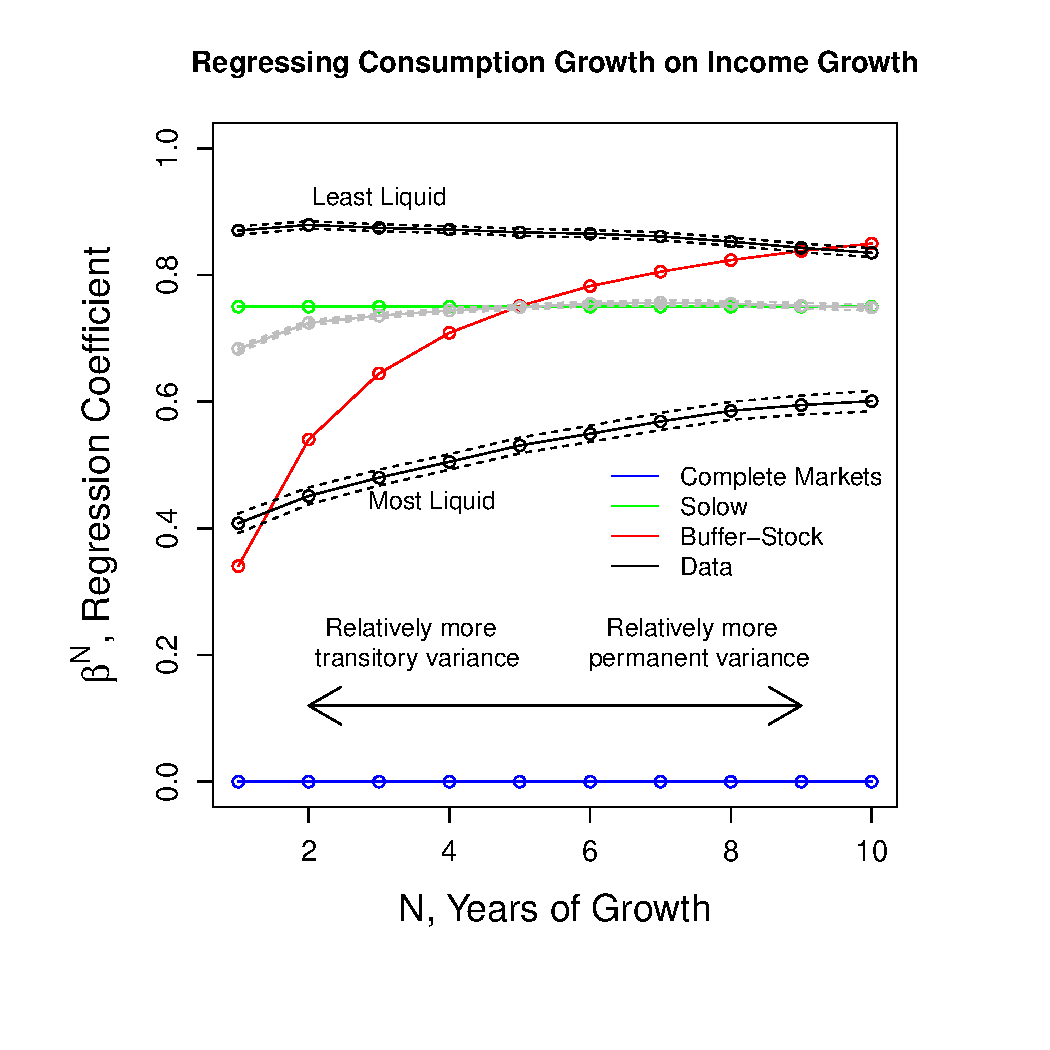
\includegraphics[scale=0.7]{\econtexRoot/Figures/basic_regression_liquid_wealth_level_lincome_head.pdf}
		\caption{Regression Coefficients of Consumption Growth on Income Growth}
		\label{fig:GrowthReg}
	\end{centering}
\end{figure}

The gray line, along with 95\% confidence intervals, shows the results of these regressions using all households in the Danish sample. It is striking that the data appear to be closest to the Solow model, with only a small decrease in the regression coefficient over short periods. However, aggregating all households in this way hides a large degree of heterogeneity, particularly across households with different levels of liquid wealth.

The two black lines show the regression coefficients where the sample is restricted to households in the lowest and highest quintiles of liquid wealth (averaged over the observed period), respectively. For households in the lowest quintile there is no evidence of consumption smoothing: the consumption response to income growth over one year is both high and almost identical to that over 10 years, strongly suggesting the MPCs for this group out of transitory and permanent shocks are similar and high. Indeed, this is what we find in section \ref{MPX_wealth}, and the result is highly robust to misspecification. Households in the top quintile of liquid wealth show a clear upward slope in figure \ref{fig:GrowthReg}, indicating a substantial degree of consumption smoothing. The fact that the regression coefficient for this group appears to asymptote well below 1 also suggests, in contrast to standard buffer-stock models, that the MPC out of permanent shocks for liquid households is significantly lower than 1.

\subsection{Identifying Restrictions} \label{cov_restrictions}
Next, we describe the restrictions we impose on income and consumption dynamics that allow us to identify the variance of permanent and transitory income shocks, as well as how households respond to them. 

\subsubsection{Income Dynamics}
Our identification of permanent and transitory income variance will follow the methodology of \cite{carroll_nature_1997} closely. As in their approach, we assume idiosyncratic income is composed of permanent and transitory components, where the permanent component follows a random walk and the transitory component persists for no more than two years. Our main innovation is to account for time aggregation by setting their discrete time model in continuous time and aggregating income over each year appropriately. We choose to model the level income process, rather than the log income process as in \cite{carroll_nature_1997}, as this allows more direct estimates of marginal propensities to consume.\footnote{In online appendix \ref{robustness} we get qualitatively similar results using a model of log income and expenditure.}

Our model is set in continuous time where each time period represents one year. We define two independent martingale processes (possibly with jumps), $P_t$ and $Q_t$, where $P_t$ will represent the \textit{flow} of permanent income at time $t$ and the change in $Q_t$ provides the transitory \textit{impulses} that generate the transitory income. We assume that for all  $s_1>s_2>s_3>s_4>0$:
\begin{align*}
\mathrm{Var}(P_{s_1}-P_{s_2})=(s_1-s_2)\sigma_P^2 \\
\mathrm{Cov}(P_{s_1}-P_{s_2},P_{s_3}-P_{s_4}) = 0 \\
P_s = 0 \qquad \text{if } s<0
\end{align*}
and similarly for $Q_t$. That is, these martingales have independent increments. As a useful benchmark, two Brownian motions satisfy these criteria.

The natural generalization of the MA(2) transitory income process from \cite{carroll_nature_1997} is to allow for a generically shaped transitory income shock that decays to zero in under two years.\footnote{Previous studies have found little evidence of transitory dynamics lasting more than one year, but to be conservative and in line with BPP we allow transitory income to persist for up to two years.} Figure \ref{fig:GenericTransitory} shows an example of such a transitory income shape $f(t)$, but the model also allows for completely transitory shocks in which case $f(t)$ would be a delta function with all the income from the transitory shocks arriving as a mass at the time of the shock. In this model the \textit{flow} of income arriving at time $t$ is given by the flow of permanent income and the sum of income arising from any transitory shocks to income that have occurred in the previous two years:
\begin{figure} 
	\begin{centering}
		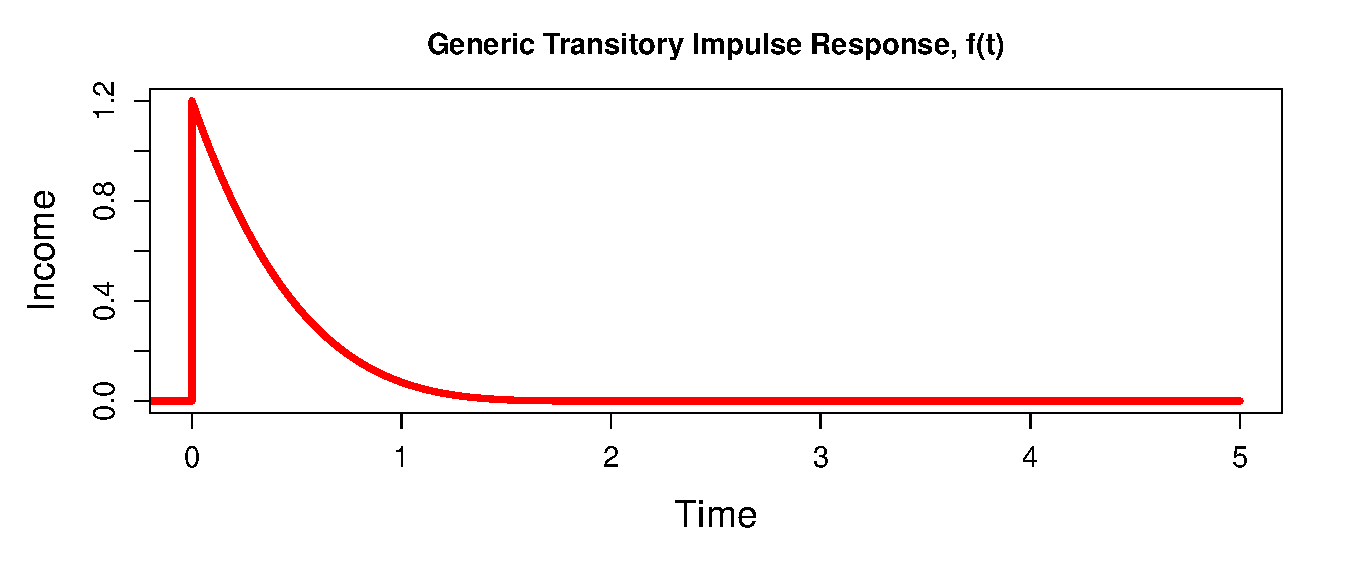
\includegraphics[scale=0.7]{\econtexRoot/Figures/GenericTransitory.pdf} 
		\caption{Generic Transitory Shock Impulse Response}
		\label{fig:GenericTransitory}
	\end{centering}
\end{figure}
\begin{align*}
y_t &= P_t + \int_{t-2}^{t} f(t-s)dQ_s
\end{align*}
We do not observe $y_t$ directly but instead $\bar{y}_T$, the time aggregated income over each one year period:
\begin{align}
\bar{y}_T = \int_{T-1}^{T} y_t dt \text{   for } T \in \{1,2,3...\}\label{income_TA}
\end{align}
Taking the $N^{th}$ difference for $N \geq 3$ we get:
\begingroup
\allowdisplaybreaks[0]
\begin{align}
\Delta^N \bar{y}_T &= \int_{T-1}^{T} y_t dt  - \int_{T-N-1}^{T-N} y_t dt  \nonumber \\ 
&= \int_{T-1}^{T} (T-s)dP_s  + (P_{T-1} - P_{T-N}) + \int_{T-N-1}^{T-N} (s-(T-2))dP_s \nonumber \\
& \qquad + \Big(\int_{T-1}^{T} \int_{t-2}^{t} f(t-s)dQ_t dt -\int_{T-N-1}^{T-N}\int_{t-2}^{t} f(t-s) dQ_t dt \Big) \label{deltaNy}
\end{align}
\endgroup
The variance of time aggregated income of an $N$ year period is therefore:\footnote{See online appendix \ref{sec:Identification} for full details of this derivation.}
\begin{align}
\mathrm{Var}(\Delta^N \bar{y}_T) &= (N-\frac{1}{3})\sigma^2_P +  2 \mathrm{Var}(\tilde{y}) \text{   for }n \geq 3 \label{variance}
\end{align}
This is similar to the discrete time model in \cite{carroll_nature_1997} except that the coefficient on permanent variance is $N-\frac{1}{3}$ in place of $N$. The transitory variance identified is the variance of ``total'' transitory income received in the year, $\tilde{y}$, where this is defined as\footnote{In the discrete time MA(2) model, $y_t = p_t + \varepsilon_t + \theta_1 \varepsilon_{t-1} + \theta_2 \varepsilon_{t-2}$, different definitions of transitory variance are used. \cite{carroll_nature_1997} estimate $(1+\theta_1^2 + \theta_2^2)\sigma_{\varepsilon}$ while \cite{blundell_consumption_2008} estimate $\sigma_{\varepsilon}$. Our definition of $\mathrm{Var}(\tilde{y})$ is the continuous time analog of \cite{carroll_nature_1997}. It is not clear what the analog of $\sigma_{\varepsilon}$ would be in continuous time.}
\begin{align}
\tilde{y_T} = \int_{T-1}^{T}\int_{t-2}^{t} f(t-s)dQ_s dt \label{tot_income}
\end{align}
Equation \ref{variance} shows that the variance of income growth grows linearly with the number of years of growth beyond three years. This result comes from the fact that the transitory component adds variance at the beginning and end of the growth period, but any transitory shock to income that occurs in the middle of the period does not affect income growth, as it will have decayed by the end of the measured period.

\subsubsection{Consumption Dynamics} \label{cons_dynamics}
Our approach will be to extend the identification of income variance by using growth over three, four and five years to also identify the covariance of income and consumption. In contrast to \cite{blundell_consumption_2008}, who assume that consumption follows a random walk, we will instead assume that the impulse response to a transitory shock follows a generic path, $g(t)$, that, like the transitory income shock, has fallen to zero two years after the news of the shock. Figure \ref{fig:GenericTransitoryBPP} shows possible paths for both income and consumption, along with the alternative random walk impulse response of BPP. The best evidence for the speed at which the consumption response decays comes from \cite{gelman_what_2016} and \cite{fagereng_mpc_2016}, both of which show that the response has entirely or almost entirely decayed two years after the shock. In section \ref{Consumption_persistence} we will show how this assumption may potentially bias the transitory consumption response down, but that this bias is small, especially for all but the most liquid households. We will maintain the assumption from BPP that the consumption response to a permanent shock to income follows a random walk proportional to the permanent shock. Under these assumptions the instantaneous flow of consumption is given by:	\begin{figure} 
	\begin{centering}
		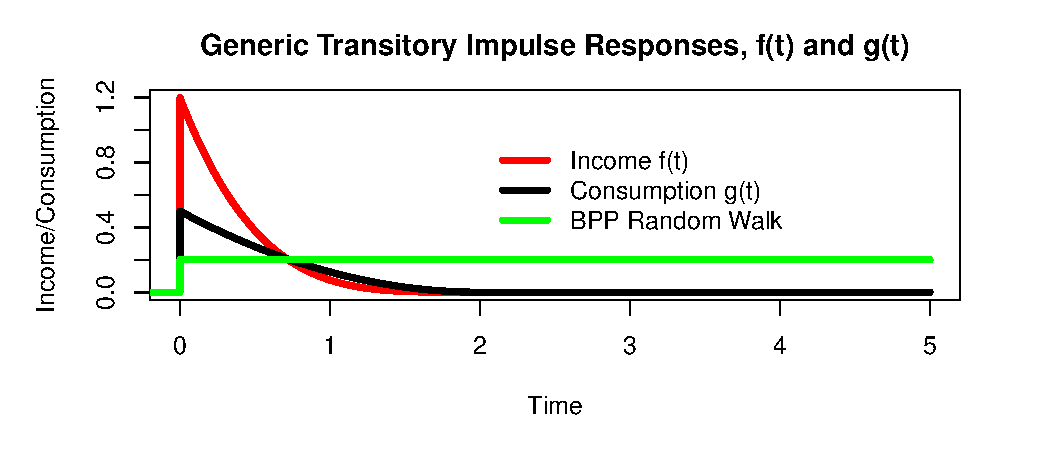
\includegraphics[scale=0.6]{\econtexRoot/Figures/GenericTransitoryConsumptionWithBPP.pdf} 
		\caption{Generic Transitory Shock Impulse Response}
		\label{fig:GenericTransitoryBPP}
	\end{centering}
\end{figure}
\begin{align*}
c_t  &= \phi P_s  + \int_{t-2}^{t} g(t-s)dQ_s  \\
\end{align*}
and the covariance of time aggregated income and consumption growth over $N \geq 3$ years is given by
\begin{align}
\mathrm{Cov}(\Delta^N \bar{c_T},\Delta^N \bar{y_T} ) &= \phi (N-\frac{1}{3}) \sigma^2_p + 2 \mathrm{Cov}(\tilde{c},\tilde{y}) \text{  for  } N\geq 3 \label{covariance}
\end{align}
where total transitory income, $\tilde{y}$, is given by equation \ref{tot_income} and total transitory consumption, $\tilde{c}$, is defined by
\begin{align}
\tilde{c_T} = \int_{T-1}^{T}\int_{t-2}^{t} g(t-s)dQ_s dt \label{tot_cons}
\end{align}

\subsection{Minimum Distance Estimation}
Using the equations for variance (\ref{variance}) and covariance (\ref{covariance}) of observed income and consumption growth over $N$ years for at least two different values of $N$, we are able to estimate the following four unknowns in which we are interested:\footnote{We have a total of 96 moments (we have eight consecutive five-year periods, each of which has three three-year growth periods, two four-year growth periods, and one five-year growth period. $8\times(3+2+1)=48$. Each of these growth periods has both a variance and a covariance moment, $48\times 2 = 96$). With only four parameters to estimate, the system is over identified. We strongly reject the null of the Sargen-Hansen J-test when run on our data, but this is not surprising given the sample size of our data.}
	\begin{itemize}
	\item[1.] $\sigma^2_p$ Variance of permanent shocks
	\item[2.] $\sigma^2_{\tilde{q}} = \mathrm{Var}(\tilde{y})$ Variance of transitory income received in a year
	\item[3.] $\phi$ Marginal Propensity to eXpend (MPX) w.r.t. permanent income
	\item[4.] $\psi = \frac{\mathrm{Cov}(\tilde{c},\tilde{y})}{\mathrm{Var}(\tilde{y})}$ Regression coefficient of transitory consumption w.r.t. transitory income over a year (MPX out of transitory income).
\end{itemize}
Our panel data cover 13 years and we choose to use growth over three, four and five years to balance greater identification (longer growth periods give more power) with three identification problems that grow with $N$. First, many households drop out of the sample if we demand they have reliable data for too many consecutive years. Second, if the permanent shock in fact decays slowly over time (e.g. is in fact AR(1)), the bias this introduces will be larger for large $N$. Third, the validity of running the regressions in levels (rather than logs) is reduced over large $N$ when the potential for the variance of income to change significantly from the start to the end of the sample is high. In section \ref{threats_to_identification} and online appendix \ref{robustness} we test the importance of these issues.

We follow \cite{blundell_consumption_2008} and use diagonally weighted minimum distance estimation, although our results are not significantly changed by using other popular weighting methods.\footnote{As our sample size is large, the motivation for using diagonally weighted minimum distance (DWMD) over optimal minimum distance (OMD) is small; see \cite{altonji_small-sample_1996}. We get very similar results using OMD. In general, our results may be subject to misspecification problems, but the sample size of our data means that standard errors are small.}

As the main part of our analysis will focus on the parameter $\psi$, it is worth describing exactly what this is and why we have labeled it the marginal propensity to expend out of transitory income. If we were able to exactly observe transitory income and consumption resulting from transitory income, then $\psi$ would be the regression coefficient of this transitory consumption on transitory income. If transitory income shocks have no persistence, this is approximately a six-month MPX (on average, the shock will happen six months into the year so that the regression will pick up the change in consumption in the following six months). If transitory income shocks have a little persistence (online appendix \ref{sample_selection} shows evidence of a small amount of transitory income persistence), $\psi$ can only loosely be interpreted as the MPX to an income shock, and the reader should bear in mind that the true interpretation is, ``if income is higher by one unit this year due to transitory factors, then consumption this year will be expected to be higher by $\psi$ units.''

\subsection{A Brief Introduction to the Time Aggregation Problem} \label{TimeAgg}
As previously explained, our identification comes from the shape of income and consumption covariance over increasing periods of time. An obvious question is why we have chosen not to use the well-known methodology of \cite{blundell_consumption_2008}, who achieve identification of transitory shocks from the fact that a transitory shock in period $t$ will mean-revert in period $t+1$.\footnote{\cite{kaplan_how_2010} show in discrete time simulations that the methodology works reasonably well for standard calibrations of buffer-stock models and end up concluding, ``The BPP insurance coefficients should become central in quantitative macroeconomics.'' However, some recent papers such as \cite{commault_how_2017} and \cite{hryshko_income_2018} have pointed to other potential problems of the methodology.} Unfortunately, the method is not robust to the time aggregation problem of \cite{working_note_1960}. While macroeconomists have long been aware of the importance of time aggregation in time series regressions (see \cite{campbell_consumption_1989} for a well-known example), the problem has been overlooked by the household finance and labor economics literature.\footnote{For examples, see \cite{moffitt_trends_2012}; \cite{meghir_income_2004}; \cite{nielsen_impact_2004}; \cite{heathcote_unequal_2010}; and more recent quantile regression approaches such as \cite{arellano_earnings_2017}.} We will therefore briefly describe the problem here. For a more detailed account with particular attention to BPP, see \cite{crawley_time_2019}.

Time aggregation occurs when a time series is observed at a lower frequency than the underlying data that generates it. For example, income is often observed at an annual frequency when it may in fact consist of paychecks arriving at a monthly, biweekly or irregular frequency. To transform income into an annual frequency, we sum up all the income that was received by a household during the year. The key insight of \cite{working_note_1960} is that even if there is no correlation between changes in income at the underlying frequency, changes in the resulting time aggregated series will show positive autocorrelation. The underlying intuition can be seen in figure \ref{fig:TimeAgg}, which shows the income process of a household that begins with an annual salary of \$50,000 and receives a permanent pay rise to \$100,000 mid-way through the second year. The solid line shows this jump in income flow occurring just once. The crosses show the income we actually observe in annual data. During the second year the household receives an annual \$50,000 salary for six months, followed by \$100,000 in the second six months, resulting in a reported income of \$75,000 for the entire year. The single shock to income therefore appears in the time aggregated data as two increases. In this way, an income change in one year is positively correlated with an income change in the following year, even if the underlying income process follows a random walk.\footnote{If all permanent shocks to income occurred on January 1 each year, then this would not hold. \cite{low_wage_2010} show that a significant portion of permanent income variance is explained by job mobility, which can occur at any point in the year.}
\begin{figure} 
	\begin{centering}
		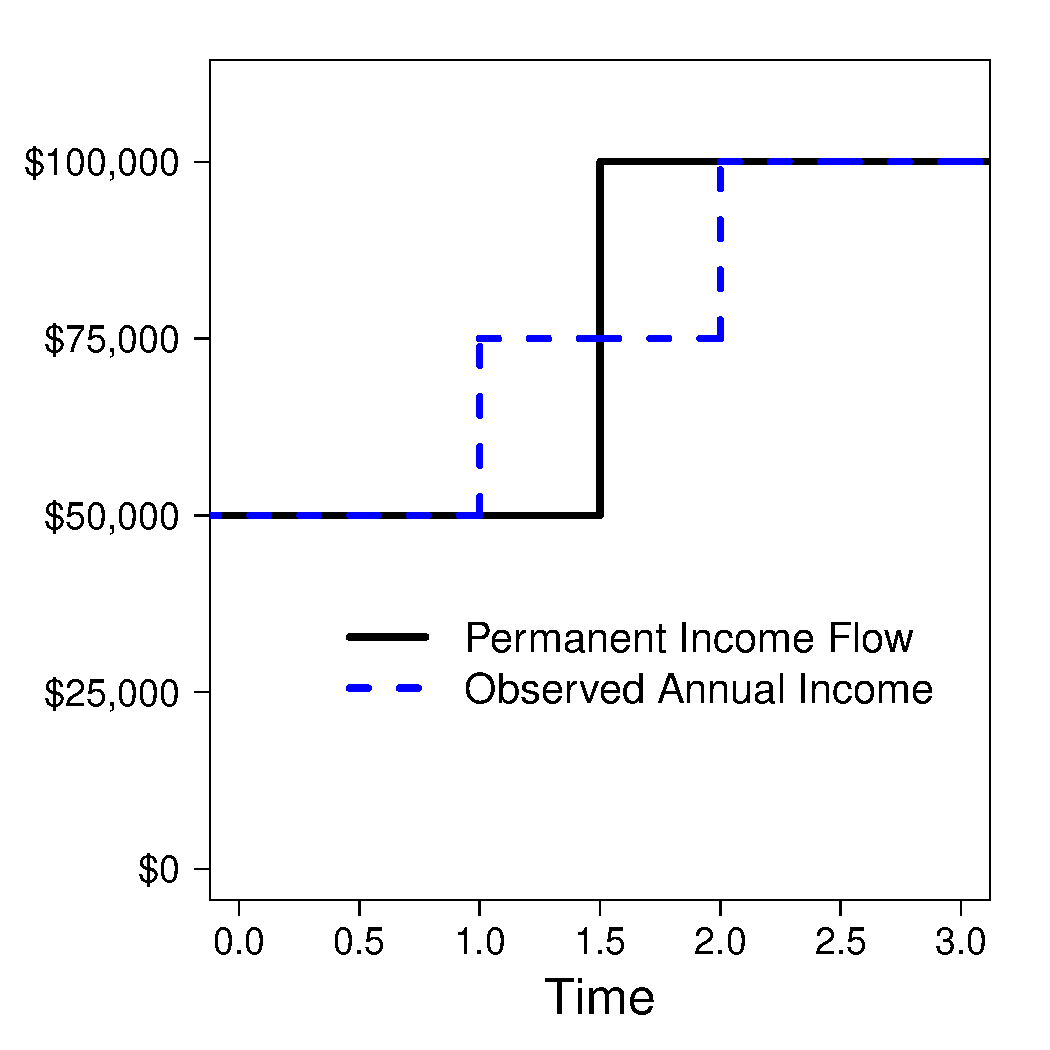
\includegraphics[scale=0.5]{\econtexRoot/Figures/TimeAgg_simple.pdf} 
		\caption{The Time Aggregation Problem}
		\label{fig:TimeAgg}
	\end{centering}
\end{figure}

While it would be possible to stick very closely to the original BPP model and adjust the covariance restrictions to take account of the time aggregation problem,\footnote{\cite{crawley_time_2019} takes this more straightforward approach using the same PSID data as used in BPP.} we have found that in practice the underlying assumptions made by BPP (in particular that consumption follows a random walk) do not fit with the data. The random walk assumption was previously thought to be benign. Not only were the estimates of the consumption response to transitory shocks in BPP small and consistent with such an assumption, \cite{kaplan_how_2010} show that without time aggregation, the BPP method correctly identifies the transitory consumption response in the period of the income shock regardless of the consumption dynamics going forward. This fact is again not robust to the time aggregation problem. With time aggregation taken into account, the estimates are highly sensitive to assumptions about short-term consumption dynamics.\footnote{See online appendix \ref{BPP_compare} to see how these different assumption change the estimates.} Therefore we have chosen to attain identification in a manner similar to \cite{carroll_nature_1997}, which allows us to be agnostic about the exact short-term dynamics of income and consumption.

\section{Data}
Our panel data on income and expenditure comes from Danish registry data from 2003-2015. These data have a number of advantages over survey-based measures. First, the sample contains millions of households rather than thousands. Second, households are required by law to report their data, so there is much less risk of selection bias through drop outs. Third, measurement error in income data is largely eradicated, as employees' income data is third party reported by their employer, compared to survey data where self-reported income has been shown to be particularly unreliable for irregular income.\footnote{See \cite{david_income_nodate} for a survey of income measurement error issues in survey data.}

\subsection{Income} \label{income}
We are interested in income and consumption decisions at the household level. We define a household as having either one or two adult members. Two adults are considered to be in the same household if they are living together and (i) are married to each other or have entered into a registered partnership, (ii) have at least one common child registered in the Civil Registration System or, (iii) are of opposite sex and have an age difference of 15 years or less, are not closely related and live in a household with no other adults.\footnote{Adults living at the same address but not meeting one of the three criteria are regarded as separate families. Children living with their parents are regarded as members of their parents' family if they are under 25 years old, have never been married or entered into a registered partnership, and do not themselves have children. A family meeting these criteria can consist of only two generations. If three or more generations live at the same address, the two younger generations are considered one family, while the members of the eldest generation constitute a separate family.} In the panel data, an individual's household will change if he or she gets married or divorced, which leads to some selection bias given that we require households to survive for at least five years. Following the literature, our baseline results will be reported using the labor income of the head of household.\footnote{See \cite{moffitt_income_2018} for an overview of the literature on income volatility in the PSID. In contrast to the PSID literature, we define the head of household as the highest earner over the 13-year period in our sample. We believe this definition better fits the social structure in Denmark.} We will use after tax and transfer income, as we are interested in the consumption response to these changes in income, although the method could be used to measure the extent of consumption insurance provided by the tax and transfer system. Our data come from the administrative records from the tax authority. The tax reporting system in Denmark is highly automated and individuals bear little of the reporting burden. For employees, income is reported by their employer and is thought to be highly accurate. The underground economy in Denmark is small. We remove business owners from the sample, as their income may be less accurately reported but, more importantly, the expenditure imputation method does not work well for them (see section \ref{cons_imputation}).



We work with the residual of income after controlling for observable characteristics of households that may affect their income and consumption. To start, we remove households in the top and bottom 1\% of the income distribution. We then normalize by average household income over the observed period and regress income on dummies for age, year, highest level of education, marital status, homeowner status, and number of children along with interaction of age with education, marital status, and homeowner status. We take the change in the residuals of this regression to be the unexpected income change for a household from one year to the next and remove households in the top and bottom 1\% of the unexpected income \textit{change} distribution.

\subsection{Imputed Expenditure} \label{cons_imputation}
Our expenditure data come from imputing expenditure from income and wealth. Along with other Scandinavian countries, Denmark is unusual in that tax reporting includes information about wealth along with income, a legacy from the wealth tax that was phased out between 1989 and 1997. Following the methodology from \cite{browning_imputing_2003} and \cite{fagereng_imputing_2015}, we impute expenditure using the identity
\begin{align*}
\bar{C_t} \equiv \bar{Y_t} - \bar{S_t} = \bar{Y_t} - P_t - \Delta NW_t 
\end{align*}
where $\bar{C_t}$, $\bar{Y_t}$, and $\bar{S_t}$  are the sum of expenditure, income, and savings over the year $t$, respectively. $P_t$ is contributions to privately administered pension schemes, for which we have very accurate data due to tax deductibility, $\Delta NW_t$ is the change in (non-pension, non-housing) net worth measured at the end of years $t$ and $t-1$. Banks and brokers are required to report the value of their clients' accounts on December 31 each year, and the tax reporting year runs from January 1 to December 31, so the data for income and wealth reported in the tax returns match that required to use this identity to impute consumption. 

The method works well for households with simple financial lives. One of the biggest problems with the method is its inability to handle capital gains well. The income used in the imputation includes all labor income and capital income; however, it excludes capital gains. The value of assets will vary due to savings from reported income but, also due to capital gains and losses, which we handle in a number of ways. First, we completely exclude housing wealth, treating housing as an off-balance-sheet asset for this calculation.\footnote{We exclude housing wealth from net worth only for the imputation procedure. Our measure of net worth in other parts of the paper, for example table \ref{table:SummaryStatistics}, include housing.} The problem with treating housing in this way is that we must exclude households in years in which they are involved in a housing transaction. For the self-employed, it is also difficult to distinguish between expenditure and investment in their business, so we exclude all households that receive more than a trivial amount of their income from business ventures. Finally, households that hold significant equity investments are likely to see sizable capital gains and losses. We make a naive adjustment by assuming that they hold a diversified index of stocks. While this assumption will likely lead to significant measurement error for these individuals, the concern is mitigated first by the fact that stock holding is much more unusual in Denmark than in the United States, for example. Only around 10\% of households hold any stocks, and for many of those households stocks make up only a small proportion of their total wealth. Furthermore, as we will explain in section \ref{Measurement_error}, measurement error in consumption is not a concern unless it is correlated with changes in income. However, \cite{baker_measurement_2018} show, in a German dataset, that the relation between income and imputation error is economically small. 

Another concern with the imputation method is transfers of wealth---say, between family members or friends. Indeed imputed expenditure is negative for approximately 3\% of households, which may explain a proportion of that. We discard both income and expenditure data for households in years in which their expenditure is negative. In online appendix \ref{robustness} we test the robustness of our results to sample selection bias problems that these issues may give rise to.

As with income, we work with the residual of expenditure after normalizing by mean household income and controlling for the same observable features as income. We follow exactly the same steps as described in section \ref{income}.

\cite{abildgren_consistency_2018} show that the mean levels of expenditure from this imputation method are close to those from the national accounts (see figure \ref{fig:ConsumptionMeasures}). They find relatively large differences at the household level between the consumer survey and imputed expenditure, although it is not clear that this is a problem with the imputation method as opposed to the survey measure. Indeed, for car purchases, for which highly accurate register data are available, the consumer survey shows significant underreporting, consistent with \cite{koijen_judging_2014}, who find 30\% underreporting of car purchases in the Swedish consumer survey. We believe that, with the exception of transaction-level data reported by financial aggregation applications, the imputation method we use results in some of the highest quality expenditure data available to researchers for the types of questions we are addressing.
\begin{figure} 
	\begin{centering}
		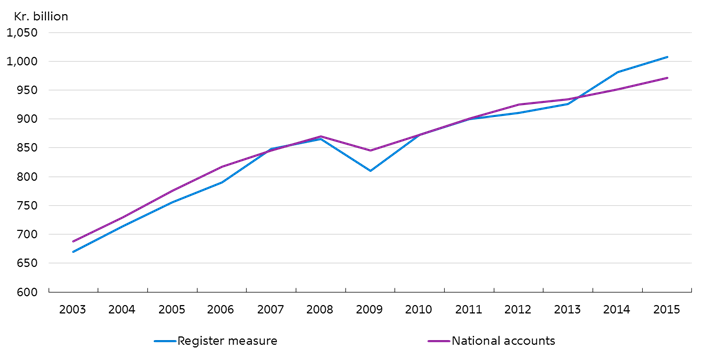
\includegraphics[scale=0.8]{\econtexRoot/Figures/consumption_measures.png} 
		\caption{Imputed Register Measure and National Account Measure of Expenditure (from \cite{abildgren_consistency_2018})}
		\label{fig:ConsumptionMeasures}
	\end{centering}
\end{figure}

\subsection{Sample Selection}
As our methodology requires income uncertainty to be relatively constant through the observed period and the young and old are likely to have predictable income trends unobservable to the econometrician, we limit the sample to households headed by an individual between the ages of 30 and 55 in 2008.\footnote{Online appendix \ref{sample_selection} shows the assumption holds for this age group.} Our final sample contains 7.7 million observations from 2004 to 2015 from an age group population totaling 18.1 million. The selection criterion that reduces the sample size the most is the requirement that a household does not make a housing transaction for a period of five years. Table \ref{table:SummaryStatistics} shows summary statistics for all Danish households whose head fits into this age group as a whole as well as the sample we use in estimation. It is reassuring that both the mean and median values for after-tax income and consumption are similar in the estimation sample and the population. Our estimation sample has much lower standard deviations as a mechanical result of excluding the top and bottom 1\% of the income and consumption distributions that contain extreme values. Sample selection shows up in homeownership and car ownership, as we exclude those households that buy a house at the end of a five year period but who otherwise would be counted as renters. As a result, our sample is, on average one year older than the population. Unhedged Interest Rate Exposure (URE) and Net Nominal Position (NNP) will be discussed in section \ref{monetary_policy}, but again the significant differences here are due to the housing transaction criteria. 
\begin{center} 
	\begin{table}
		\caption{Summary Statistics}
	%\captionof{table}{Summary Statistics}
	\label{table:SummaryStatistics}
	\input\econtexRoot/Tables/summary_statistics.tex 
	\end{table}
\end{center}

\section{Income and Consumption Characteristics by Household Wealth} \label{MPX_wealth}
Liquidity constraints are the key microfoundation for the lack of consumption smoothing in heterogeneous agent models. In this section we look at the empirical relation between liquid wealth and the marginal propensity to expend (MPX) out of both permanent and transitory shocks to income. We find a strong monotonic negative relation. We also look at net wealth and find such a monotonic relation no longer holds.

Using our entire estimation sample we find a mean MPX out of transitory shocks of 0.50 and a mean MPX out of permanent shocks of 0.72. However, these averaged results hide a significant amount of heterogeneity. From the standpoint of consumption theory it is the ability of households to self-insure with their own wealth that mostly determines how much they smooth their consumption over shocks. We divide our estimation sample into quintiles according to both liquid wealth (which we define as bank deposits\footnote{The results are little changed using any other definition of liquid wealth as long as housing and debts are excluded. See online appendix \ref{robustness}.}) and net wealth. In each case, wealth is measured as the mean household wealth holdings over the entire sample period.
\begin{figure}
	\centering
	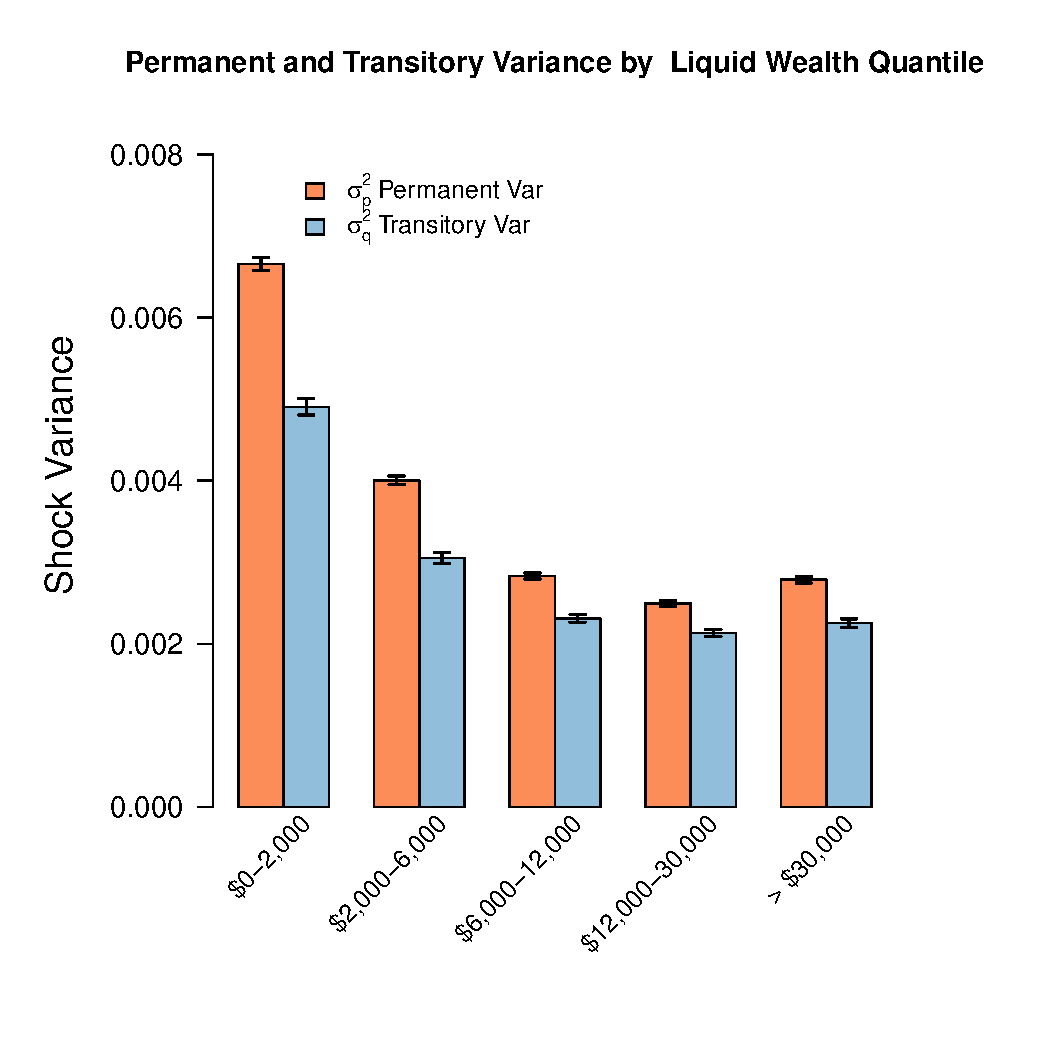
\includegraphics[scale=0.4]{\econtexRoot/Figures/VarianceByLiquidWealth_level_lincome_head.pdf}
	\centering
	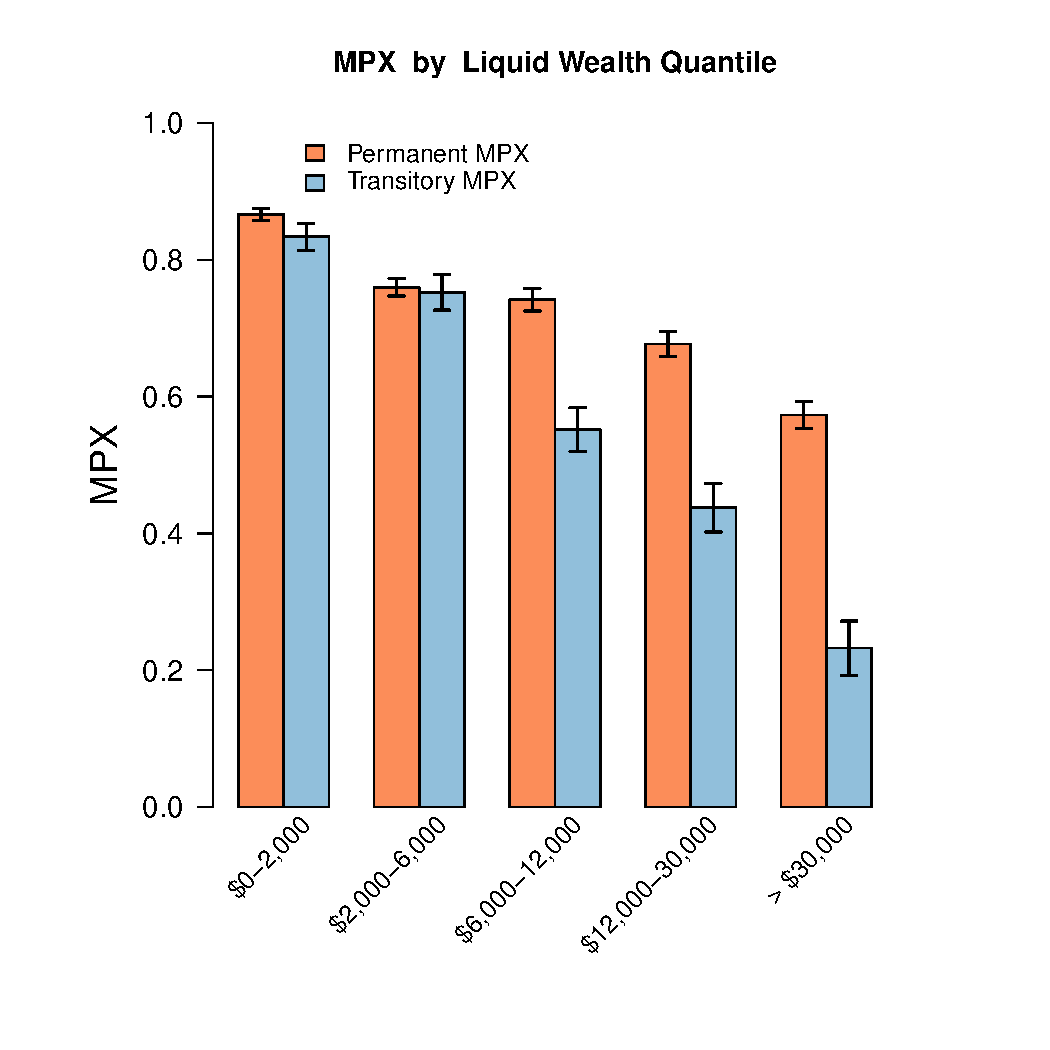
\includegraphics[scale=0.4]{\econtexRoot/Figures/MPXByLiquidWealth_level_lincome_head.pdf}
	\caption{Variance and MPX by Liquid Wealth Quintile}
	\label{fig:MPXByLiquidWealth}
\end{figure}

Figure \ref{fig:MPXByLiquidWealth} shows the estimated income variances and MPXs for households in each quintile of liquid wealth.\footnote{For these graphs, and all similar ones in this paper, the 95\% confidence intervals are shown above and below each quantile estimate.} Looking at the left-hand variance panel first, it is noticeable that income uncertainty, and particularly permanent income uncertainty, is highest for households in the lowest quintile of liquid wealth. This low buffer-stock, despite high income volatility, provides some evidence towards the idea that heterogeneous tastes (e.g. discount factors of risk aversion) may be more important than income risk in determining wealth held for precautionary saving. For households in the top three quintiles of liquid wealth, the similarity of their level of income risk is remarkable. Note that in contrast to standard estimates of the U.S. income process, permanent income variance in Denmark is slightly higher than transitory variance, likely due to the high levels of social insurance available in Denmark. The variance level, at just over 0.002 for these top three quintiles, represents a standard deviation of just below 5\% of permanent income per year.

Note that the estimates of income variance we obtain are highly sensitive to our treatment of outliers, but our MPX estimates do not change.\footnote{See online appendix \ref{robustness} for evidence of this.}

The right-hand panel of figure \ref{fig:MPXByLiquidWealth} shows our estimates for the MPX out of permanent and transitory shocks by liquid wealth quintile. The lowest wealth quintile, who hold less than \$2,000 in bank deposits on average over the sample period, look somewhat like hand-to-mouth consumers. They respond almost equally to permanent and transitory shocks, spending over 80\% of income shocks in the year that it arrives. However, the fact that both permanent and transitory MPXs are very similar and significantly less than 1 suggests that these households may be more accurately modeled as saving in an illiquid asset such as housing or a pension following a rule of thumb (say, 20\% of income) and then living hand to mouth on the remainder. As the quintile of liquid wealth increases, the MPX out of both transitory and permanent income decreases. In the top quintile, formed of households that maintained a mean bank balance above \$30,000, the MPX out of permanent shocks is 0.57 and out of transitory shocks 0.23. From the point of view of theory, the responsiveness of spending out of permanent shocks in this quintile is low, while that of transitory shocks is high.
\begin{figure}
	\centering
	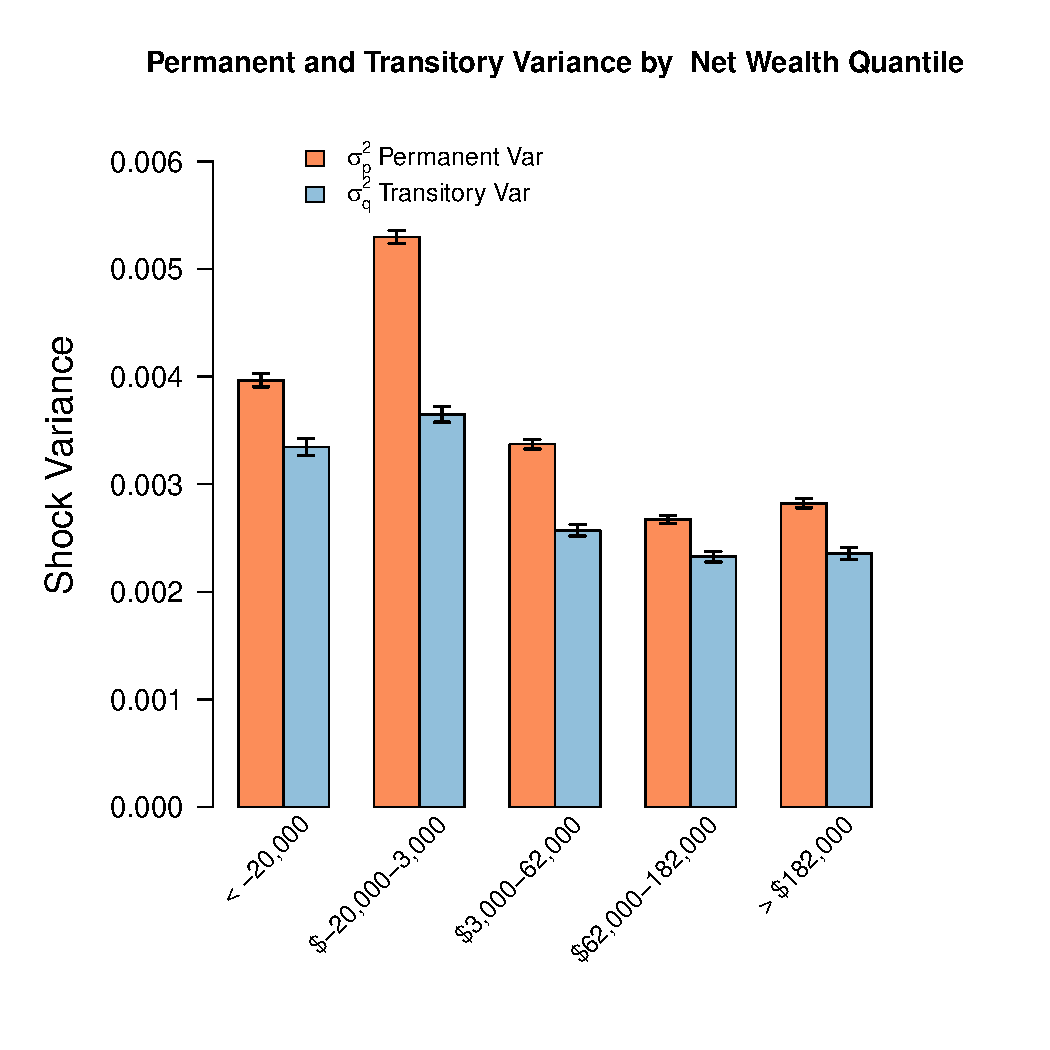
\includegraphics[scale=0.4]{\econtexRoot/Figures/VarianceByNetWealth_level_lincome_head.pdf}
	\centering
	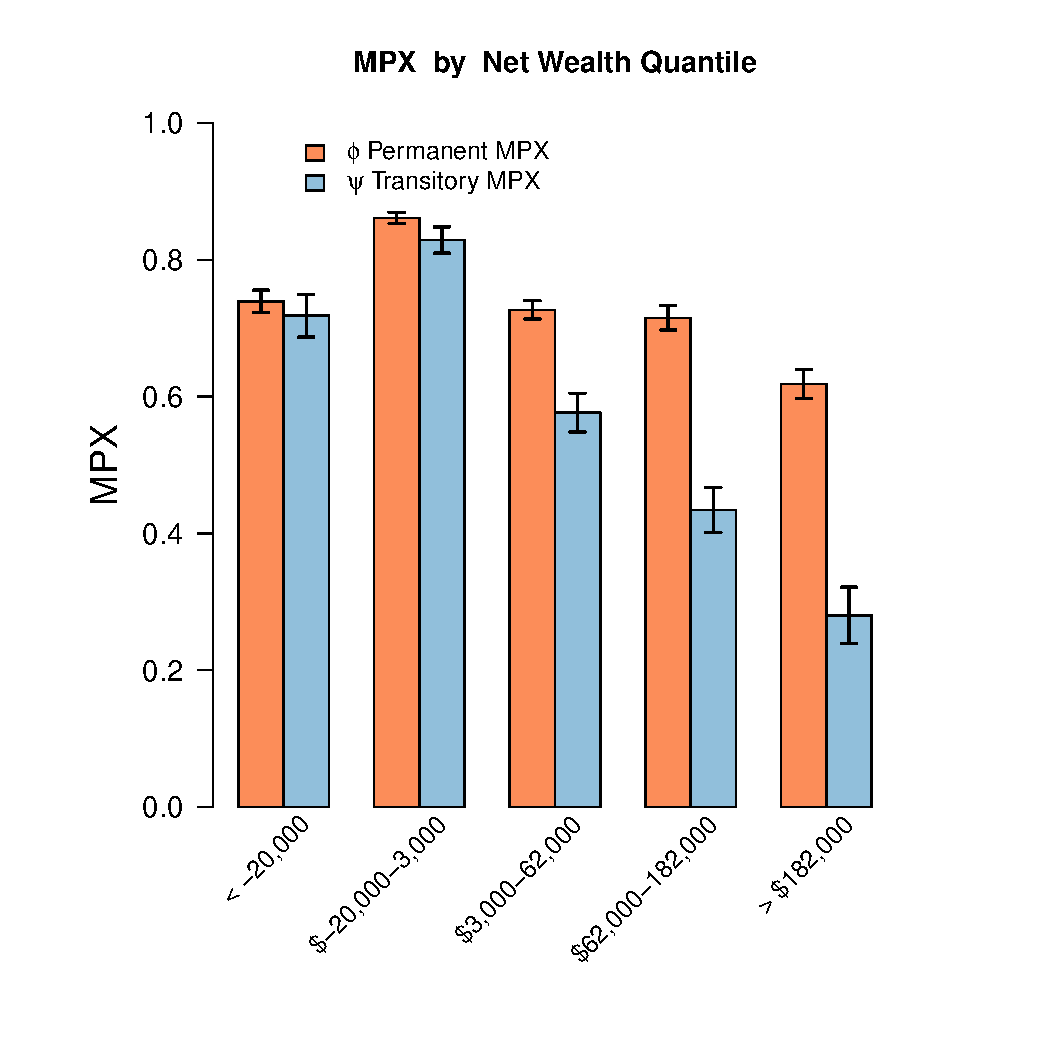
\includegraphics[scale=0.4]{\econtexRoot/Figures/MPXByNetWealth_level_lincome_head.pdf}
	\caption{Variance and MPX by Net Wealth Quintile}
	\label{fig:MPXByNetWealth}
\end{figure}

Figure \ref{fig:MPXByNetWealth} shows the estimates for households grouped by quintiles of net wealth. Here the pattern is slightly different. The quintile with the highest MPX out of both transitory and permanent income is the second lowest, the quintile that contains zero net worth. Households in the lowest quintile---those with over \$20,000 in net debt---do not seem to distinguish between permanent and transitory income shocks in their consumption responses, but their MPX for both is about 10 percentage points lower than the quintile with close to zero net wealth. The pattern for quintiles 3 to 5 looks similar to that for liquid wealth: the MPX out of transitory shocks falls sharply to around 0.28, while that out of permanent shocks also falls but more slowly to 0.62.

These results are broadly in line with the literature. The population mean of 0.5 for transitory MPX is a little higher than most estimates from table \ref{table:MPCLiterature}, but, bearing in mind that our estimate includes durables and is best compared to a six-month MPC, it is certainly not an outlier. The MPX out of permanent shocks of 0.72 is also between the BPP estimate of 0.65\footnote{The permanent ``insurance'' coefficient estimated by BPP does not suffer as much from the time aggregation problem as the transitory coefficient.} and the estimate of 1.0 from \cite{gelman_response_2016}. The strength of the relationship between liquid wealth and MPC is similar to that found in \cite{gelman_what_2016} and stronger than in \cite{fagereng_mpc_2016}.

\section{Monetary Policy and the Redistribution Channel} \label{monetary_policy}
\cite{auclert_monetary_2017} lays out a clear and intuitive theory as to how heterogeneity in the MPC out of transitory shocks affects the transmission mechanism of monetary policy. He identifies five channels through which monetary policy can act, three of which are absent without heterogeneity.\footnote{The key assumption made to link MPC with monetary policy redistribution is that households respond to redistribution in the same way as a transitory shock to income. We believe this is a reasonable assumption for the interest rate exposure channel, where households will have to pay a higher or lower rate out of liquid assets, but perhaps not for the Fisher channel. If the price level goes up 1\%, a \$100,000 debt is made smaller by \$1,000 in real terms. However, the liquidity position of the household with this debt is not changed. As a result, we have reservations about the reliability of our estimate of the size of the Fisher channel, which we estimate to be very large.} He then uses this theory to identify a small set of sufficient statistics that help distinguish which of these channels are of quantitative importance.

While these statistics in theory are highly informative about the transmission mechanism of monetary policy, good data and MPC estimation methods are required to estimate them convincingly. Auclert states, ``As administrative quality household surveys become available and more sophisticated identification methods for MPCs arise, a priority for future work is to refine the estimates I provide here.'' We are able to bring our new MPC estimation method, along with administrative data from Denmark, in order to estimate Auclert's sufficient statistics.

Our data have two significant advantages over previous efforts.\footnote{As well as \cite{auclert_monetary_2017}, a new version of \cite{fagereng_mpc_2016} also attempts to estimate these statistics.} First, our sample size is very large, containing a large percentage of all households in Denmark. Second, we have detailed balance sheet information for not only households within our sample, but also for those excluded from our sample. Furthermore, we are able to identify interest rate risk and nominal positions held by firms, foreigners, and the government so that the aggregate position is zero, as required in equilibrium, and allows us to avoid some problematic assumptions otherwise needed for aggregation of household data.

\subsection{Distribution of Marginal Propensity to Expend (MPX) Across NNP, URE, and Income}
The redistribution effects of monetary policy depend crucially on two household characteristics, their Net Nominal Position and Unhedged Interest Rate Exposure.
\begin{itemize}
	\item \textbf{Net Nominal Position (NNP)} is the net value of a household's nominal assets and liabilities. It's relevance for analyzing the redistributive effects of monetary policy comes from the fact that an unexpected rise in the price level will decrease the wealth of households with positive nominal assets, redistributing it to those with negative NNP (who now have less real debt). In administrative data we are able to observe directly held nominal positions at the household level, including bank deposits and loans, bond holdings, and mortgages. In aggregate, the directly held NNP position of the household sector is negative, which from the national accounts we will see is balanced by the financial sector as well as foreigners.
	\item \textbf{Unhedged Interest Rate Exposure (URE)} measures the total amount that a household plans to save at the going interest rate during that period. It is the difference between all maturing\footnote{We define ``maturing'' assets and liabilities as those that are due to have their interest rates reset, even if they contractually exist for a longer period. For example, a 30 year variable rate mortgage with annual interest rate fixation periods is ``maturing'' each year in our definition.} assets (including income) and liabilities (including planned consumption). For example, households with a large variable rate mortgage will likely have very negative URE. For these households, the entire value of their mortgage will be adjusted to the new rate. When the interest rate rises for one period they will see their disposable income (after mortgage payments) go down, and hence if they have a high MPX their spending will also decrease. To calculate URE we assume all bank deposits and bank debt to have a variable rate that changes instantaneously. For mortgage debt we directly observe the amount resetting over the following year and assume that the new rate will only apply for half of the year.\footnote{See online appendix \ref{mortgage_market} for more details on the Danish mortgage market. Note that the prevalence of fixed-rate mortgages will strongly influence the distribution of URE. To the extent that the United States has more fixed-rate mortgages than Denmark, the interest rate exposure channel is likely to be smaller in the United States. Furthermore, household debt to income is about twice as large in Denmark as the United States. A detailed examination of the Survey of Consumer Finance would be a valuable exercise in determining the likely differences.} For all other assets and liabilities we assume a maturity of five years. As with NNP we find households on aggregate have a negative URE position in our data, and this is counterbalanced by the interest rate position of the financial sector. See online appendix \ref{URE_NNP_appendix} for more details on how we calculate NNP and URE positions.
\end{itemize}

Figure \ref{fig:MPCAuclert} shows how the MPX varies across household values for URE, NNP, and income. In each case, the value on the x-axis has been divided by the mean level of expenditure of the entire sample. The top chart shows the estimated MPX for each decile of unhedged interest rate exposure. The deciles on the left contain households most negatively exposed to a rise in interest rates, those in the middle deciles have little exposure, while the two top deciles on the right have the most to gain from an interest rate rise. We have included in this figure data on both rates of homeownership and median liquid assets for each decile. A clear pattern emerges in which we can roughly categorize the deciles into three groups following \cite{violante_wealthy_2014}:
\begin{itemize}
	\item \textbf{Wealthy Hand-to-Mouth:} The first five deciles contain households with high levels of homeownership but relatively few liquid assets. These households have relatively high MPXs, and it is likely that their wealth is locked up in illiquid assets (mostly housing) and that they have large mortgages.
	\item \textbf{Poor Hand-to-Mouth:} The next three deciles tend to be renters with very little in the way of liquid assets either. These households have very high MPXs and are close to being truly hand-to-mouth. As they have few assets, they have very little exposure to interest rates and cannot easily substitute consumption between periods; therefore, their consumption behavior is likely not affected by changes in interest rates directly.\footnote{Neither the interest rate exposure channel nor the intertemporal substitution channel will have much impact on their consumption. Monetary policy could impact their expenditure strongly through income effects.}
	\item \textbf{Wealthy:} The top two deciles contain households that are both likely to be homeowners and hold very large liquid asset balances. These are likely to be households that own their house outright without a mortgage and have been able to build up a large stock of liquid assets. Relative to the other deciles they have low MPX and are likely able to use their assets to effectively consumption smooth.
\end{itemize}

The distribution of MPX with net nominal position follows a similar pattern. As mortgages in Denmark are a mixture of fixed and variable rates (see online appendix \ref{mortgage_market} for details on the Danish mortgage market), we can think of a typical household with negative URE or NNP as having a large mortgage, while those with positive URE or NNP are wealthy households with lots of liquid wealth. This pattern has not been evident in previous attempts to measure the distribution of MPX across these dimensions. Most importantly for the theory, the average MPX for those with negative URE and NNP positions is significantly greater than for those with positive URE or NNP. Note that the mean levels of both URE and NNP are negative for the households in our estimation sample, so even a constant (positive) MPX would result in interest rate hikes reducing their expenditure if not balanced by indirectly held exposures.\footnote{In contrast, \cite{auclert_monetary_2017} finds a mean positive URE across households. We believe the difference is partly due to the prevalence of fixed-rate mortgages in the United States, but also due to underreporting of expenditures, especially in the PSID data.}

The final chart in figure \ref{fig:MPCAuclert} shows the distribution of MPX with total household income. There is a clear downward trend. If the income of lower-income households decreases more than that of high-income households during a monetary policy contraction, then expenditure will go down by more than the mean income-weighted MPX that would be the result of a representative agent model.

For comparison, the distribution of  MPX out of permanent income shocks across these three dimensions can be found in online appendix \ref{PermMPXbyURENNP}.
\begin{figure} 
\begin{centering}
	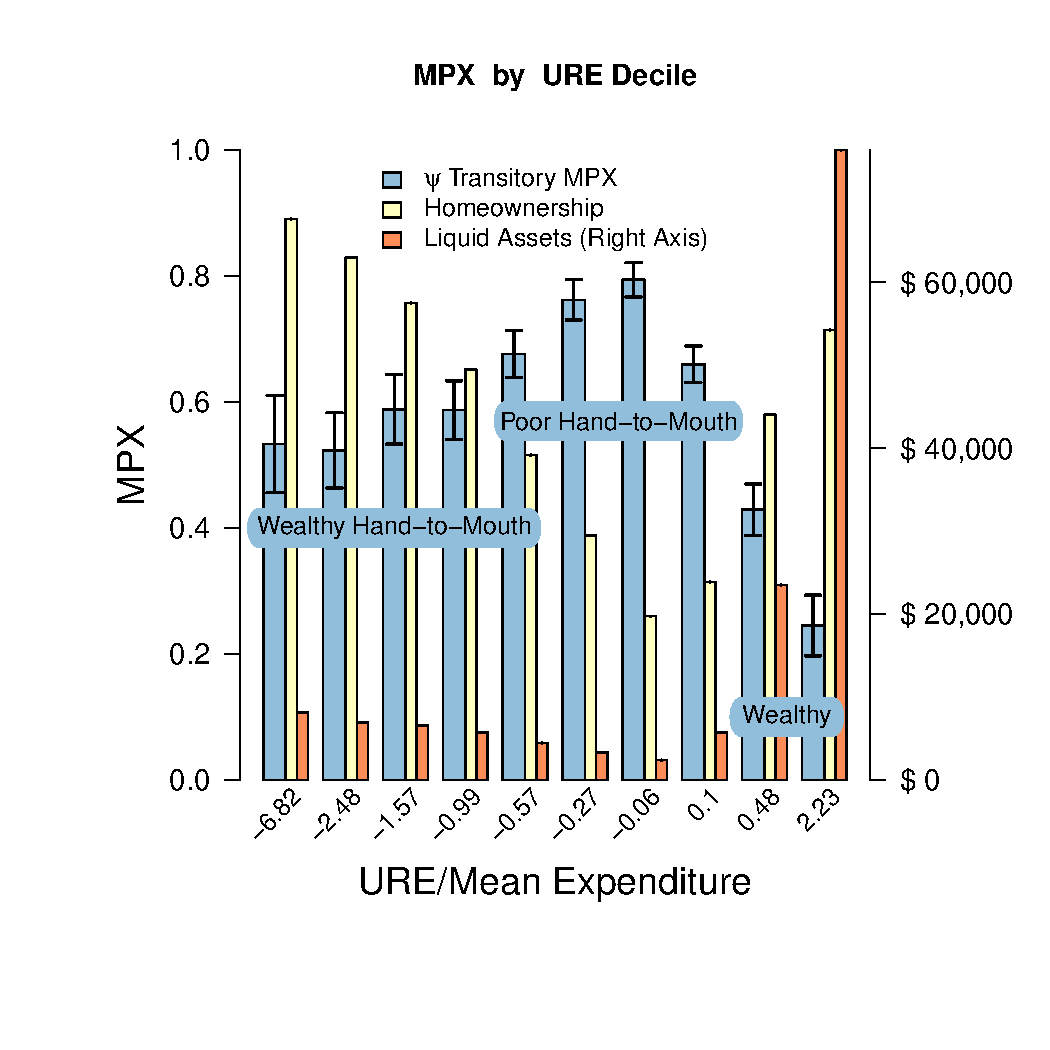
\includegraphics[scale=0.85]{\econtexRoot/Figures/MPXByUREdetailsPaper_level_lincome_head.pdf} \\
	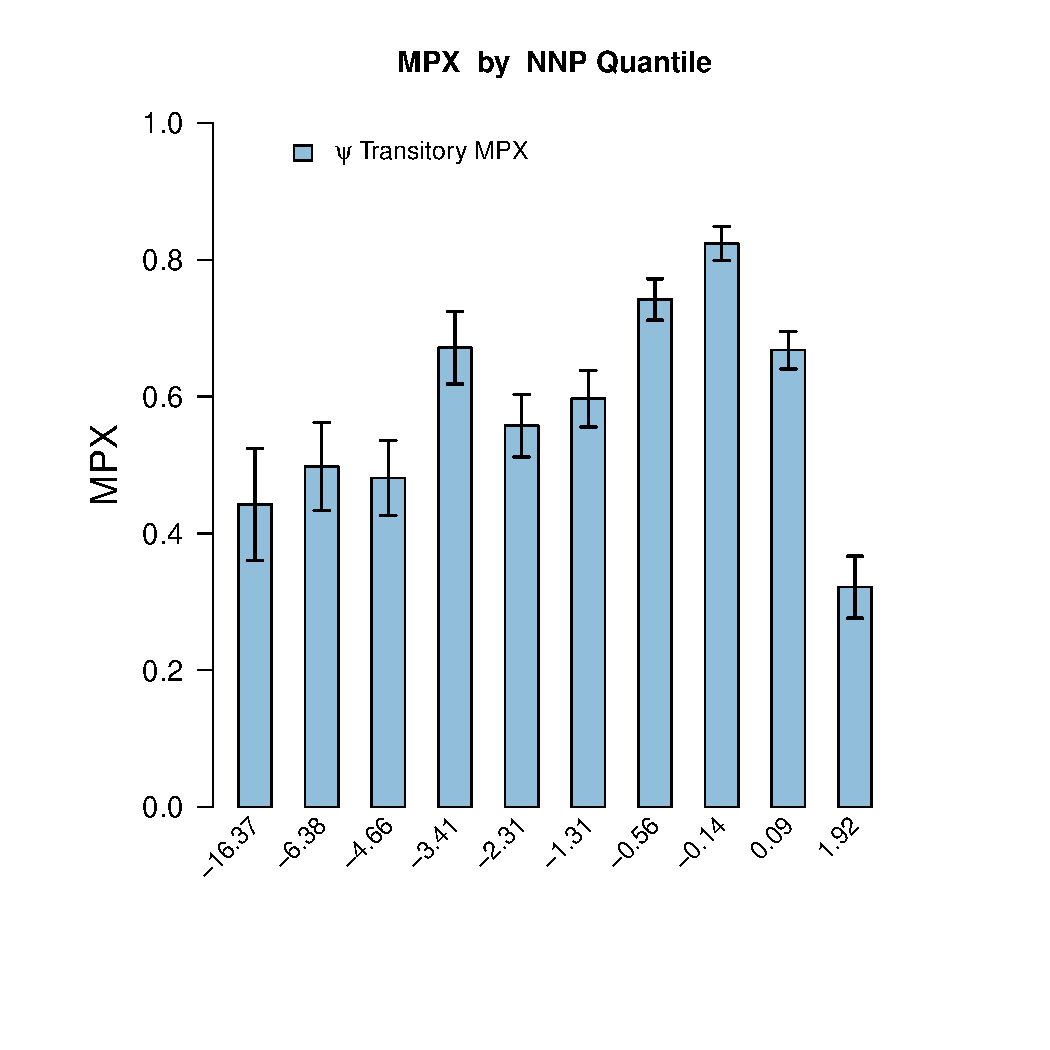
\includegraphics[scale=0.4]{\econtexRoot/Figures/MPXByNNP_level_lincome_head.pdf}
	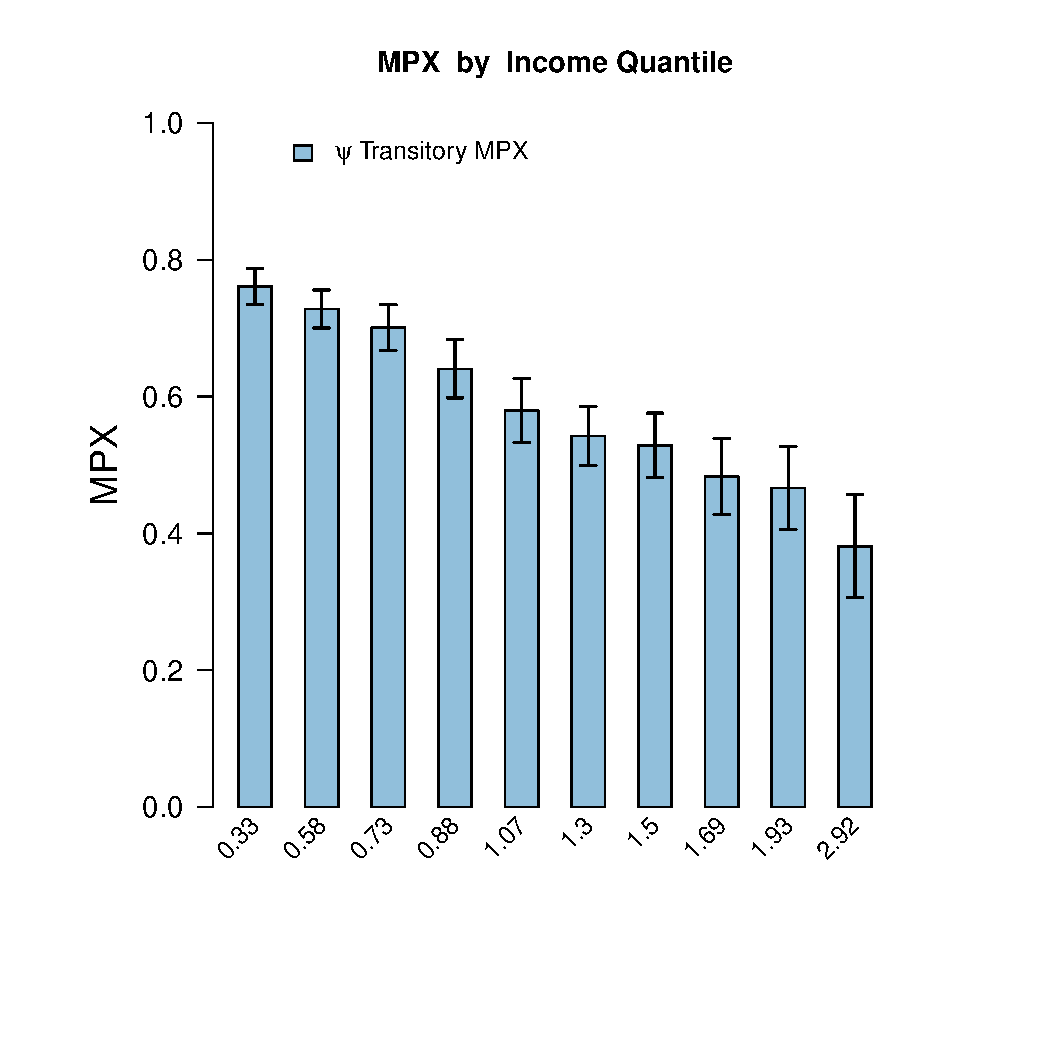
\includegraphics[scale=0.4]{\econtexRoot/Figures/MPXByIncome_level_lincome_head.pdf}
	\caption{MPX Distribution by URE, NNP, and Income}
	\label{fig:MPCAuclert}
\end{centering}
\end{figure}

\subsection{Theoretical Setup and Sufficient Statistics}
Auclert's method is to consider individual households' consumption response to a monetary policy shock in which (i) the real rate of interest changes for one period by $dR$, (ii) the price level makes a one-time change of $dP$ and then remains at the new level, and (iii) aggregate income makes a transitory change of $dY$. While the dynamics here are clearly stylized, and in particular lack any lag in the economy's response, we believe such a simple experiment to be highly informative as to the relative sizes of each transmission channel.

\cite{auclert_monetary_2017} divides the effect of monetary policy on aggregate consumption into five distinct channels:
\begingroup
\allowdisplaybreaks[0]
\begin{align} 
\frac{dC}{C} &= \overbrace{\mathcal{M}\frac{dY}{Y}}^{\text{Aggregate Income Channel}\qquad} \overbrace{ + \gamma \mathcal{E}_Y \frac{dY}{Y}}^{\text{Earnings Heterogeneity Channel}\qquad} \overbrace{ - \mathcal{E}_P\frac{dP}{P}}^{\text{Fisher Channel}}  \nonumber \\
& \qquad \underbrace{ + \mathcal{E}_R \frac{dR}{R}}_{\text{Interest Rate Exposure Channel}\qquad}  \underbrace{ - \sigma \mathcal{S}\frac{dR}{R}}_{\text{Intertemporal Substitution Channel}} \label{auclert_channels}
\end{align}
\endgroup
where $\sigma$ is the elasticity of intertemporal substitution, $\gamma$ is the elasticity of relative income to aggregate income\footnote{Here we are making the simplifying assumptions that these quantities are common for all households; see \cite{auclert_monetary_2017} for a discussion.} and the five sufficient statistics, $\mathcal{M}$, $\mathcal{E}_Y$, $\mathcal{E}_P$, $\mathcal{E}_R$, and $\mathcal{S}$, are measurable in the data and defined in table \ref{table:auclertSS}. We choose to define these statistics to include the consumption effects coming from exposures not directly held by households. We allocate the aggregate URE and NNP exposure from our estimation sample into seven bins so that the total exposure across the economy is zero. These bins include households with (i) young (<30) and (ii) old (>55) heads, and exposures held by households indirectly through (iii) pension funds, (iv) government, (v) nonfinancial corporates, (vi) financials, and (vii) exposures held by the rest of the world. Within each of these bins we assume no heterogeneity so that the MPX with respect to these exposures is constant. This assumption is conservative, and likely underestimates the size of the heterogeneous agent channels. Our assumptions on the level of these MPXs can be seen in table \ref{table:aggElas}.

\begin{minipage}{1.0\textwidth}
	\begin{center}
%		\begin{table}
%			\caption{Sufficient Statistics Definitions}
		\captionof{table}{Sufficient Statistics Definitions}
		\label{table:auclertSS}
		\resizebox{\textwidth}{!}{\begin{tabular}{ccl}
			\textbf{Statistic} & \textbf{Definition} & \textbf{Description} \\
			\hline
			$\mathcal{M}$ & $\frac{1}{C}\Bigg[ \sum\limits_{i \in \text{Income deciles} } \text{MPX}_i Y_i + \sum\limits_{j \in \{\text{young,old}\}} \text{MPX}_j Y_j \Bigg]$ & Income-weighted MPX \\
			$\mathcal{E}_Y$ & $\mathcal{M} - \overline{\text{MPX}}\frac{Y}{C}$ & Redistribution elasticity for Y \\
			$\mathcal{E}_P$ & $\frac{1}{C}\Bigg[ \sum\limits_{i \in \text{NNP deciles} } \text{MPX}_i \text{NNP}_i + \sum\limits_{j \in \text{bins}} \text{MPX}_j \text{NNP}_j \Bigg]$ & Redistribution elasticity for P \\
			$\mathcal{E}_R$ & $\frac{1}{C}\Bigg[ \sum\limits_{i \in \text{URE deciles} } \text{MPX}_i \text{URE}_i + \sum\limits_{j \in \text{bins}} \text{MPX}_j \text{URE}_j \Bigg]$ & Redistribution elasticity for R \\
			$\mathcal{S}$ &$1-\frac{1}{C}\Bigg[ \sum\limits_{i \in \text{Consumption deciles} } \text{MPX}_i C_i + \sum\limits_{j \in \{\text{young,old}\}} \text{MPX}_j C_j \Bigg]$ & Hicksian scaling factor \\
			\hline
		\end{tabular}}
	\tiny \textbf{Note: } $\overline{\text{MPX}}$ is the mean MPX over all households in the economy. $Y$ and $C$ are aggregate household income and consumption respectively. Bins refers to the seven categories for which we have allocated URE and NNP exposures outside our estimation sample. \{young,old\} are the two bins that contain young and old households (the other five bins are only relevant for URE and NNP exposures as $Y$ and $C$ measure \textit{household} income and consumption).\\
%\end{table}
\end{center}
\end{minipage}


We define $\mathcal{E}_R$ as
\begin{align}
\mathcal{E}_R = \frac{1}{C}\Bigg[ \sum_{i \in \text{URE deciles} } \text{MPX}_i \text{URE}_i + \sum_{j \in \text{bins}} \text{MPX}_j \text{URE}_j \Bigg]
\end{align}
where $i$ sums over the 10 deciles of URE, $j$ over the seven bins defined above, and $C$ is aggregate household expenditure in the economy. This method of dealing with the fact that aggregate exposure does not equal zero in the estimation sample is different to the approach taken by Auclert. He assumes the residual exposure is distributed equally across households in the sample. By making use of the national accounts, we believe we are able to get a better handle on the likely MPXs to attach to this residual exposure. Table \ref{table:auclertSS} shows the definitions we use for each of the five measurable statistics in equation \ref{auclert_channels}.


\subsection{Out of Sample Marginal Propensity to Expend (MPX)}
The assumptions we make about the MPX of the young and the old, as well as out of indirectly held URE and NNP exposures, are shown in table \ref{table:aggElas}. In each case we believe we have made conservative choices that will underestimate the size of the interest rate exposure channel of monetary policy. For the young we choose an MPX of 0.5, in line with the rest of the population. As the young have aggregate negative exposures, choosing an MPX on the low side is conservative. Similarly, for the old we choose an MPX of 0.5, which is on the high side for this age group. The assumption that there is no heterogeneity in MPX within these groups is also a very conservative assumption.

\begin{center}
	\begin{table}
		\caption{Aggregating Redistribution Elasticities}
	%\captionof{table}{Aggregating Redistribution Elasticities}
	\label{table:aggElas}
	\input ./Tables/URE_NNP_table.tex
	\end{table}
\end{center}

Much of the URE and NNP exposure is not held directly on the balance sheet of households but instead indirectly through pension funds, corporates, and the government. There is significant evidence that the MPX out of shocks to the value of pension wealth, stocks, or the government balance sheet is substantially lower than the MPX from income. We choose to use the estimate from \cite{maggio_stock_2018} that households' MPX from changes in stock market wealth is about 10\%. This choice is the most quantitatively important, as the bin containing the most exposure is the financial sector, which is positively exposed to interest rate increases. This positive interest rate exposure may seem surprising as banks are typically thought to have long-term assets and short-term debt that would result in negative URE exposure. However, our findings are in line with \cite{landier_banks_2013}, who find that the aggregate financial sector benefits from interest rate hikes, although there is a large amount of heterogeneity between different banks. An important caveat is due here: we focus on the MPX out of changes in the assets indirectly held by households through the financial sector and do not assume any spending or lending response at the bank level. This assumption may be reasonable in good times when banks are not credit constrained, but will not be the case during a banking crisis. Financial frictions could possibly result in monetary policy being much less effective during a banking crisis as the interest rate exposure channel to household spending is counterbalanced by a channel from bank balance sheet interest rate exposure to lending.\footnote{It should be noted that our analysis is all on the household side. Evidence suggests that firms are also sensitive to changes in cash flow; for example, see \cite{blanchard_what_1994}.} 

We choose an MPX of zero for government and the rest of the world. There is no evidence that households respond in any significant way to changes in the government's balance sheet, and furthermore a low MPX is a conservative assumption for the size of the heterogeneous agent channels. As Denmark is a very small part of the world economy we assume that foreigners spend a negligible proportion of their wealth there.

\subsection{Results}
Our estimates of the five sufficient statistics, along with their standard errors, are shown in table \ref{table:suff_stats}. The aggregate income channel is summarized by $\mathcal{M}$ that we estimate to be 0.52. This means that if income for all households in the economy increased by 1\%, aggregate consumption would increase by 52 basis points, broadly in line with calibrations of saver-spender models designed to fit evidence from \cite{campbell_consumption_1989}. We find little role for the redistribution effect of income, $\mathcal{E}_Y$, despite the clear negative correlation between income and MPX seen in figure \ref{fig:MPCAuclert}.\footnote{\cite{patterson_2019} finds a larger role for income heterogeneity by dividing households into groups that have differing income sensitivity to aggregate income.} $\mathcal{S}$, the Hicksian scaling factor, is 0.49, which reduces the size of the intertemporal substitution channel by close to half.

The two most interesting statistics are $\mathcal{E}_P$ and $\mathcal{E}_R$, both of which act through redistribution from households with low MPX to those with high MPX. $\mathcal{E}_P$ is estimated to be  negative 0.75 suggesting that a one-time increase in the price level of 1\% increases aggregate consumption by 75 basis points due to redistribution from those with large nominal assets to those with large nominal debts. This Fisher channel of monetary policy is emphasized in \cite{doepke_inflation_2006}. The interest rate exposure channel is also large. We estimate  $\mathcal{E}_R$ to be  negative 0.26, suggesting that a 1\% increase in the interest rate decreases expenditure by 26 basis points.\footnote{These estimates are significantly different to the results found in \cite{auclert_monetary_2017}. Our estimate of the Fisher channel is an order of magnitude larger, while our estimate of the interest rate exposure channel is over twice as large.}

For both of these channels, but particularly the interest rate exposure channel, it is informative to compare them to the size of the intertemporal substitution channel. An increase in the real interest rate reduces aggregate consumption today by $\sigma \mathcal{S}$ multiplied by the percent change in the rate where $\sigma$ is the intertemporal elasticity of substitution. Reliable estimates of $\sigma$ have been elusive to the economics profession, but there is very little evidence of a large positive number. \cite{havranek_measuring_2015} provides a meta-study of the elasticity of intertemporal substitution and finds a mean of zero from studies using macrodata, and 0.3 to 0.4 for those using microdata. Many of these microlevel studies suffer from identification problems.\footnote{See \cite{carroll_death_2001} for a critique of many older studies of the elasticity of intertemporal substitution.} \cite{best_estimating_2018} make use of mortgage notches in the United Kingdom to overcome some of these problems. They estimate the average elasticity of intertemporal substitution to be 0.1, which would result in a size of the intertemporal substitution channel of monetary policy being 0.05, over five times smaller than our estimate of the interest rate exposure channel.\footnote{Our decomposition does not allow easy comparison of the interest rate exposure channel with the aggregate income channel, as we do not make assumptions about how much aggregate income changes. \cite{cloyne_monetary_2016} compare mortgagors with outright homeowners and find the aggregate income channel is larger than the direct effect of higher mortgage payments.}
\begin{center}
	\begin{table}
		\caption{Sufficient Statistics}
	%\captionof{table}{Sufficient Statistics}
	\label{table:suff_stats}
	\begin{center}
	\input ./Tables/sufficient_stats.tex
	\end{center}
	\end{table}
\end{center}
A long outstanding question in monetary economics is why monetary policy acts with a lag. Two competing theories are habits models such as \cite{fuhrer_habit_2000} and sticky information models such as \cite{mankiw_sticky_2002}. \cite{carroll_sticky_2018} find evidence toward the idea that households react fast to their own idiosyncratic income shocks, but news about macroeconomic shocks takes time to be absorbed. A possible third alternative to both of these theories is that households respond strongly to their realized income today, but not to income anticipated in the future. As it takes time for variable rate mortgages to reset (typically from six months up to five years in Denmark), this would result in the interest rate exposure channel acting with a delay. Indeed, the literature on consumption responses to transitory income shocks has generally found little difference between anticipated and unanticipated responses. Many of the estimates in table \ref{table:MPCLiterature} use anticipated shocks (such as tax rebates) as an instrument and find large MPCs, suggesting households do not necessarily pay attention to anticipated cash flows until they arrive. \cite{ganong_consumer_2017} show this very clearly: there is a sharp consumption drop in the month that unemployment benefits expire, an entirely anticipated event. A model that takes these results seriously, along with a large role for the interest rate exposure channel of monetary policy, could be a fruitful area for future research. 

\section{Threats to Identification}
\label{threats_to_identification}
In the online appendix we address a number of identification concerns.\footnote{Online appendix \ref{Consumption_persistence} looks a consumption persistence beyond two years; \ref{durables_appendix} goes into more detail on durables; \ref{rip_hip_appendix} considers alternative income processes; \ref{time_varying_risk} looks at time-varying risk; and \ref{robustness} looks at alternative data definitions.} Here we focus on two that we think deserve highlighting: measurement error and durable expenditure.

\subsection{Measurement Error} \label{Measurement_error}
Our identification comes from estimating $\mathrm{Var}(\Delta^N \bar{y})$ and $\mathrm{Cov}(\Delta^N \bar{c},\Delta^N \bar{y})$ using our observed data. For unbiased estimates of $\mathrm{Var}(\Delta^N \bar{y})$ we require no measurement error in our observed changes in labor income. For unbiased estimation of $\mathrm{Cov}(\Delta^N \bar{c},\Delta^N \bar{y})$ we only require (further to no measurement error in income growth) that the measurement error in expenditure growth is uncorrelated with labor income growth. As our expenditure is imputed from income and changes in assets, this is potentially more of a concern than would be the case in survey data in which questions about consumption are not directly linked to those on income. We will examine potential sources of error in labor income and imputed consumption.

\subsubsection{Labor Income}
For most workers, labor income is well measured. Third party reporting, along with a high level of trust in government institutions, means that underreporting is likely very low. The black economy in Denmark is small, and to the extent that any growth in unreported income is uncorrelated with growth in reported income this will not bias our estimates.\footnote{Such income may show up as a change in net wealth and hence expenditure, but measurement error in the change in expenditure uncorrelated with the change in labor income will not bias our MPX estimates.} In contrast to survey data, in which measurement error in income is likely to downwardly bias transitory MPX estimates, this is of very little concern in our data.

\subsubsection{Imputed Expenditure}
Expenditure is calculated as the residual of total household income (including interest and dividends) after pension contributions and the change in net wealth have been deducted. For households with simple financial lives (which we believe fits most of the Danish population), this should work well. There are a few scenarios that merit further investigation.
\begin{itemize}
	\item \textbf{Stock Market Capital Gains:} Only 10\% of Danish households directly own stocks or mutual funds.\footnote{In our calculation we directly observe flows in and out of pension accounts, so these can be treated as off balance sheet in which capital gains do not affect our expenditure calculation.} In online appendix \ref{robustness} we show that the qualitative patterns we observe are unchanged even when we completely remove these households from the sample. For households that do own stocks, we assume the return they receive is equal to a diversified portfolio of Danish stocks. Given that different households will have their own idiosyncratic portfolios, this methodology will result in significant measurement error. \cite{baker_measurement_2018} show that the size of this measurement error is not only correlated with income and wealth, but also with the business cycle. Furthermore, \cite{fagereng_persistence_2016} show that some groups of investors consistently outperform the market, which would lead us to consistently underestimate their expenditure. Our concern, however, is that the \textit{change} in measurement error of expenditure be correlated with the \textit{change} in labor income. Consistently underestimating expenditure by the same amount is therefore not a problem for us. Furthermore, as we have removed all aggregate effects from the labor income residuals that we use in estimation, any measurement error correlated with the business cycle will be uncorrelated with our measure of changes in labor income. We see two potential ways in which mis-measuring stock returns may bias our results. First, if households have significantly invested in the stock of the firm they work for, which is likely only to be the case for high-level management. Second, to the extent that households invest their labor income gains halfway through the year, we will underestimate expenditure for those whose income increases, and overestimate it for those whose income decreases, leading us to underestimate the MPX. The size of this bias is limited by the size of excess expected returns, so our MPX estimate will be biased by no more than a few percentage points.
	\item \textbf{Family and Friends Transfers:} If a household receives a transfer of money from their parents, for example, imputed expenditure will be lower than true expenditure by this amount. Large transfers typically occur upon death of a parent, which is likely to be uncorrelated with the household head's labor income, or when purchasing a house---years that we have already excluded from our sample. However, to the extent that friends and family actively insure each other's labor income, our MPX estimates will be upward biased.
	\item \textbf{Off-Balance-Sheet Assets:} A larger concern is that some forms of saving may be hidden off balance sheet. Our imputation method would interpret off-balance-sheet saving as expenditure, so our estimate of the MPX would increase one-to-one for each percentage point of saving out of income shocks performed off balance sheet. All Danish banks and brokers are required to report their clients' holdings, so off-balance-sheet assets are likely to be either offshore or nonfinancial assets. Such off-balance-sheet saving would be a large concern if we were focused on the expenditure of the super wealthy 0.1\%, but is less so when dividing the population into quintiles or deciles as we have done. 
\end{itemize}

\subsection{Durables} \label{durables}
A critique of our empirical methodology is that it does not take account of durable goods, while our data include all spending (except on real estate) and therefore include large and durable goods such as cars and home improvements. The empirical model assumes that in response to a transitive income shock, expenditure increases temporarily for up to two years, which is entirely consistent with a model that includes durable goods. However, the model assumes that in response to a permanent shock to income, expenditure increases once to a new permanent level. A model that included durable goods would instead imply a large one-off expenditure on durable goods to get the households up to their desired flow of durable good services, followed by a decrease back to a permanent level of spending that accounts for replenishing the higher level of depreciating durable goods.
\begin{figure} 
	\begin{centering}
		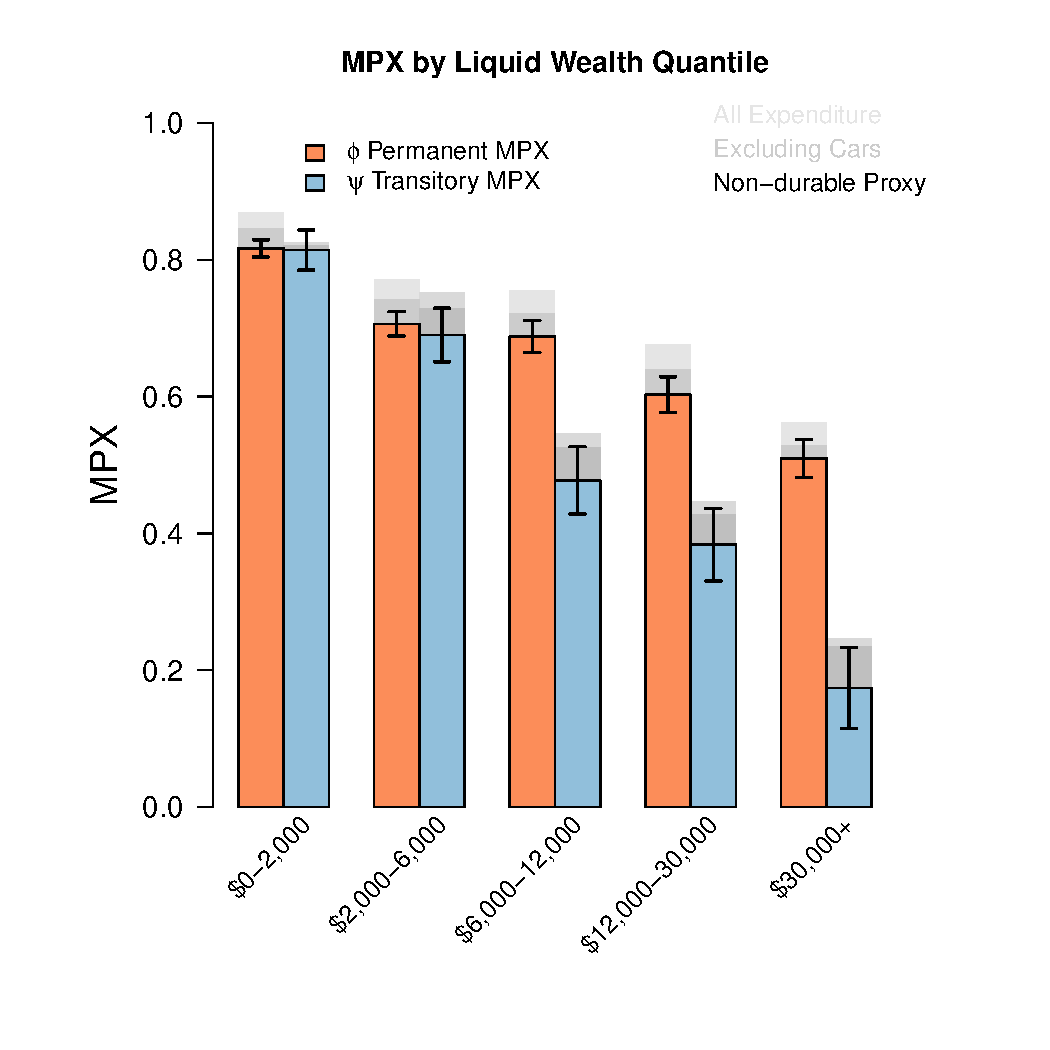
\includegraphics[scale=0.55]{\econtexRoot/Figures/MPXByDurables_nodurableproxy.pdf}
		\caption{MPX Removing Cars and Using the Nondurable Proxy Panel}
		\label{fig:MPXByDurables}
	\end{centering}
\end{figure}

In online appendix \ref{durables_appendix} we address this problem in two ways. First we show that our MPX estimates are unbiased in a simple model that includes durables, as long as we interpret the MPX out of transitory shocks to include durable expenditure (the correct definition for understanding aggregate demand) and the MPX out of permanent shocks to include only the consumption \textit{flow} from durables. Second, we are able to construct a nondurable consumption proxy for each household using registry data on car purchases. This proxy has very large measurement error, but will result in unbiased estimates of the MPC (excluding durables) to both permanent and transitory shocks. The estimated MPCs by liquid wealth quintile are shown in figure \ref{fig:MPXByDurables}. The figure shows the estimates using the nondurable proxy are, as expected, lower than those including all expenditures, although the change in magnitude is similar in size to the overall fraction of durable expenditure, suggesting durables do not play a special role in expenditures following transitory shocks. For the top quintile, durables do appear to play an outsized role, accounting for about a third of the expenditure response to transitory shocks.

%\FloatBarrier

\section{Conclusion}
In this paper we have presented a new method to measure the sensitivity of consumption to permanent and transitory income shocks for different groups of households. Our focus has been to use this method to test the microfoundations of heterogeneous agent models and quantify the importance of consumption heterogeneity for monetary policy. With administrative data from Denmark, we have been able to dig into the distribution of MPC across a variety of dimensions in far more detail than has previously been possible. We find that MPCs vary systematically and in ways that are important for monetary policy transmission, although the current generation of heterogeneous agent models struggle to fit the high sensitivity to income that we observe.

Our hope is that the method we present in this paper, or variants of it, can also be of use to economists in a variety of fields. More and more high-quality microdata on consumption are becoming available, such as the administrative data used here, or the even more detailed transaction-level data available from financial aggregators. If this trend continues, as we hope it will, methods such as ours will become even more valuable in bridging the gap between models and data.\\
%\begin{flushleft}
%\vspace{2cm}
%Edmund Crawley\\
%Federal Reserve Board\\
%Constitution Ave \& 20th Street NW, Washington, DC 20551, USA.\\
%edmund.s.crawley@frb.gov\\
%
%\vspace{1cm}
%Andreas Kuchler\\
%Danmarks Nationalbank\\
%Havnegade 5, 1093 Copenhagen K, Denmark.\\
%aku@nationalbanken.dk
%\end{flushleft}

\small
\bibliography{AllPapers}
\normalsize
%\processdelayedfloats

\pagebreak
\appendix
\renewcommand\thefigure{\thesection.\arabic{figure}}  
\renewcommand\thetable{\thesection.\arabic{table}}  

%\makeatletter
%\efloat@restorefloats
%\makeatother

\section*{Online Appendix}

\section{Identification with Time Aggregation}\label{sec:Identification}

\setcounter{figure}{0}   
\setcounter{table}{0} 
\input\econtexRoot/Appendices/Identification_levels.tex

\section{Sample Selection} \label{sample_selection}
\setcounter{figure}{0}   
\setcounter{table}{0} 
We choose to look at households whose head is between the ages of 30 and 55 in 2008, which is driven by the desire to remove households for which the assumption that most of the income growth is unexpected is not likely to be fulfilled. For the old and the young, individual households will likely have a lot of information about their income path that is not available to the econometrician (for example, the year in which they plan to retire, or the fact that they are on a specific career track with set expectations of promotion and pay raises). We also want to remove households whose income volatility is increasing or decreasing sharply. Figures \ref{fig:VarianceByAge} and \ref{fig:MPXByAge} show how our estimates of both income variance and MPX vary with age. The dots represent the point estimate for each age, while the lines are the centered moving averages over the five nearest age groups. The solid black line shows the total variance of income growth over one year. It should not be surprising that income growth for households with heads in their 20's is highly volatile. This volatility plateaus around the age of 35 and stays at a constant level until retirement, at which point it temporarily grows before falling to an even lower level. We can see that while both transitory and permanent shocks to income are high early in life, permanent income shocks are particularly high while individuals find their place in the workforce. From the ages of 30 to 55, both transitory and permanent shocks are approximately the same size and remarkably stable. At retirement, shocks to permanent income rise---not surprising, as the model sees retirement itself as a shock---even as transitory income variance declines.

As the model assumes the variance to permanent and transitory shocks to be constant in the observed period, interpretation of the numbers outside of the 30 to55 age group needs to be treated with care. However, the figure clearly shows that within this age group the assumption of constant variance appears to be a reasonable one.

The dotted black line shows the variance of $\Delta y$, assuming no persistence in the transitory component. The fact that this line is slightly above the empirical variance of $\Delta y$ is consistent with some persistence in the transitory component of income, justifying our decision to exclude growth over one and two years in our identification.

The level of both permanent and transitory shock variance for households aged 30 to 55 is approximately 0.0035, reflecting a standard deviation of 6\%. Estimates using U.S. data are significantly higher, especially for the transitory shock variance (for example, \cite{carroll_nature_1997} estimate 0.02 for permanent and 0.04 for transitory). This difference may be due to lower income inequality in Denmark, more progressive taxation, and more generous unemployment insurance. The lower transitory variance will also be due to significantly reduced measurement error relative to the survey-based U.S. data. 
\begin{figure} 
	\begin{centering}
		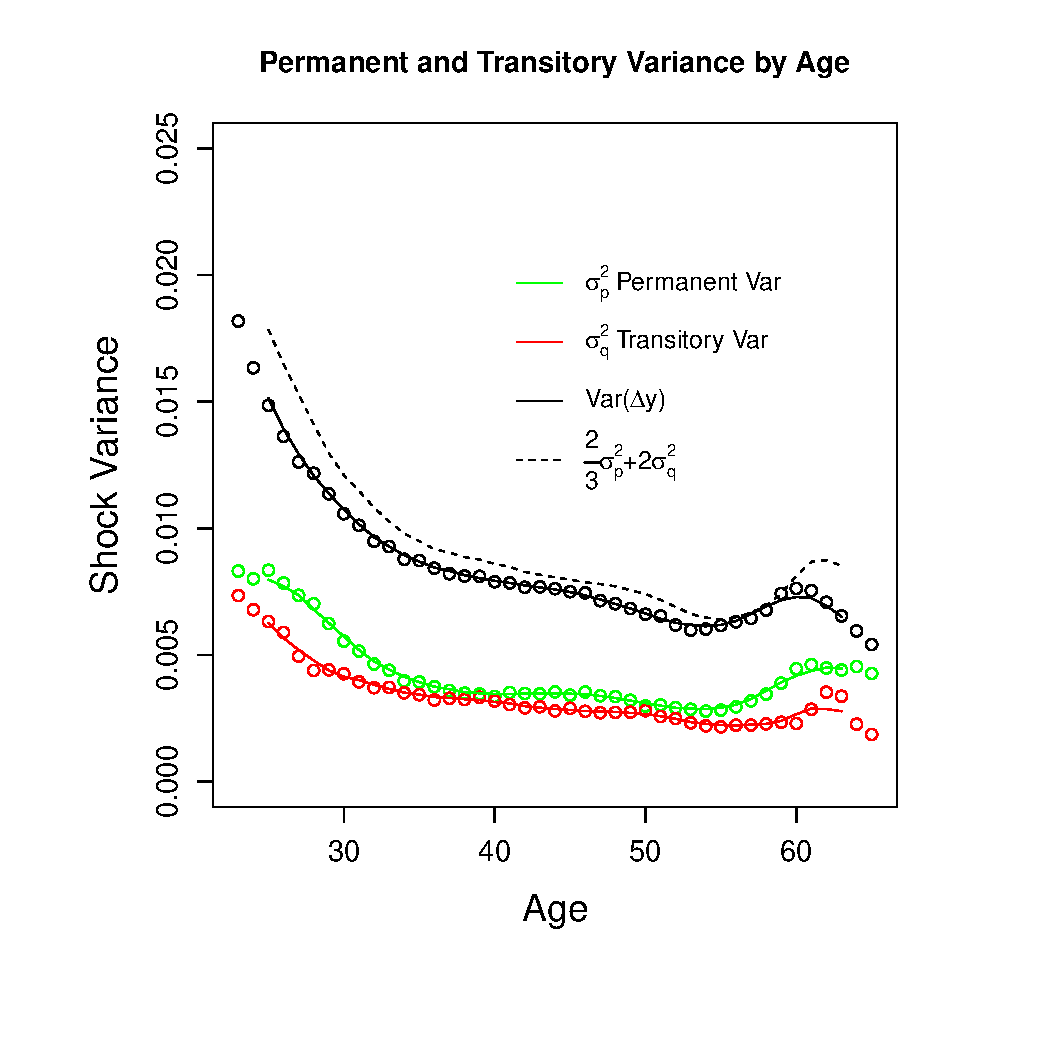
\includegraphics[scale=0.6]{\econtexRoot/Figures/VarianceByAge_level_lincome_head.pdf} 
		\caption{Permanent and Transitory Shock Variance by Age}
		\label{fig:VarianceByAge}
	\end{centering}
\end{figure}
\begin{figure} 
	\begin{centering}
		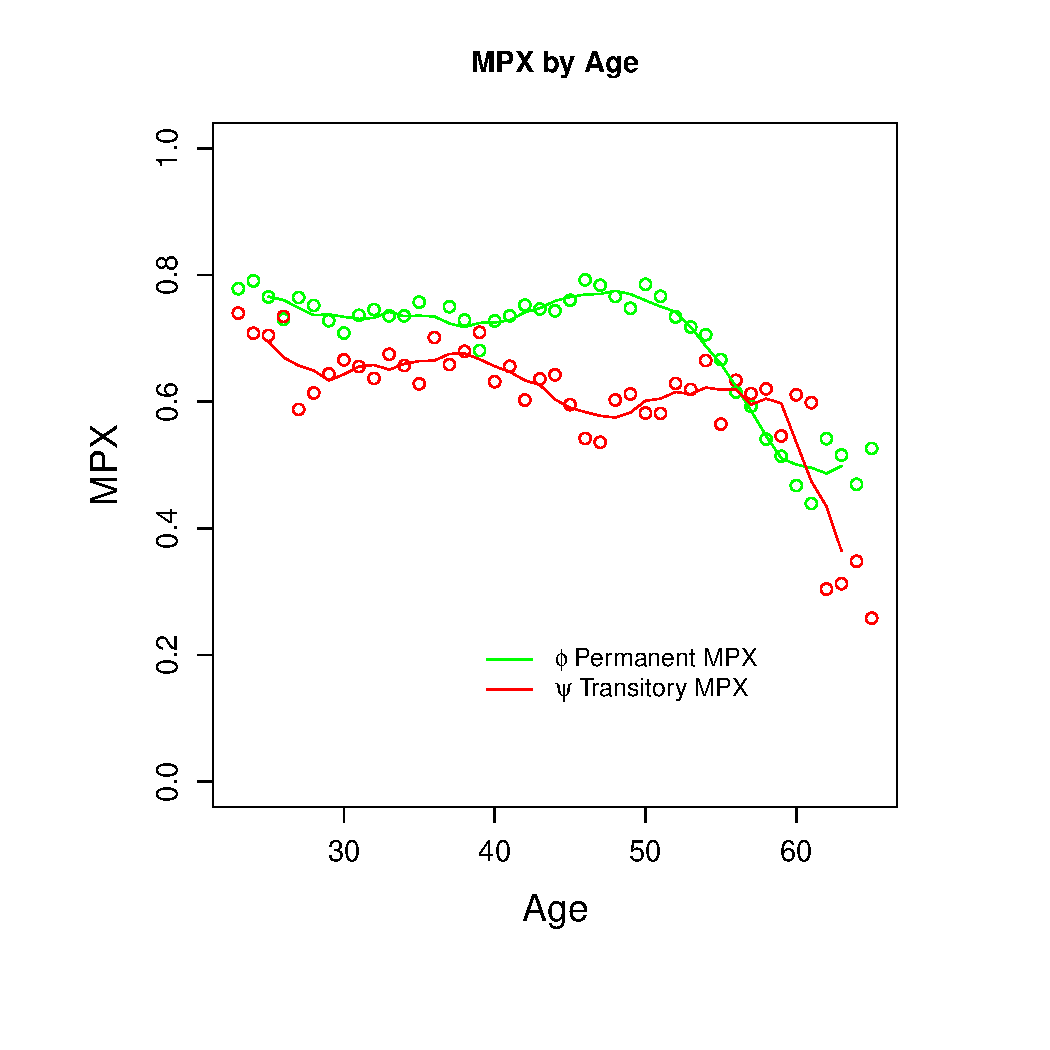
\includegraphics[scale=0.6]{\econtexRoot/Figures/MPXByAge_level_lincome_head.pdf} 
		\caption{MPX by Age}
		\label{fig:MPXByAge}
	\end{centering}
\end{figure}

\section{The Danish Mortgage Market} \label{mortgage_market}
\setcounter{figure}{0}   
\setcounter{table}{0} 
Mortgage loans in Denmark are issued by specialized mortgage banks, which fully finance loans by issuing bonds. Interest rates are directly determined by sales prices at the bond market. That is, borrowers only pay the bond market interest rate plus a supplementary fee for the mortgage bank. 
Most loans are issued as 20- or 30-year loans, and households can only obtain loans from mortgage banks for up to 80\% of the value at loan origination of properties used as permanent residences. The remaining (more insecure) part of the funding may be provided by commercial banks. The close link between loans and bonds, as well as fixed loan-to-value ratios, fast foreclosure procedures, full recourse, etc., mean that mortgage banks do not assume significant market risks. The status of Danish covered mortgage bonds as a safe asset class (AAA-rated by, e.g., S\&P) implies that borrowers have access to very cheap real estate funding.

\begin{figure} 
	\begin{centering}
		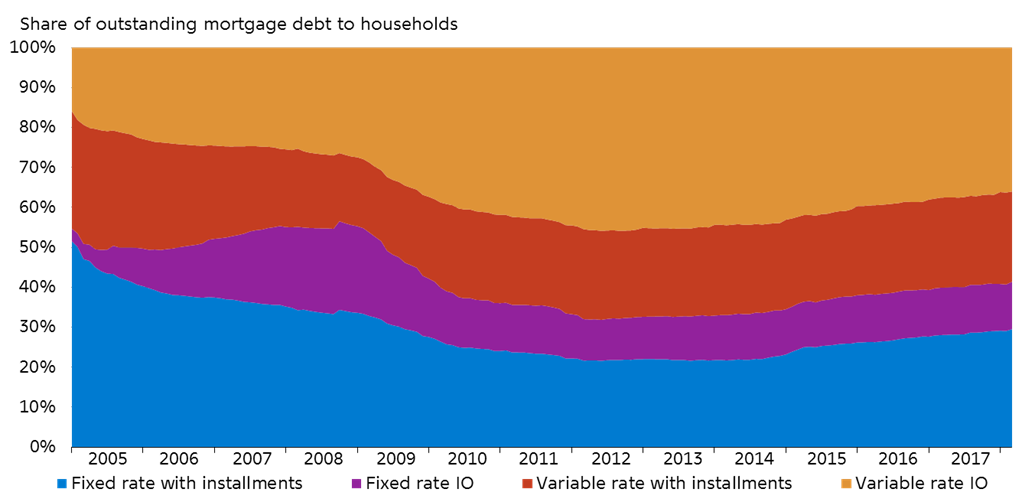
\includegraphics[scale=0.7]{\econtexRoot/Figures/mortgage_by_type.png} 
		\caption{Mortgage Debt by Type (All Households)
		{\\ \emph{\footnotesize
	{Source: Danmarks Nationalbank}}
	}}
		\label{fig:mortgage_by_type}
	\end{centering}
\end{figure}

The Danish mortgage system has been functioning for two centuries, but significant liberalization has taken place over the past 20 years. Variable interest loans were (re-)introduced in 1996, while interest only loans were introduced in 2003. These new loan characteristics are by now very popular; see figure \ref{fig:mortgage_by_type}. In contrast to the United States, where most mortgage debt is fixed rate, 40\% of mortgage debt in Denmark is variable rate, with interest fixation periods mostly between six months and five years. Fixed-rate loans come with an option for early redemption, which implies that in practice, refinancing of fixed-rate mortgages often takes place, both when interest rates decrease and increase. The latter may be attractive because borrowers have the option to repay their loan by purchasing the corresponding amount of bonds. When interest rates increase, the bond value decreases, so the option to repay the loan by purchasing the corresponding amount of bonds in essence acts as an equity insurance.  

\begin{figure} 
	\begin{centering}
		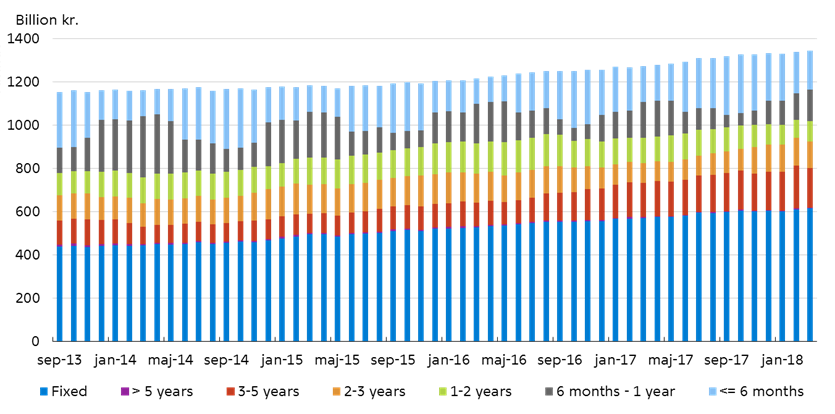
\includegraphics[scale=0.7]{\econtexRoot/Figures/mortgage_by_maturity.png} 
		\caption{Mortgage Debt by Maturity (All Households Excluding Self-employed)
		{\\ \emph{\footnotesize
	{Source: Danmarks Nationalbank}}
	}}
		\label{fig:mortgage_by_maturity}
	\end{centering}
\end{figure}

Around one-fourth of the total loan balance is due to have interest rates reset over a 12-month period (see figure \ref{fig:mortgage_by_maturity}). This figure only comprises loans that automatically will have a new interest rate and not active decisions to refinance or extract equity. 

\section{Details on the Calculation of NNP and URE}
\setcounter{figure}{0}   
\setcounter{table}{0} 
\label{URE_NNP_appendix}
The Net Nominal Position (NNP) and Unhedged Interest Rate Exposure (URE) for the various sectors in the Danish economy are calculated from our household-level dataset as well as the financial accounts from the national accounts statistics. All calculations are based on average values over the years 2009 to 2015, deflated by the consumer price index. 

\subsection{NNP and URE for Households}
The NNP for households is calculated as financial assets minus liabilities. As financial assets, we include bank deposits as well as the market value of securities (excluding shares). Liabilities include all debt to financial institutions (including credit card debt) as well as publicly administered student debt, tax debt and other debt to government bodies. These data are reported to the tax authorities by financial institutions on behalf of the households. 

URE is calculated as annual savings (i.e. after-tax income minus expenditure) plus maturing assets minus maturing liabilities. As maturing assets, we include all bank deposits, thereby assuming that they are floating rate. We assume a maturity of five years for securities held by households and therefore include 20\% of the value of securities. Regarding liabilities, we assume that all bank debt is floating rate. According to the interest rate statistics collected by Danmarks Nationalbank since 2013, on average 95\% of bank debt from households is floating rate, most of which is tied either to a market reference rate or to the Danmarks Nationalbank rate on certificates of deposit, with immediate adjustment. For mortgage debt, we have detailed information allowing us to calculate the stock of debt which is due to have interest rates reset over the coming 12 months. Voluntary refinancing of mortgage loans, with or without extraction of additional equity, takes place to a large extent in Denmark. Our measure of maturing liabilities only includes the loans that are contractually due to have their interest rates reset, and we do not attempt to estimate the amount of additional refinancing. For remaining liabilities, which constitute very small amounts, we have no information regarding maturity, so we assume five years. 

\subsection{Other Sectors}
NNP for the other sectors in the economy is obtained from the financial accounts statistics compiled by Danmarks Nationalbank. To most closely resemble the definition used in the household-level data, we define NNP as net assets (i.e., assets minus liabilities) in the following categories: "Currency and deposits", "Securities other than shares", "Loans", and "Trade credits and other accounts receivable/payable". 

NNP for the whole economy should, in principle, sum to 0. However, the household-level microdata on bank deposits that we have access to is exclusive of certain types of savings (specialized children's savings accounts as well as some forms of pension savings accounts administered by banks), which are included in the financial accounts statistics. For the age group included in our sample, these types of accounts can be assumed to be largely illiquid. We therefore group those deposits (33 billion USD) together with the assets of pension funds (see table \ref{table:aggElas}).\footnote{In practice, this amount is calculated as a residual, which may also reflect other minor differences between the household-level data and the national accounts statistics. For example, holdings of banknotes and coins are not observed in the microdata but are allocated based on certain assumptions in the financial accounts. For our exercise, the impact of such other differences is likely to be very small.}

URE for non-households is also based on the financial accounts. In the national accounts, we do not observe the maturity of different asset and liability classes. We hold household URE fixed at the values from the micro-level data and take advantage of the identity that total URE in the economy must be 0 to calibrate the maturity for the remaining sectors of the economy. This results in a maturity of assets and liabilities for non-households of 3.65 years.

\section{Comparison to \cite{blundell_consumption_2008}} \label{BPP_compare}
Are the differences in our estimates to those in BPP driven by the data or by the method? Here we apply BPP's original method to moments obtained from the Danish administrative data. Applied to the entire dataset, this method estimates the response to permanent income shocks to be 0.81 and to transitory income shocks to be 0.12. The response to permanent income shocks is in line with our method, while the response to transitory income shocks is significantly biased towards zero, although still larger than that obtained using PSID data.

\begin{figure} 
	\begin{centering}
		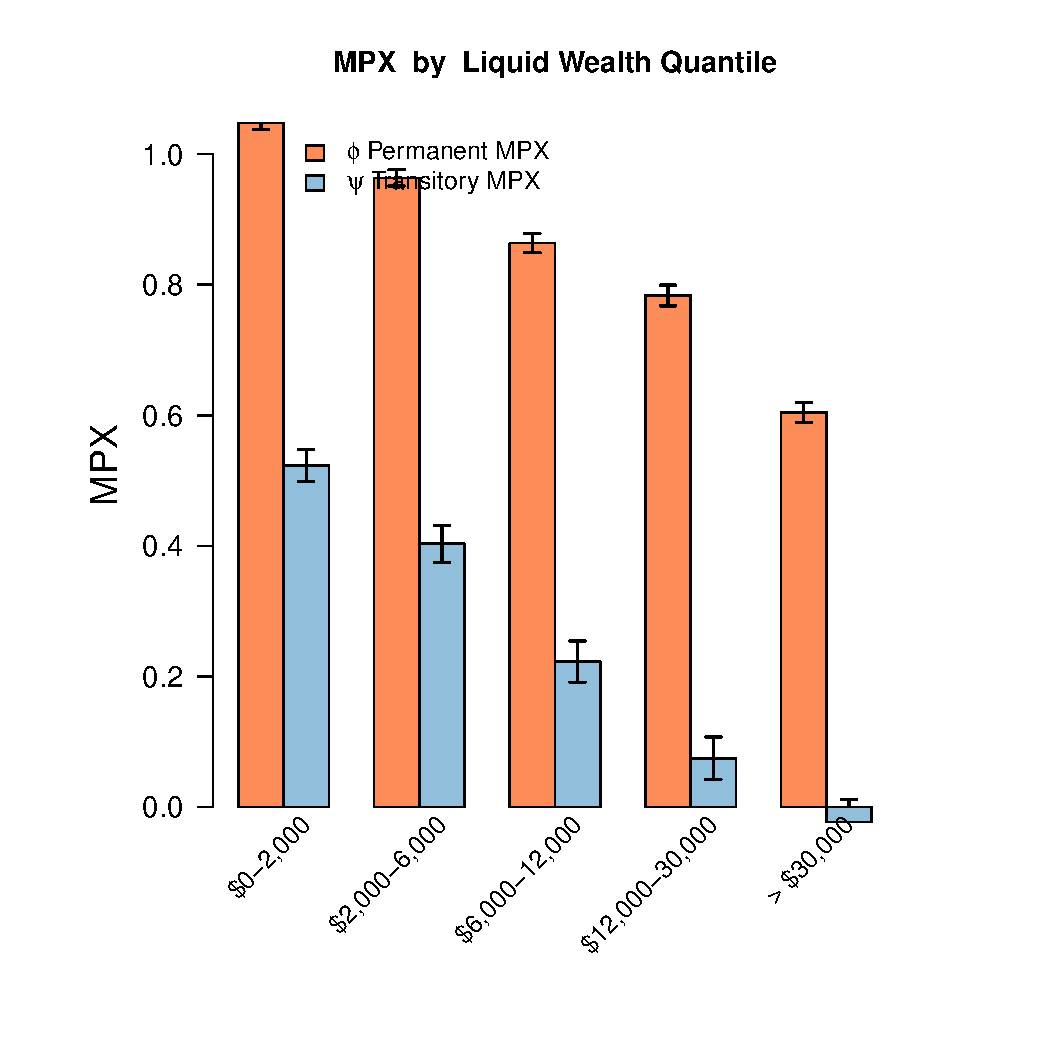
\includegraphics[scale=0.4]{\econtexRoot/Figures/MPXByLiquidWealthBPP_level_lincome_head.pdf}
		\caption{Estimates by Liquid Wealth Quintile Obtained Using BPP's Methodology}
		\label{fig:BPP_liquid}
	\end{centering}
\end{figure}

Figure \ref{fig:BPP_liquid} shows the results of using BPP's method on quintiles of liquid wealth. While the downward sloping pattern is evident, the magnitudes are very different to those from our method shown in figure \ref{fig:MPXByLiquidWealth} in the paper.  

Our method differs from BPP in two respects: first we model time aggregation and second we impose that consumption responses to transitory income shocks are short lived, in contrast to the random walk behavior in BPP. \cite{crawley_time_2019} shows how just the first of these, modeling time aggregation, significantly changes BPP's estimates in the PSID data. With the high MPX's that we estimate in our data, it is clear that the random walk assumption cannot be valid. If we only make this first change and estimate again using the Danish administrative data, we estimate the response to permanent income shocks to be 1.18 and to transitory income shocks to be 1.50. These unreasonably high estimates come as a result of the assumption that consumption follows a random walk. In particular, the fact that the response to transitory income shocks is significantly greater than one comes from the method extending the short term response over the period of one year.

This exercise has shown that the original BPP method is both biased and sensitive to assumptions made about the path of consumption. In appendices \ref{Consumption_persistence}, \ref{rip_hip_appendix}, and \ref{time_varying_risk} we show that, in contrast, our method is relatively robust to misspecification.

\section{Persistent Consumption Response} \label{Consumption_persistence}
\setcounter{figure}{0}   
\setcounter{table}{0} 

Our estimation procedure makes the assumption that the consumption response to a transitory income shock decays to zero in a period of two years or less. A slower decay will lead to a downward bias in our estimates of the transitory MPX. Figure \ref{fig:DecayBias} shows the results of our estimation procedure on simulated data under two different assumptions about the transitory consumption response.

The exponential decay line assumes that the consumption flow following a transitory shock decays exponentially.\footnote{Standard buffer-stock models give rise to a consumption response that decays very close to exponentially.} We vary the decay rate to match a range of year 1 MPCs and assume that the entire transitory income is eventually consumed. For high MPCs, and especially those over 0.5, there is very little bias. However, for MPCs significantly below 0.5 our method results in downward-biased estimates. This bias arises because low MPCs, combined with exponential consumption decay, result in a relatively stable consumption flow over the first few years that has not declined close to zero after two years.

Empirical evidence suggests that in fact the consumption response to a transitory shock decays quickly in the first few months and then more slowly after that.\footnote{Both \cite{fagereng_mpc_2016} and \cite{gelman_what_2016} provide evidence for this.} The ``Fagereng et al.'' line in figure \ref{fig:DecayBias} shows the MPC estimate in simulated data in which the consumption response decays according to the estimates made in \cite{fagereng_mpc_2016}. In this case, the fast decay in the first few months results in a smaller bias than the exponential case for low MPCs, while the fact that the decay is slower following these first months results in a larger bias for high MPCs. Overall it seems likely that our assumption about the persistence of the consumption response leads to a slight downward bias across the range of MPCs.

We also show that our MPX estimates are not very sensitive to the choice of $N$ (years of growth in our identification equations) between 3 and 6, which lends further support to the fact that assuming a two-year limit does not bias our results too much.\footnote{Using $N$ equal to 4 and 5 instead of 3, 4, and 5 allows us to extend the consumption response out to three years, at the expense of losing data and becoming more sensitive to misspecification of the income process.}
\begin{figure} 
	\begin{centering}
		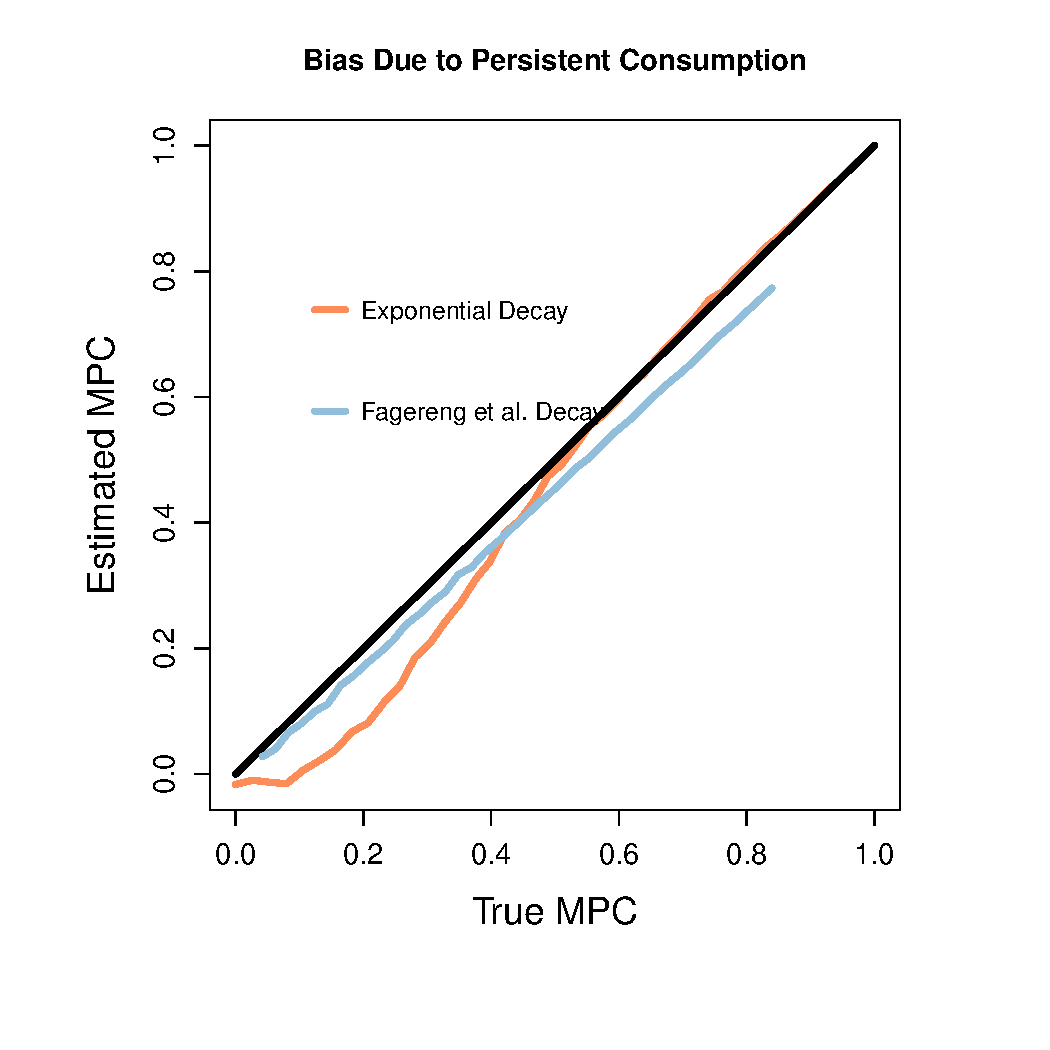
\includegraphics[scale=0.4]{\econtexRoot/Figures/DecayBias.pdf}
		\caption{Bias from Persistent Consumption}
		\label{fig:DecayBias}
	\end{centering}
\end{figure}

\subsection{Details on Section \ref{Consumption_persistence} Simulations}
For the simulations in section \ref{Consumption_persistence} we divided each year into 20 sub-intervals. Both permanent and transitory shocks occur each period, and the transitory shocks have no persistence. At an annual frequency the variance of permanent and transitory shocks are equal. Households spend their permanent income each period, along with their consumption response to the history of transitory shocks. For the exponential decay model, this is
\begin{align*}
c_t = p_t + (1-\rho)\sum_{n=0}^{\infty}\rho^n \varepsilon_{t-n}
\end{align*}
In \cite{fagereng_mpc_2016} the T year MPC is estimated as a function:
\begin{align*}
\text{MPC}_T = \theta_1 T^{\theta_2}
\end{align*}
where $\theta_1$ controls the size of the response and $\theta_2$ the speed of decay. We vary $\theta_1$ and choose $\theta_2= 0.2142$ according to their estimate. In this model consumption in period $t$ (measured in sub-intervals) is:
\begin{align*}
c_t = p_t + \theta_1\sum_{n=0}^{\infty}\Big( (\frac{n+1}{20})^{\theta_2} -(\frac{n}{20})^{\theta_2} \Big)\varepsilon_{t-n}
\end{align*}
We then time aggregate both income and consumption over each 20-sub-interval period, choose a sample of 13 years, and run our estimation procedure with $N=3,4,5$. The transitory MPC estimates are shown in figure \ref{fig:DecayBias}, and the permanent estimates are shown in figure \ref{fig:DecayBias_phi}. The bias in permanent estimates is small across the range of transitory MPCs.
\begin{figure} 
	\begin{centering}
		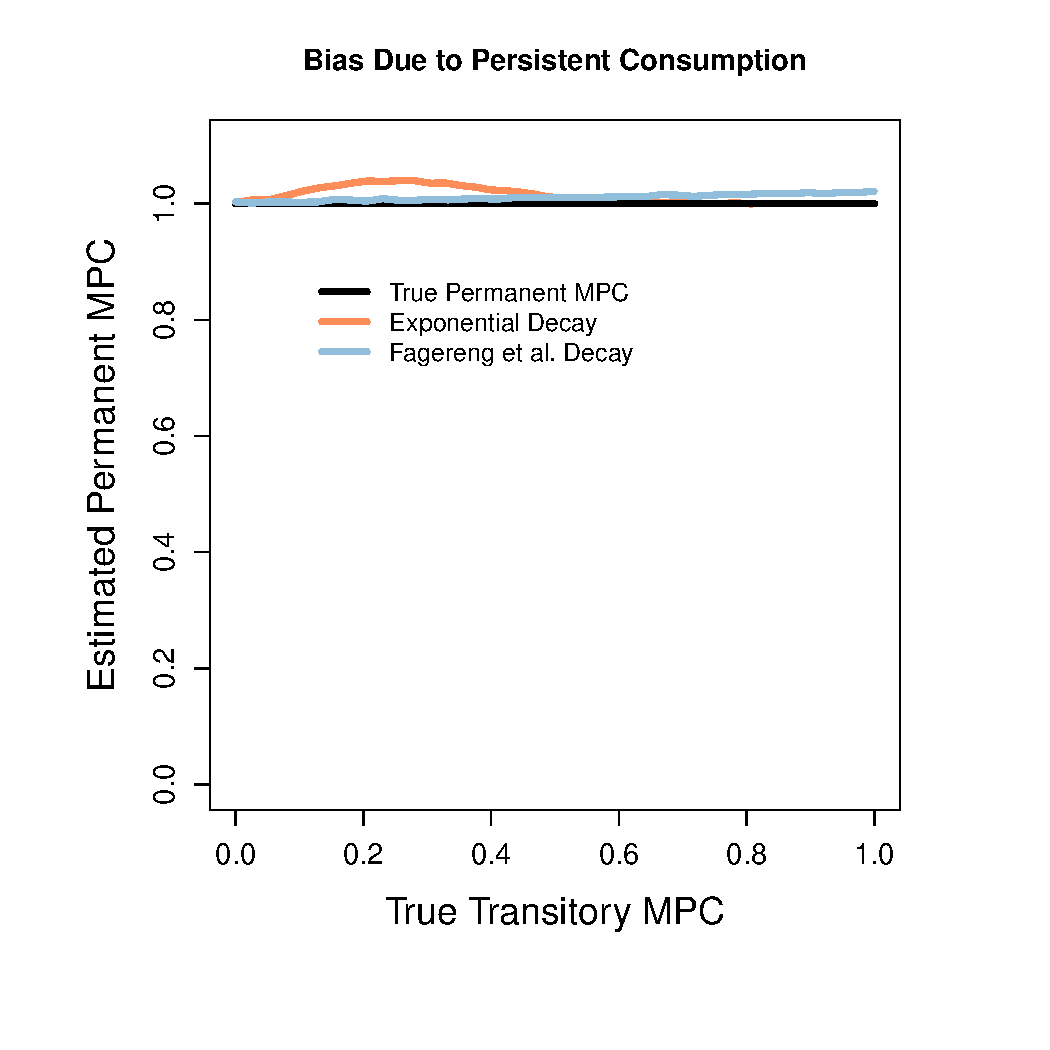
\includegraphics[scale=0.4]{\econtexRoot/Figures/DecayBias_phi.pdf}
		\caption{Bias from Persistent Consumption}
		\label{fig:DecayBias_phi}
	\end{centering}
\end{figure}
\subsection{Estimates Using Different Values of $N$}
\begin{center}
	\captionof{table}{$\psi$ Estimates Using Different $N$}
	\label{table:psi_estimates}
	\input ./Tables/Psi_array_empirical.tex
\end{center}
Table \ref{table:psi_estimates} shows the estimates of the transitory MPX that we recover from our estimation sample when we just use $N=n_1,n_2$ in our identification equations \ref{variance} and \ref{covariance}. Remember in our main results we used GMM with $N=3,4,5$ and we have circled $N=3,5$ to highlight where we get identification from in the paper. The purpose of this exercise is to show that the estimation results are not very sensitive to the values of $N$ chosen, providing more evidence that the assumption we made that the transitory consumption response lasts less than two years is not biasing our results significantly. In fact, the results are not changed dramatically even when $N=1,2$, which suggests the majority of the transitory consumption response is very short-lived.


\begin{comment}
\section{Benchmark Model and Taste Shock Extension} \label{model}
In this section we calibrate a standard incomplete markets model to Danish characteristics, including the liquid wealth distribution in Denmark, and use it to see if we can match the consumption responses we measure in the data.\footnote{By calibrating to the liquid wealth distribution, we are implicitly assuming that households cannot access any of their illiquid wealth, similar to the two asset model in \cite{auclert_ikc}. A model such as \cite{violante_wealthy_2014} or \cite{gorea_liquidity_2017} that allows households to buy and sell an illiquid asset at a cost would result in lower overall MPCs.}

Motivated by the fact that the standard model results in lower transitory MPX numbers than we find in the data, we make a simple extension to the model to account for potentially large preference shocks. We propose that such shocks, which have generally played a much smaller role in the literature than income shocks, are perhaps quantitatively more important for precautionary savings behavior.

\subsection{Benchmark Model Calibrated to Danish Data} \label{benchmark_model}
Our baseline model is the now very familiar buffer-stock saving model of \cite{carroll_buffer_1997}. Given market resources ($\boldmath{\mLevBF}_t$), households in this model maximize expected utility
\begin{align*}
\mathbb{E}_t \sum_{s=t}^{\infty} \beta^s u(\cLevBF_s)
\end{align*}
subject to the constraints\footnote{Here $\cLevBF_t$ is consumption, $\aLevBF_t$ end-of-period assets, $R$ the constant real interest rate (set to 1.065), $\bLevBF_t$ beginning-of-period assets, $\yLevBF_t$ income, and $\pLevBF_t$ permanent income.}
\begin{align*}
\aLevBF_t = \mLevBF_t - \cLevBF_t \\
\bLevBF_t = R\aLevBF_t \\
\yLevBF_t = \theta_t \pLevBF_t \\
\pLevBF_t = \Psi_t \pLevBF_{t-1} \\
\mLevBF_t = \bLevBF_t + \yLevBF_t
\end{align*}
where the felicity function, $u(\cLevBF)$, is CRRA. We calibrate our model to match both the income uncertainty (as measured using our methodology) and the liquid wealth distribution in Denmark. The model is quarterly, and we aggregate both income and consumption to the annual frequency where required.

Permanent income, $\pLevBF_t$, experiences normally distributed shocks, $\Psi_t$, with (annualized) variance equal to 0.004, matching our population estimate. Transitory income shocks, $\theta_t$, are normally distributed with (annualized) variance 0.0035 if employed, and a small 0.001 probability of a zero income, unemployed, state that induces a natural borrowing constraint at zero.

We examine an economy in steady state, where each agent has a probability $1/160$ of dying each quarter and being replaced by another agent with permanent income equal to one, and no initial wealth.

To be able to match the liquid wealth distribution, especially at the low end, we follow \cite{krusell_income_1998} and \cite{carroll_distribution_2017} and allow for ex-ante heterogeneity in the discount factor $\beta$. Specifically, an agent $i$ has a discount factor $\beta_i$ where $\beta_i$ is i.i.d. across agents and follows a uniform distribution between $\beta_{low}$ and $\beta_{high}$. These two parameters allow us to match the fact that while the mean level of liquid assets is high, about half of all households have close to zero liquid assets. Matching the lower part of this distribution is critical to generate transitory consumption elasticities substantially above zero. The Lorenz curve for liquid assets, both in the data and in the model, is shown in figure \ref{fig:Lorenz}.\footnote{We calibrate to the 20th, 40th, and 60th percentile of liquid wealth, leaving out the 80th percentile, to better match the wealth of the lower half of the distribution, which is necessary to achieve reasonably high MPCs in a model like this. The figure shows that the fit in the upper half of the distribution is less precise. Our estimates of $\beta_{low}$ and $\beta_{high}$ are 0.978 and 0.992, respectively.}
\begin{figure} 
	\centering
	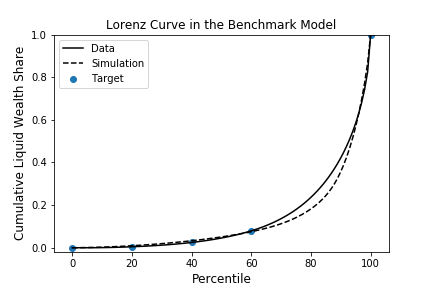
\includegraphics[scale=0.45]{\econtexRoot/Figures/benchmark_Lorenz.png}
	\caption{Lorenz Curve for Danish Liquid Assets}
	\label{fig:Lorenz}
\end{figure}

\subsection{Model with Preference Shocks}
The baseline model exhibits two features in tension with the data. First, the marginal propensity to consume out of transitory income shocks, while exhibiting the right shape relative to liquid wealth, is too low relative to the data. Second, as would be expected in such a consumption-smoothing model, the path of expenditure is significantly less volatile than income. However, the data show the opposite: the standard deviation of changes in expenditure is around 0.37, compared to 0.12 for income. There is very little evidence on the true size of expenditure shocks, partly because of large measurement errors known to be present in consumption survey data. While we believe the 0.37 number from our data also contains measurement error, as well as large expected expenditures such as new cars for which finance may be readily available, it seems likely that the expenditure shocks could be large. Indeed, typical financial advice to maintain a buffer stock will mention unexpected costs such as medical bills or a leaky roof before income shocks.\footnote{For example, in 2016,  Forbes Magazine suggested ``you could find yourself thrown off by a chipped tooth or fender bender. So having an emergency fund padded with nine months of the highest earner's net income may help give you a bit more peace of mind that you could weather a financial storm.''} A simple tweak to the baseline model can help the model fit the data along both these dimensions. To achieve this we add a preference shock to expected utility:
\begin{align*}
\mathbb{E}_t \sum_{i=t}^{\infty} \beta^i \mathcal{X}_i u(\cLevBF_i)
\end{align*}
where $\mathcal{X}_i$ is i.i.d. and calibrated such that the variance of consumption is large.\footnote{We choose preference shocks with an annual standard deviation of 0.3. While this seems large, the resulting consumption change standard deviation is 0.18, significantly lower than 0.37 that we observe in the data.}

\subsection{MPX by Liquid Wealth} 
The top panel of figure \ref{fig:CSTW} shows how the transitory MPX of the two models compares with the data. While the fact that the MPX decreases with the liquid wealth quintile is robust in both models and in the data, there are two features worth noting. 

First, large preference shocks are required to push the transitory MPX close to the levels we see in the data. Many recent papers, such as \cite{krueger_macroeconomics_2016}, have attempted to carefully quantify the macroeconomic dynamic consequences of a serious heterogeneous agent model but thus far have not included significant preference shocks in their calibrations. The evidence here suggests that such shocks may have a quantitatively important role to play, especially in increasing the MPC. To the extent that the precautionary motive is driven by preference shocks as opposed to income shocks, social insurance for unemployment will not reduce precautionary savings as much as these models presently suggest.

Second, neither of the two models is able to explain the high MPX out of transitory shocks that we observe for the top quintile of liquid assets. These households, which hold a mean balance above \$30,000, appear very responsive to transitory shocks despite the large buffer stock they could potentially use to smooth income shocks.
\begin{figure} 
	\begin{centering}
		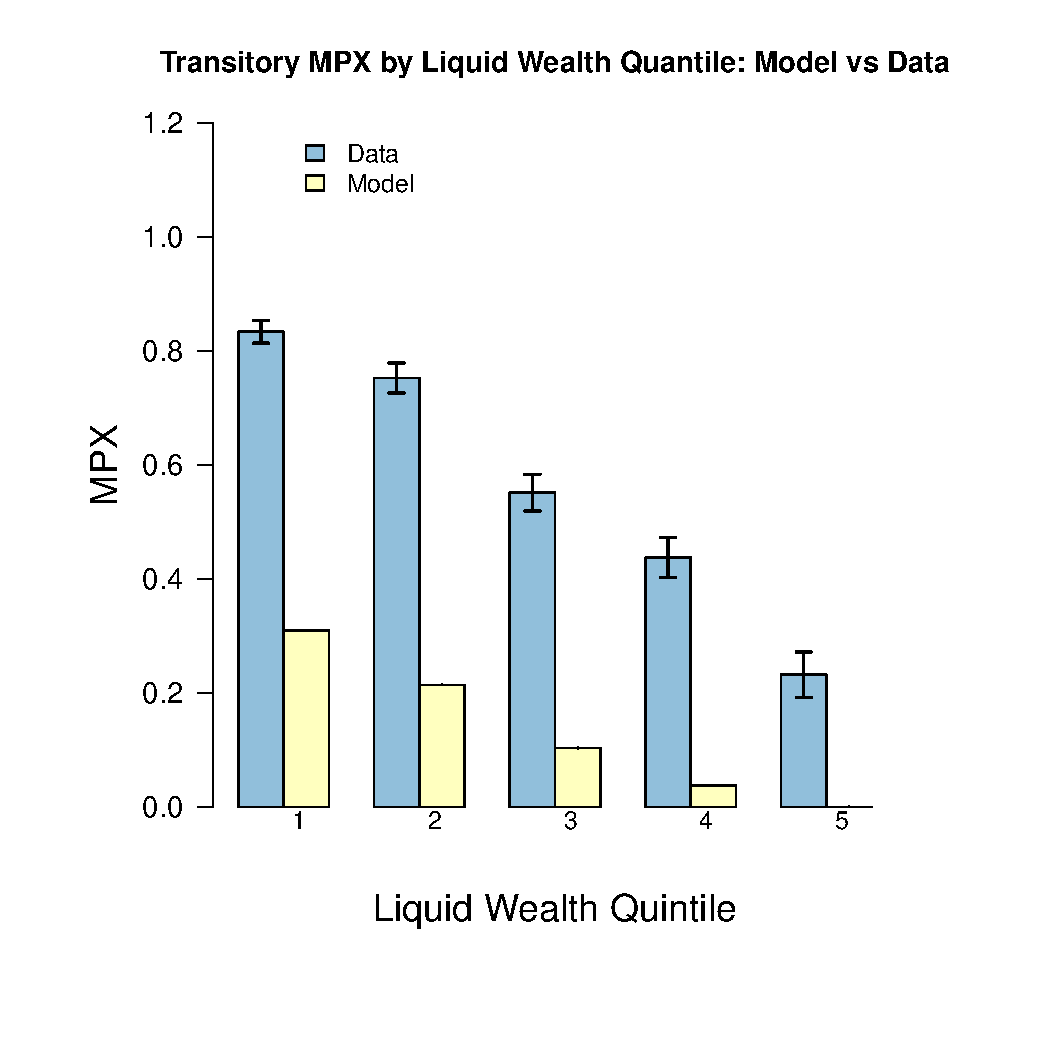
\includegraphics[scale=0.4]{\econtexRoot/Figures/CSTW_tran_denmark.pdf}
		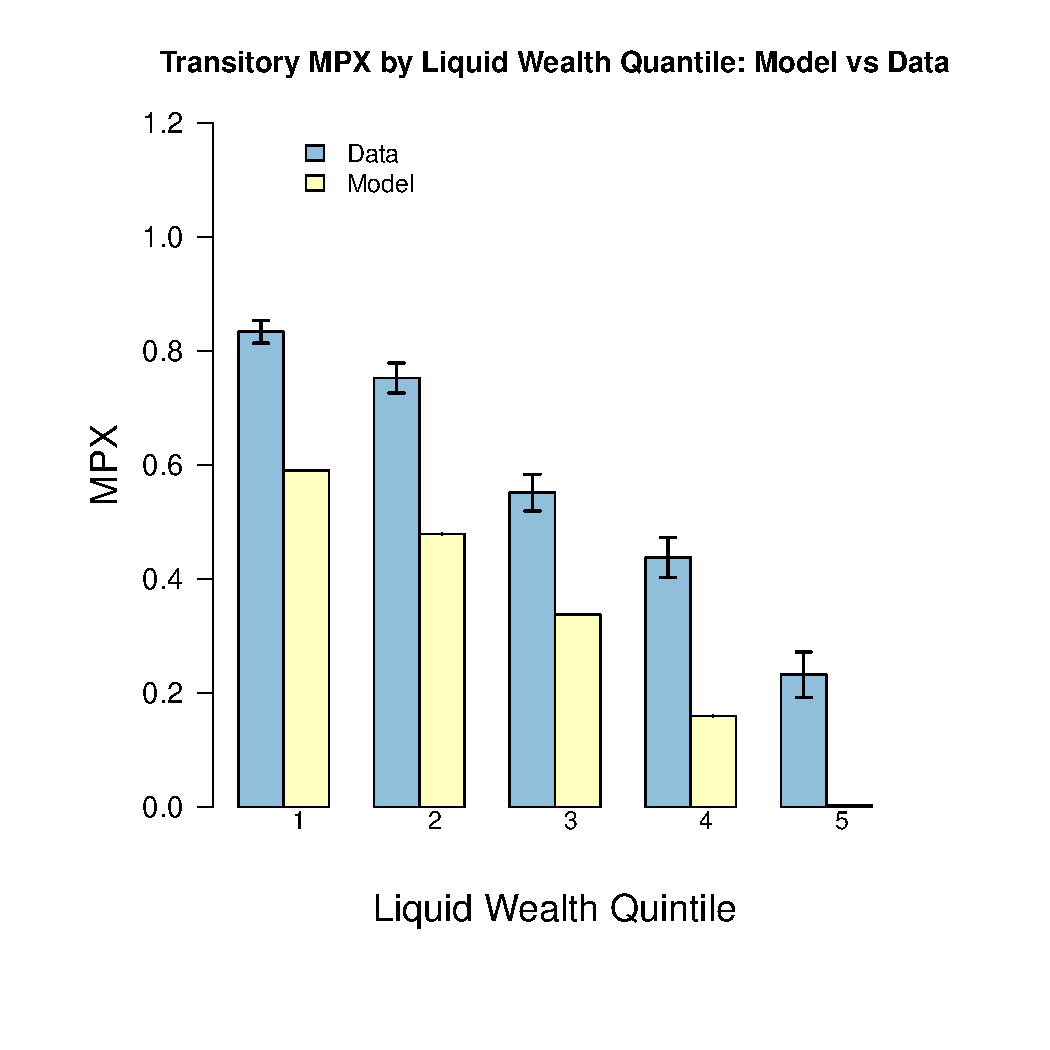
\includegraphics[scale=0.4]{\econtexRoot/Figures/CSTW_tran_denmark_pref.pdf}
		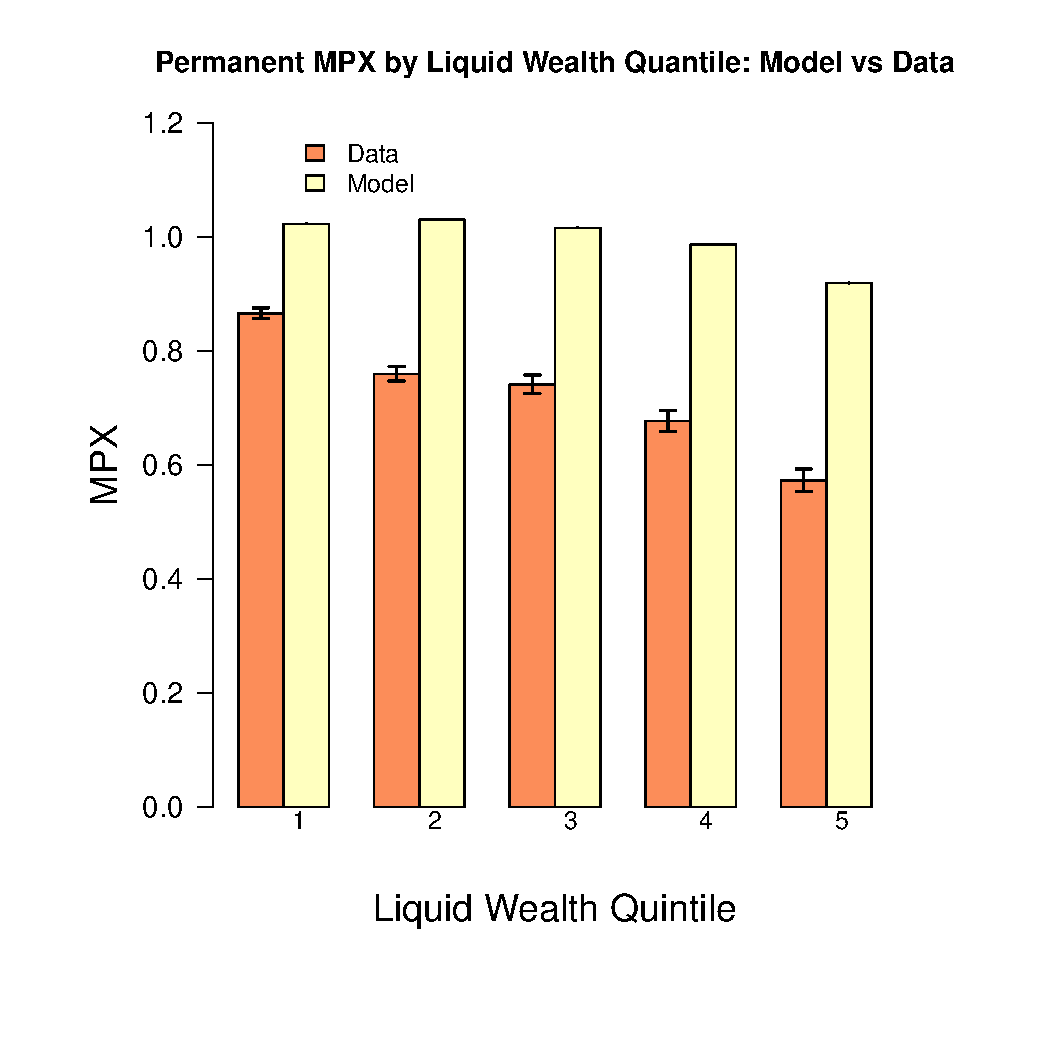
\includegraphics[scale=0.4]{\econtexRoot/Figures/CSTW_perm_denmark.pdf}
		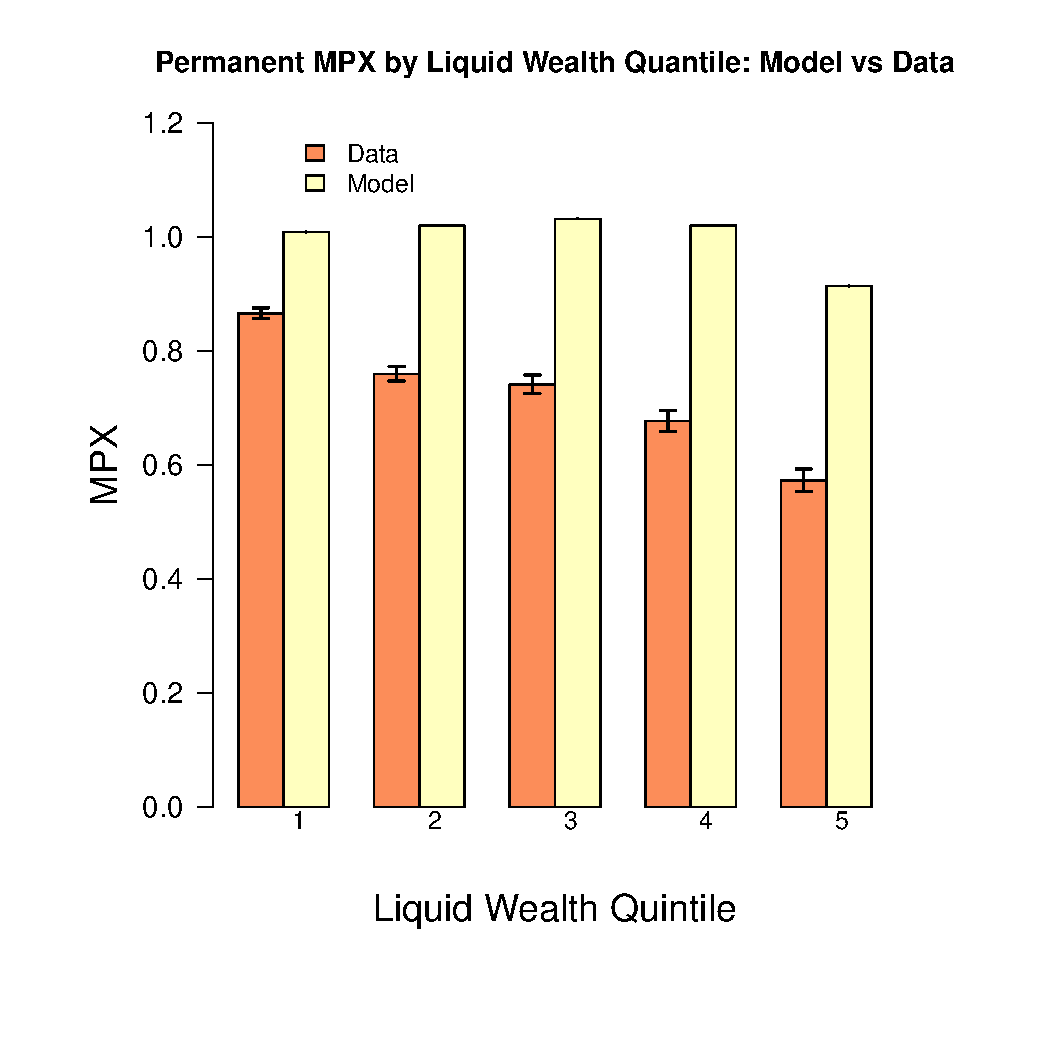
\includegraphics[scale=0.4]{\econtexRoot/Figures/CSTW_perm_denmark_pref.pdf}
		\caption{Baseline model (LHS) and Preference Shock Model (RHS) with the Data}
		\label{fig:CSTW}
	\end{centering}
\end{figure}

The bottom panel of figure \ref{fig:CSTW} shows another failure of both of these two simple models: neither is able to capture the fact that the consumption response to permanent shocks is substantially below 1, even for middle and low quintiles of liquid wealth. \cite{straub_consumption_2018} shows that a lifecycle model with nonhomothetic preferences may do better along this front.

\subsection{Persistent Consumption in the Preference Shock Model}
Using a model we are able to calculate precisely the partial derivative of expenditure with respect to transitory income. To be comparable to the time period of our empirical MPX we take the mean MPX over one, two, three and four quarters:\footnote{Remember our empirical method measures the covariance of income with expenditure in the same calendar year. If the shock happens in the first quarter, then we will count expenditure over the next four quarters. If the shocks happen in the final quarter, then only one quarter of expenditure will be captured.}
\begin{align*}
\text{MPX}_{\text{model}} = 1 - \frac{1}{4}\sum_{i=1}^{4}(1-\text{MPX}_q)^i 
\end{align*}
where $\text{MPX}_q$ is the partial derivative in the quarterly model.
\begin{figure} 
	\begin{centering}
		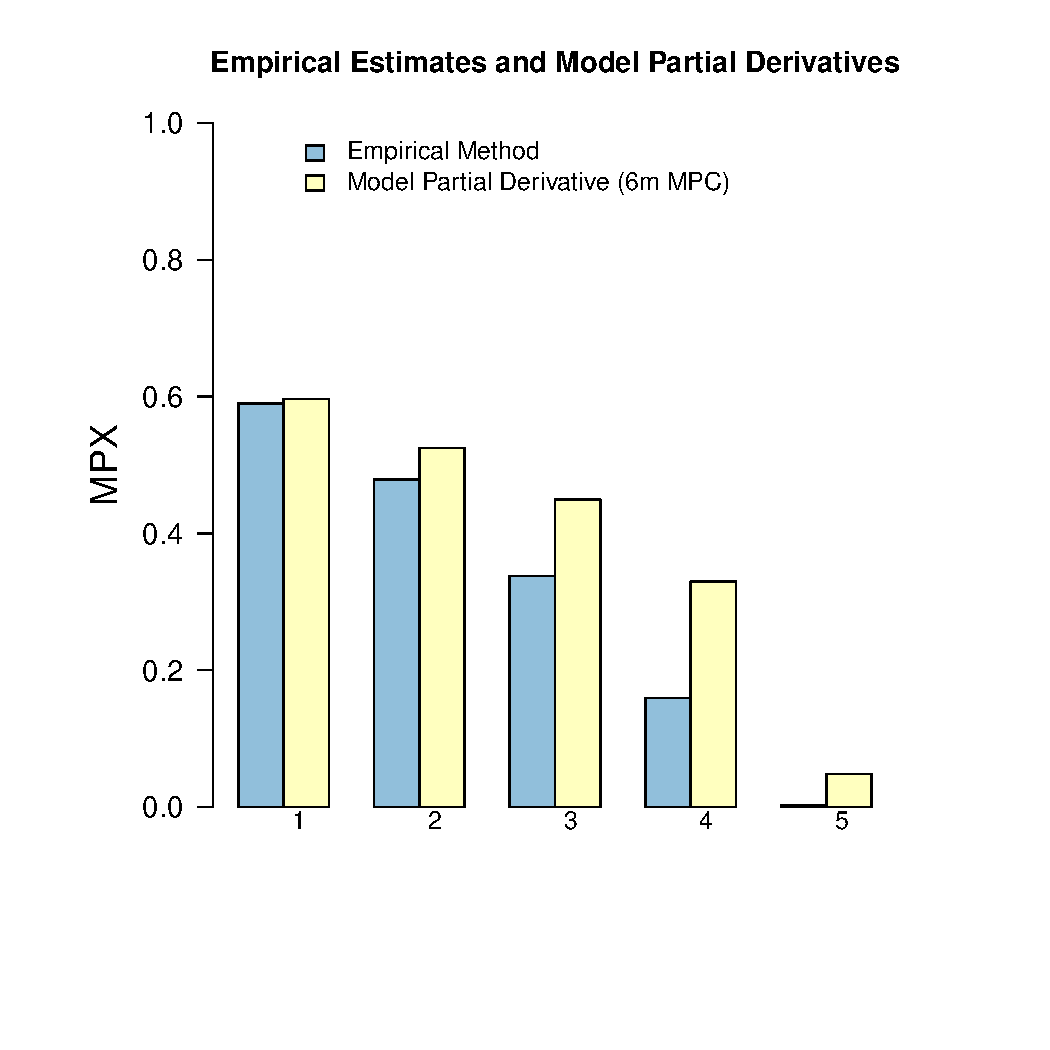
\includegraphics[scale=0.4]{\econtexRoot/Figures/MPC_accuracy.pdf}
		\caption{Empirical Method on Simulated Data versus Partial Derivative}
		\label{fig:MPC_accuracy}
	\end{centering}
\end{figure}

Figure \ref{fig:MPC_accuracy} shows how the empirical method performs on data simulated from the preference shock model of section \ref{model}. The method works well when the MPX is high, but overestimates the MPX when it is low, which is a direct result of the assumption that the consumption response to a transitory shocks decays within a two year period. The consumption response in the model is very close to the exponential decay model previously simulated, so it is not surprising that the bias is large for low values of the MPX. As above, empirical evidence suggests that, even for households with low MPX, the initial decay of the consumption response occurs much faster than exponential decay would suggest.

\section{Labor Elasticity} \label{labor_elasticity}
The empirical results of this paper estimate MPX to be at the high end of the literature. The results also conflict with standard consumption theory, particularly at the higher end of the liquid wealth distribution. It is possible that these high transitory MPX estimates are being driven by reverse causality: in years when households wish to spend more, they increase their labor supply. In this case, our assumption that labor income is exogenous would be false. To get a sense of the quantitative magnitude of the bias such reverse causality could induce, in online appendix \ref{labor_elasticity_model} we calibrate a model with both preference shocks and labor supply elasticity. We find the effect is quantitatively small, with both the true MPX and the estimates using our method being close to zero for a simulation of households with liquid wealth in the top quintile. However, for extreme values of preference shocks and labor elasticity, we can generate estimates of the transitory MPX to be as high as 0.25, when the true MPX is 0.08.\footnote{Estimates of the Frisch elasticity in microdata studies range from 0 to 0.5, while macroeconomic studies generally find a much larger elasticity of between 2 and 4 (see \cite{peterman_reconciling_2016}). We do not consider estimates of the Frisch elasticity in the macroeconomic range, as it seems likely to us that these estimates are high due to labor market frictions over the business cycle, rather than genuine labor supply choices of households. Some of the best evidence comes from \cite{cesarini_effect_2017}, who use lottery winnings in Sweden to estimate a Frisch elasticity of 0.14. The extreme values referred to in the text are a Frisch elasticity of 0.5 and an annual preference shock standard deviation of 0.4.}

\subsection{Labor Elasticity Model} \label{labor_elasticity_model}
\setcounter{figure}{0}   
\setcounter{table}{0} 
Here we detail the model and simulation results summarized in section \ref{labor_elasticity}. The model extends the standard incomplete markets model from section \ref{model}, incorporating both preference shocks, so that households have some years when their utility of consumption is greater than others, and labor elasticity, so that households can adjust their income based on the marginal utility of consumption. The household's problem is to maximize expected lifetime utility:
\begin{align*}
\mathbb{E}_t \sum_{n=t}^{\infty} \beta^n \Bigg(\mathcal{X}_n \frac{ \cLevBF_n^{1-\rho}}{1-\rho}-\frac{\lLevBF_n^{1+\frac{1}{\xi}}}{1+\frac{1}{\xi}} \Bigg)
\end{align*}
subject to the constraints:
\begin{align*}
\aLevBF_t = \mLevBF_t - \cLevBF_t \\
\bLevBF_t = R\aLevBF_t \\
\yLevBF_t =  l_t w_t \\
\lLevBF_t = l_t \pLevBF_t^{\frac{1-\rho}{1+\frac{1}{\xi}}}\\
w_t = \theta_t \pLevBF_t \\
\pLevBF_t = \Psi_t \pLevBF_{t-1} \\
\mLevBF_t = \bLevBF_t + \yLevBF_t
\end{align*}
The normalization of labor $(\lLevBF_t = l_t (\pLevBF_t^{\frac{1-\rho}{1+\frac{1}{\xi}}}))$ is set up to allow labor supply to move elastically with transitory income, but the long-run supply of labor does not depend on permanent income (as observed in the consistency of hours worked over long time periods and across countries). The key additional features of this model are (i) the preference shock factor and (ii) the elasticity of labor.

Labor elasticity is controlled by the Frisch elasticity $\xi$. When the wage (relative to permanent income) increases by $x\%$, hours worked increase by $\xi\%$. We will examine values of the Frisch elasticity between 0 and 0.5 to cover the range of estimates from microeconomic studies.

\begin{center}
	\input\econtexRoot/Tables/beta_laborsupply50.tex	
	\input\econtexRoot/Tables/TranShk_laborsupply50.tex		\captionof{table}{Fitted Discount Factors and Transitory Shock Standard Deviation}
	\label{table:fitted_beta_and_transtd}
\end{center}

\begin{center}
	\input\econtexRoot/Tables/phi_laborsupply50.tex	
	\input\econtexRoot/Tables/c_std_laborsupply50.tex		\captionof{table}{Simulation Estimates of $\phi$ and Consumption Growth Standard Deviation}
	\label{table:phi_laborsupply}
\end{center}

\begin{center}
	\input\econtexRoot/Tables/mpc_laborsupply50.tex
	\input\econtexRoot/Tables/psi_laborsupply50.tex		\captionof{table}{Simulation Estimates of MPC and $\psi$}
	\label{table:psi_mpc_laborsupply}
\end{center}

In tables \ref{table:fitted_beta_and_transtd}, \ref{table:phi_laborsupply}, and \ref{table:psi_mpc_laborsupply}, we have varied the size of the Frisch elasticity and annualized preference shock. In each cell we have kept constant the overall annualized income growth variance and the median liquid asset to annual income ratio.\footnote{We calibrate to an annualized growth variance of 0.01 and a median liquid asset to annual income ratio of 0.5 to approximately match the upper quintile of the liquid wealth distribution.} To achieve this we vary the discount factor and the variance of transitory wage shocks.

Table \ref{table:fitted_beta_and_transtd} shows how the discount factor, $\beta$, and the annualized transitory shock standard deviation vary. As the size of the preference shocks increase, so does the precautionary motive for households. As we have fixed the median amount of precautionary savings, the discount factor drops slightly to compensate. The right-hand panel shows that the standard deviation of transitory shocks required to match the overall level of income growth variance goes down as labor supply elasticity increases, which is as expected---when the transitory wage is low, households will work fewer hours. This amplifies the variance of the transitory income shock relative to the wage shock. The size of the preference shocks has little effect on the imputed size of the transitory shocks.

The left-hand panel of table \ref{table:phi_laborsupply} shows the estimate of $\phi$ (the MPX out of permanent shocks) is close to 1 for variations of preference shocks and labor elasticities. This is unsurprising, as labor does not respond to a change in permanent income. The right-hand panel shows a very significant increase in the standard deviation of consumption growth as the size of the preference shocks increases. With no preference shocks, the standard deviation of consumption growth (0.05) is about half of the standard deviation of income (0.1). As the size of preference shocks increases, so does consumption growth variance, with the standard deviation growing to 0.26 for large preference shocks. This standard deviation is still much smaller than 0.37, which comes directly from the data; however, the high number from the data is likely to be contaminated with measurement error in assets. A further consideration is that much of the observed variance in expenditure growth will be due to durable items, such as home improvements and vehicles. We analyzed the effect of durables on our estimates in section \ref{durables}, but, to the extent that these goods can be financed, our model with no borrowing may overestimate both the expenditure variance and the labor supply response to preference shocks.

Table \ref{table:psi_mpc_laborsupply} compares the actual mean MPC in the model with our empirical method for estimating the transitory expenditure elasticity. The left-hand panel shows that both preference shocks and labor elasticity, often both missing in consumption models for simplicity, have quantitatively significant impacts on the implied MPC. Increasing the Frisch elasticity from 0 to 0.5 (the full range of micro-estimates) decreases the six-month MPC from 6\% to just 3\%, because households now have an extra tool with which to insure against low consumption. When they receive a negative transitory shock to their wealth, they will consume less, which in turn will increase their marginal utility of consumption and induce them to work more hours. Therefore their actual income loss will be lower than the shock to their wealth and they will reduce their consumption by less than if they were unable to adjust their labor supply. In contrast, increasing the size of the preference shocks greatly increases the MPC as a result of the higher precautionary savings motive and consequently lower discount factor, even while median savings are unchanged.

The right-hand panel of table \ref{table:psi_mpc_laborsupply} shows the effect of preference shocks and labor elasticity on our empirical estimates of $\psi$, the transitory MPX. The top row shows that our estimate is lower than the MPC (due to the fact that at these low levels of MPC, more than two years is required for the transitory effect to decay away). It does, however, follow the same pattern as the MPC and falls in magnitude as the ability of households to adjust labor supply increases. Similarly, going down the first row shows that the estimated MPX increases with the preference shock. However, the similarity to the MPX table ends when we increase \textit{both} labor elasticity \textit{and} the size of the preference shocks. Our estimate can grow large, up to a value of 0.25, when extreme values are chosen: a Frisch elasticity of 0.5 and a preference shock standard deviation of 0.4. This measured transitory MPX now bears little relation to the MPX (which is 0.08). Instead, it is being driven by reverse causality, whereby preference shocks are driving consumption along with the decision to increase labor. The observed ``shocks'' to income are therefore highly correlated with consumption, but they are not causing the consumption dynamics exogenously.

This exercise suggests the bias due to reverse causality is likely to be small, but further investigation may be worthwhile.
\end{comment}

\section{Durables}\label{durables_appendix}
In this appendix we expand on section \ref{durables} on durable expenditure. First, it will help to write down a simple model. The model will show that our empirical methodology continues to estimate the consumption response to permanent and transitory shocks, but that these need to be interpreted carefully. The model uses the same income process as section \ref{cov_restrictions}. Remembering the income process is made up of two martingale processes, $P_t$ and $Q_t$, which may have jumps, instantaneous income is given by
\begin{align*}
dy_t = \Big( \int_{0}^{t}dP_s \Big) dt  +dQ_t 
\end{align*}
while instantaneous expenditure now has both a durable and a nondurable component:
\begin{align*}
dc_t = \phi_{nd} \Big( \int_{0}^{t} dP_s  \Big) dt + \phi_{d} dP_t + \psi dQ_s
\end{align*}
Here we have assumed that the expenditure response to transitory shocks is instantaneous, but it would not change things to assume as before that the response decays to zero after two years. However, it is important that the durable component of the expenditure response to permanent shocks occurs instantaneously with the shock (or very soon after). Aggregating income and consumption annually gives
\begin{align*}
\Delta^N \bar{y}_T &=  \Big(\int_{T-N-1}^{T-N} (s-(T-N-1))dP_s  + \int_{T-N}^{T-1}dP_s + \int_{T-1}^{T} (T-s)dP_s \Big) \\
& \qquad + \Big(\int_{T-1}^{T} dQ_t -\int_{T-N-1}^{T-N} dQ_t \Big) \\
\Delta^N \bar{c}_T &= \phi_{nd} \Big(\int_{T-N-1}^{T-N} (s-(T-N-1))dP_s  + \int_{T-N}^{T-1}dP_s + \int_{T-1}^{T} (T-s)dP_s \Big) \\
& \qquad + \phi_d \Big(\int_{T-1}^{T} dP_t -\int_{T-N-1}^{T-N} dP_t \Big) \\
& \qquad + \psi \Big(\int_{T-1}^{T} dQ_t -\int_{T-N-1}^{T-N} dQ_t \Big) \\
\end{align*}
From this we can calculate the covariance:
\begin{align*}
\mathrm{Cov}(\Delta^n \bar{c_T},\Delta^n \bar{y_T} ) &= \phi_{nd} \mathrm{Var}(\Delta^n \bar{y_T}) \\
& \qquad + \phi_d \Bigg( \int_{T-1}^{T} (T-s) \sigma_P^2 dt - \int_{T-N-1}^{T-N}(s-(T-N-1)) \sigma_P^2 dt \Bigg) \\
& \qquad + \psi\Bigg(\int_{T-1}^{T}  \sigma_Q^2 dt + \int_{T-N-1}^{T-N}\sigma_Q^2 dt\Bigg) \\
&= \phi_{nd} (n-\frac{1}{3})\sigma_P^2 + 0 +  2 \psi \sigma_Q^2
\end{align*}
So the durable component of the covariance cancels out, and our identification method correctly identifies $\phi_{nd}$ and $\psi$ but is unable to identify $\phi_d$.

However, if there is some delay between the household receiving the permanent income shock and purchasing the durable goods, then this introduces an upward bias into the estimate of transitory MPX. The size of the bias grows with the number of months delay between the permanent income shock and the durable goods purchase, plateauing after 12 months at a level of $\frac{\sigma^2_p}{2\sigma^2_q}\phi_d$. Figure \ref{fig:durable_bias} shows how this bias increases with the delay.
\begin{figure} 
	\begin{centering}
		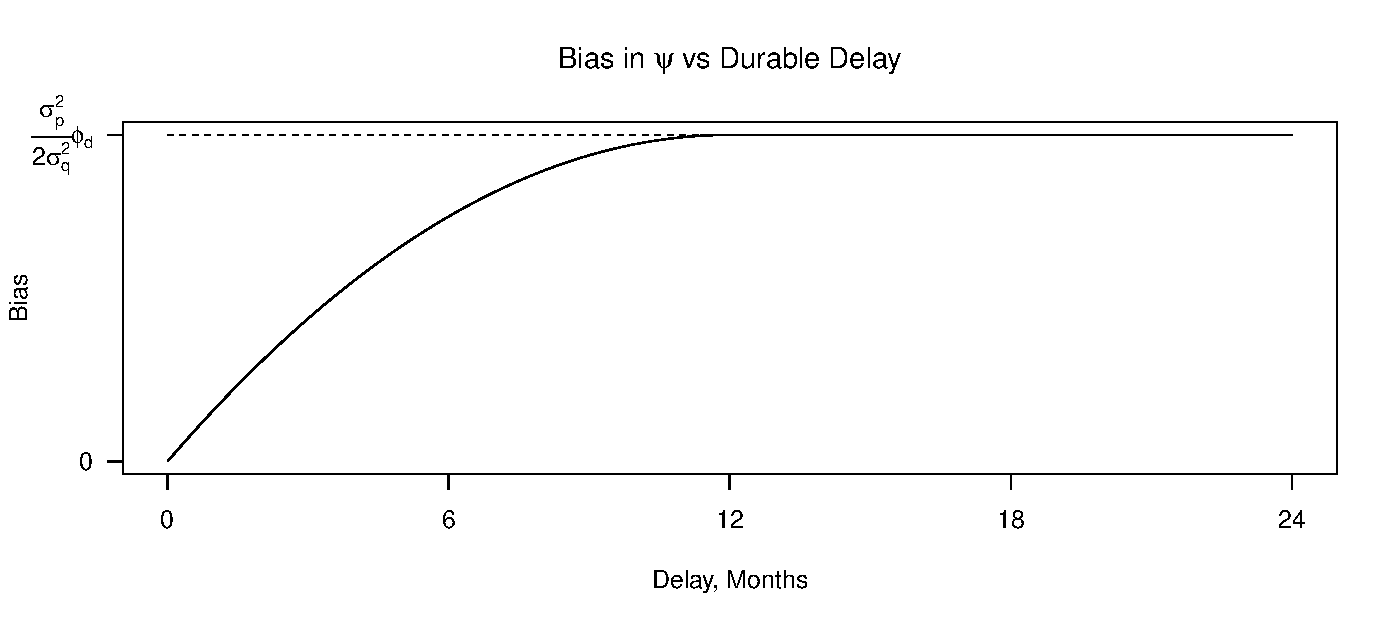
\includegraphics[scale=0.6]{\econtexRoot/Figures/DurableBias.pdf}
		\caption{Bias in Transitory MPX with Delay in Durable Goods Purchase}
		\label{fig:durable_bias}
	\end{centering}
\end{figure}

In order to quantify how large this bias may be in practice, we make use of the car registry data available in Denmark. Using data on the current value of cars owned by a household, we perform the same residual calculation to find the change in car value that is unpredictable with the household characteristics we are able to observe. We then construct two new expenditure panels: one in which we remove expenditures on cars, and one in which we make a proxy for non-durable consumption by removing expenditures on cars multiplied by $\frac{1}{0.421}$ (car purchases make up 42.1\% of durable expenditure in Denmark):
\begin{align*}
C_T^{\text{nocar}} = C_T - \Delta \text{CarValue} \\
C_T^{\text{nondurable}} = C_T - \frac{1}{0.421}\Delta \text{CarValue}
\end{align*}
The second, nondurable proxy consumption panel, can be modeled as the true non-durable consumption panel with classical measurement error added. This classical measurement error does not bias our estimates, so we can use this nondurable proxy panel to estimate an unbiased MPC out of transitory shocks, where the MPC does not include durable expenditures.

The results of this exercise can be seen in figure \ref{fig:MPXByDurables}. Even without bias, we would expect the nondurable proxy estimates to be lower than those including all expenditures, as the definition of transitory MPX changes over the three panels to exclude cars and then all durable goods. For the lower quintiles of liquid wealth it therefore looks as though the bias is likely very small, as nondurable goods make up 10\% of spending and the MPX estimates are smaller by approximately 10\% in this region. For the top quintile of liquid wealth there seems to be some bias, with the estimate of MPX for all expenditures decreasing from 25\% to an MPC for nondurable goods of 17\%.

While there is some evidence that our results may be biased upward for those in the top quintiles of liquid assets, this bias will only have a small effect on our overall conclusions. As the relevant number for the monetary policy exercise is the MPX rather than the MPC, we have chosen not to adjust our baseline results using this method and accept that a small bias may exist in our data. It should be noted that such a bias will cause the heterogeneous channels of monetary policy to appear smaller than they actually are.


\section{RIP or HIP Income Process?} \label{rip_hip_appendix}
\setcounter{figure}{0}   
\setcounter{table}{0} 
\subsection{RIP or HIP Income Process?} \label{rip_hip}
Our method makes strong assumptions on the income process---namely, that there is no persistent idiosyncratic component to income growth and that the process contains a random walk. \cite{guvenen_empirical_2009} shows that it is empirically difficult to distinguish between a `Restricted Income Profile' (RIP) like this and a `Heterogenous Income Profile' (HIP) income process, in which (i) shocks to income are much less persistent (e.g., AR(1) with $\rho\approx 0.8$), and (ii) households have a persistent idiosyncratic growth component. The reason the RIP and HIP processes are difficult to tell apart is that the two features (i) and (ii) act in opposite directions on the cross-section variance of income growth. The less persistent income shocks lead the cross-sectional income growth variance to not grow as fast as the HIP model, while the persistent idiosyncratic growth component leads the same variance to grow at a faster rate. The result is that the increase in variance of income growth over three to four years is approximately the same as the increase from four to five years. To the extent that the consumption response to these semi-permanent shocks is similar to the response to the idiosyncratic persistent growth component,\footnote{See \cite{guvenen_learning_2007} for an example of why this might be the case: if households do not know their own idiosyncratic growth ex-ante, a Bayesian learning process will be very slow, so households (at least initially) will react in similar ways to changes in income due to this persistent growth component as a true income shock.} our methodology will continue to provide reasonable estimates of the ``permanent'' MPX and the more familiar transitory MPX. 

Both the Restricted Income Profile (RIP) and Heterogeneous Income Profile (HIP) processes can be described by the equations:
\begin{align*}
	y_h^i = \beta^i h + z^i_h + \varepsilon^h_i\\
	z^i_h = \rho z^i_{h-1]} + \eta^h_i
\end{align*}
where $i$ indexes the worker and $h$ the years of experience. $\varepsilon^h_i$ represents a transitory shock to income, while $\eta^h_i$ is persistent. $\beta^i$ represents an idiosyncratic persistent growth factor.

In the RIP model, $\beta^i=0$ and $\rho$ is usually estimated to be very close to 1 (in this paper we assumed $\rho=1$). In the HIP model, $\beta^i$ has a cross-sectional variance $\sigma_{\beta}^2>0$, and $\rho$ is normally estimated to be significantly lower than 1, around 0.8. The reason these are difficult to tell apart is because the theory does not give a strong indication in which model the cross-sectional variance of income growth over $N$ years should grow faster. In the RIP model with $\rho=1$, the cross-sectional variance of income growth increases linearly with $N$. In the RIP model with $\rho\approx 0.8$, the growth in the  cross-sectional variance of income growth will decrease due to the low $\rho$ but increase due to the idiosyncratic $\beta^i$.

Figure \ref{fig:increasing_diff} shows the empirical values for income growth variance and the covariance of income and expenditure growth over $N$ years. We have also plotted the fitted values for these statistics that are implied by our model when fitted to $N=3,4,5$ as we do in the paper. We see the empirical variance and covariance decline slightly below the model fitted line as $N$ becomes large, which fits with the finding that $\rho$ in the RIP model is usually slightly below 1.0, around 0.98 or 0.99. We also note that around the region where we achieve our identification ($N=3,4,5$), there is very little curvature in the empirical statistics, and the increase in both variance and covariance is close to linear.

While this linearity around $N=3,4,5$ cannot help us distinguish between the RIP and HIP process, it does imply that our empirical methodology may be somewhat robust to misspecification along this dimension. If we assume that the expenditure response to a change in $z^i_h$ and to the increase from the persistent idiosyncratic growth are equal to $\phi$, and the response to a transitory shock is $\psi$, that is:
\begin{align*}
	\Delta^N c^i_h \approx \phi \Delta^N (\beta^i h + z^i_h) + \psi \Delta^N \varepsilon^h_i
\end{align*}
Then, the fact that $\mathrm{Var}\big( \Delta^N (\beta^i h + z^i_h) \big)$ grows approximately linearly with $N$ means that our empirical method will correctly identify $\phi$ and $\psi$.

A full investigation of the implications of different income processes is beyond the scope of this paper but would be a very useful exercise for future research.
	
\begin{figure} 
	\begin{centering}
		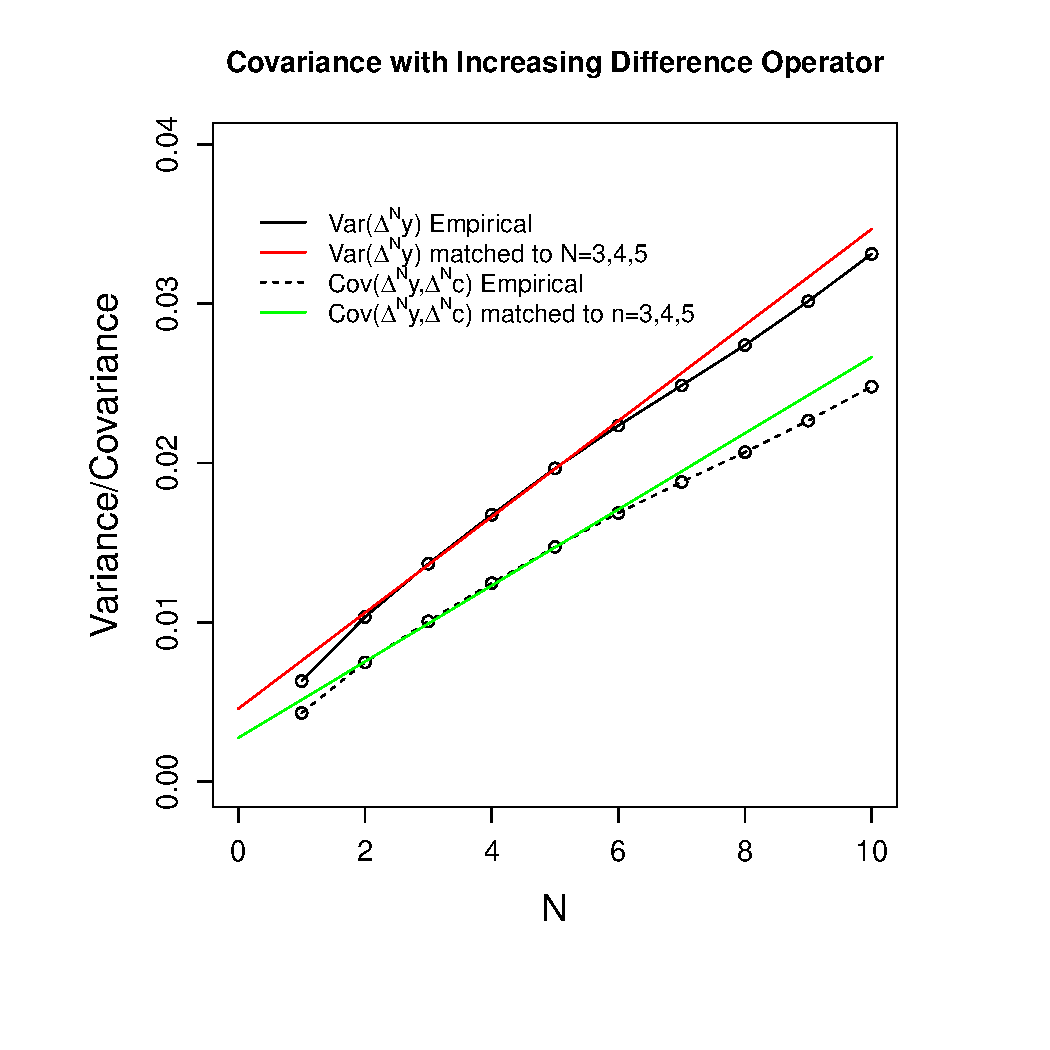
\includegraphics[scale=0.4]{\econtexRoot/Figures/IncreasingDiff_level_lincome_head.pdf}
		\caption{Variance and Covariance with Years of Growth}
		\label{fig:increasing_diff}
	\end{centering}
\end{figure}

\section{Time-Varying Risk} \label{time_varying_risk}
\setcounter{figure}{0}   
\setcounter{table}{0} 
We have assumed that idiosyncratic risk remains constant over time. Given that our sample period covers the great recession, this may not be appropriate. Here we show how the variance of income growth has varied over time, peaking just after the crisis in 2010. In order to test how much this time-varying risk might bias our results, we simulated data with $\phi=1$ and $\psi=0.5$, with permanent variance equal to estimates from the data and transitory variance varying in order to match the time-varying income risk pattern observed in the data. When we run this simulation we find estimates of $\phi$ and $\psi$ within 1\% of their true values.

Figure \ref{fig:income_growth_std} shows how the standard deviation of income growth has changed over the sample period. From trough to peak, the standard deviation increases approximately 10\%. In the simulation referred to in section \ref{time_varying_risk}, we assume that both transitory income and transitory consumption response have no persistence. We divide each year into 20 sub-periods, choose the variance of permanent shocks to be 0.003, and allow time-varying transitory shocks to match the pattern in figure \ref{fig:income_growth_std}. We choose values of $\phi=1$ and $\psi=0.5$ and apply our estimation procedure (that assumes constant variance) to the simulated data. We recover estimated values of $\phi$ and $\psi$ to be 1.006 and 0.499, respectively.
\begin{figure} 
	\begin{centering}
		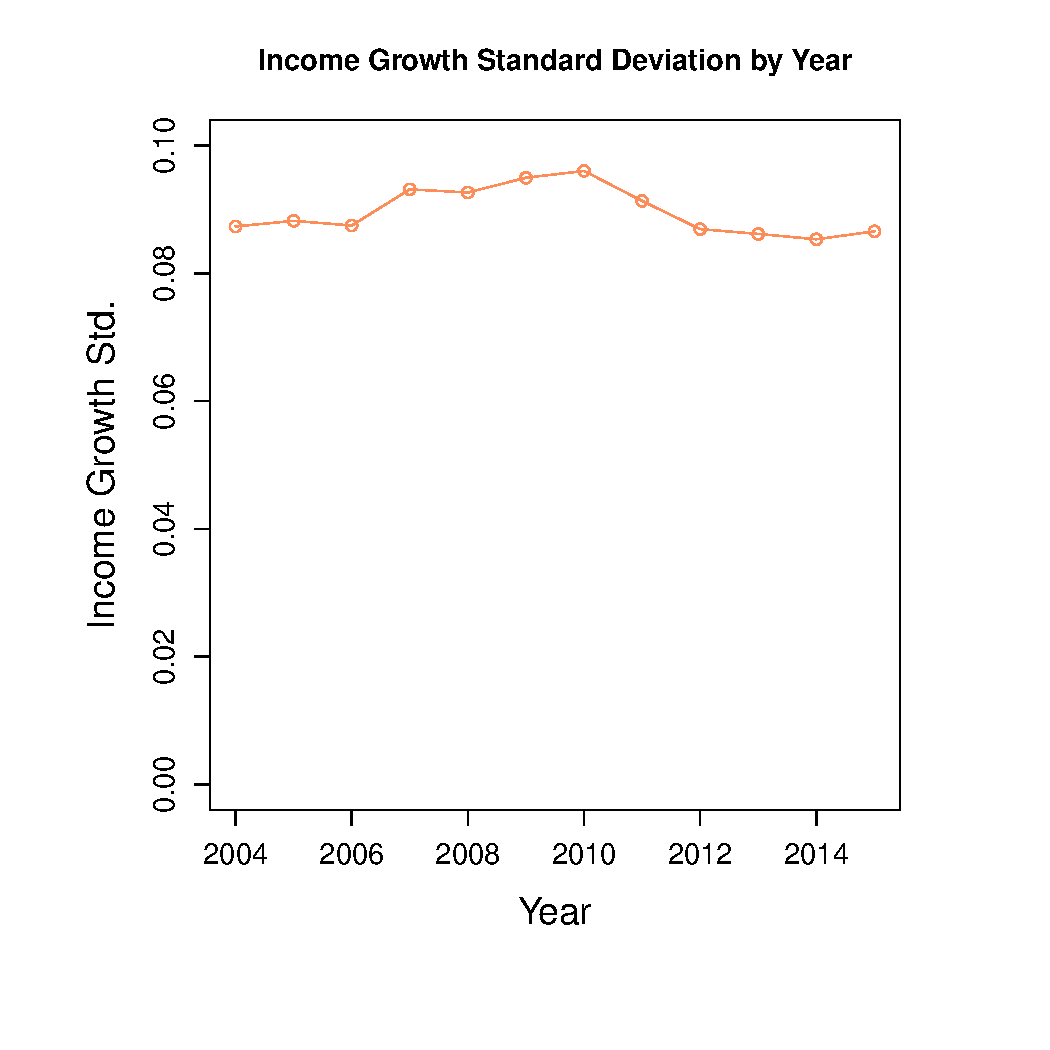
\includegraphics[scale=0.4]{\econtexRoot/Figures/IncomeGrowthStd.pdf}
		\caption{Standard Deviation of Income Growth}
		\label{fig:income_growth_std}
	\end{centering}
\end{figure}

\section{Robustness} \label{robustness}
As would be clear from the main text, we have made a number of choices regarding both data and variable definitions as well as more methodological issues. In a series of graphs, this appendix presents a number of robustness checks aimed at assessing the extent to which our results are sensitive to the specific choices. 

We begin with a number of robustness checks regarding our imputed expenditure measure, which may suffer from measurement error. In figure \ref{fig:Robust_liquidURE}, we compare our baseline estimates of the MPX to estimates based on different sample selection procedures. First, we exclude all households that own stocks corresponding to more than 10,000 USD (10\% of households in our sample). Second, we do not remove households that have negative imputed expenditure. We remove those households in our baseline sample because negative expenditure is clearly not a good estimate of actual expenditure. However, for example, in the event that negative expenditure arises because of classical measurement error, removal of negative estimates may be asymmetric and introduce an upward bias in average imputed expenditure. Third, to check that large outliers do not drive our results, we remove observations in the top and bottom 2.5\% in terms of level and change of income and expenditure. In the baseline calculations, we use only a 1\% cutoff. Our results are qualitatively unchanged when using these alternative approaches to take account of measurement error. In terms of magnitudes of the estimated MPXs, the largest difference to the baseline results seems to be found when we include negative expenditure estimates. As expected, this makes the largest difference among the wealthier households. The specification of outliers also matters somewhat for the point estimates of MPX in certain groups of households, but differences are not large. 

\begin{figure}
	\begin{centering}
		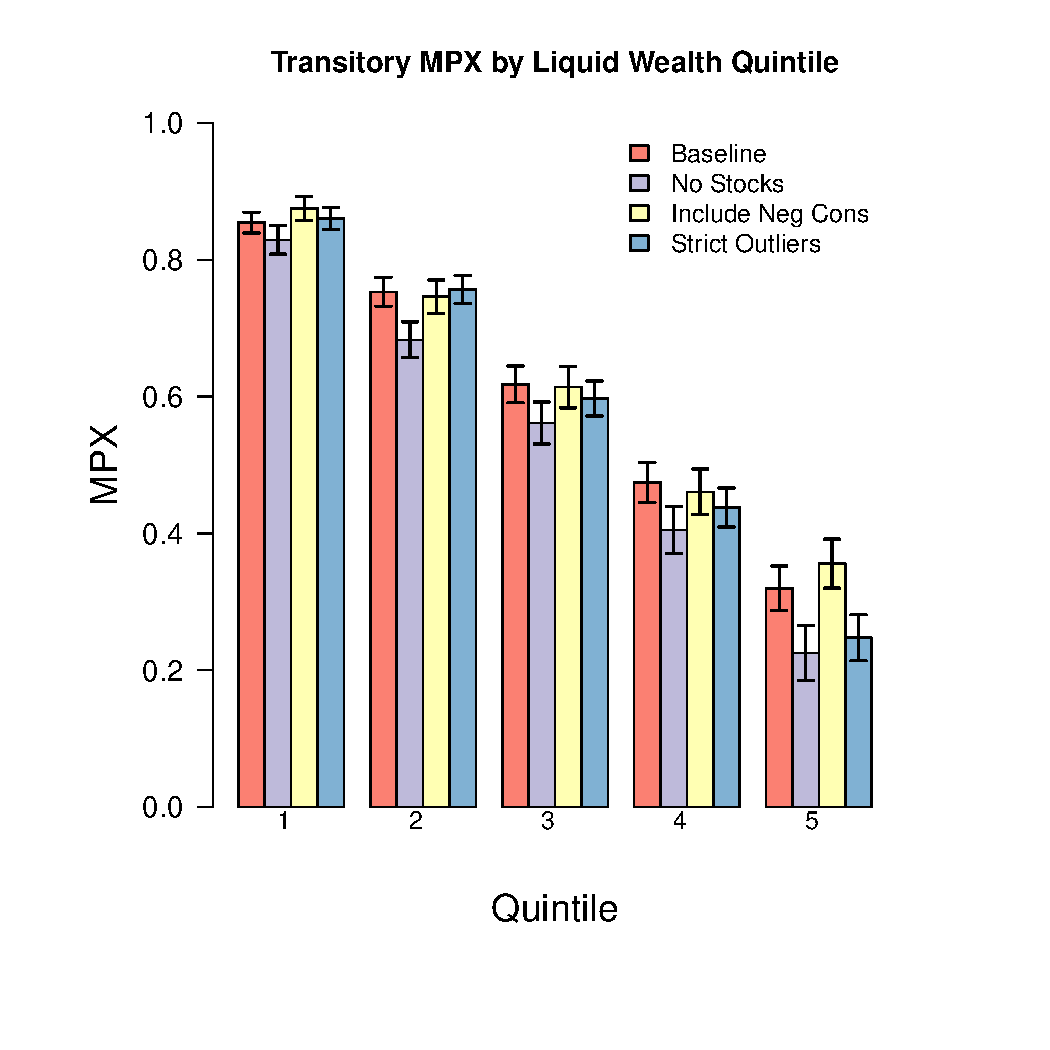
\includegraphics[scale=0.4]{\econtexRoot/Figures/Robust_tranMPX_liquidwealth.pdf}
		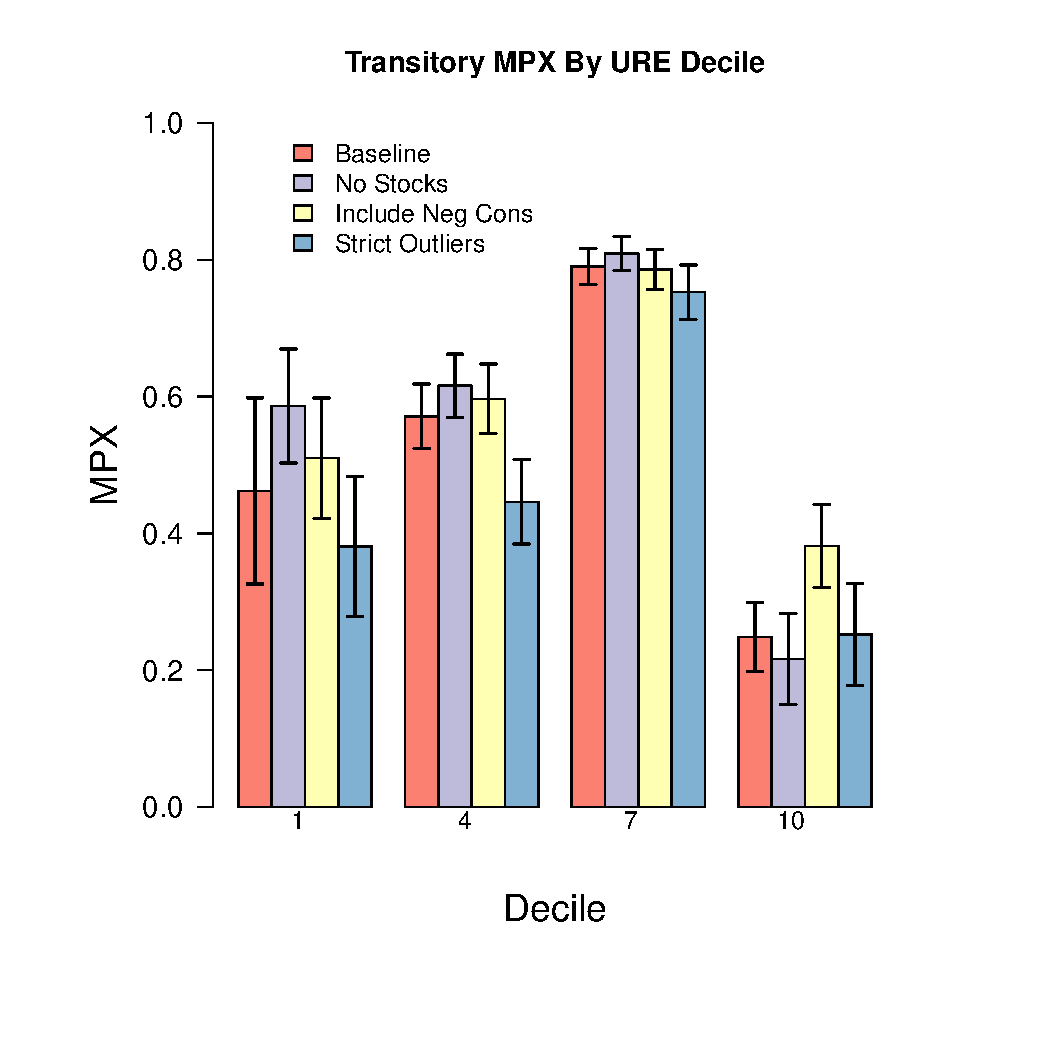
\includegraphics[scale=0.4]{\econtexRoot/Figures/Robust_tranMPX_URE.pdf}
		\caption{Robustness of Liquid Wealth and URE Distributions}
		\label{fig:Robust_liquidURE}
	\end{centering}
\end{figure}

Another robustness check consists of specifying consumption and income in logs rather than in levels. The fundamental difference is that the log specification yields an elasticity rather than an MPX. Hence, some difference between level and log results must be expected for households that only spend a fraction of their annual income (typically wealthier households). Indeed, as expected, figure \ref{fig:Robust_Logs} demonstrates that results hold qualitatively when specifying income and expenditure in logs rather than in levels, whereas estimated elasticities are higher than the MPXs for the wealthier households and those with high URE. Time-varying income risk may also potentially contribute to differences between results based on levels and logs. However, as shown in section \ref{time_varying_risk}, this is not likely to be important in our setting.  

\begin{figure} 
	\begin{centering}
		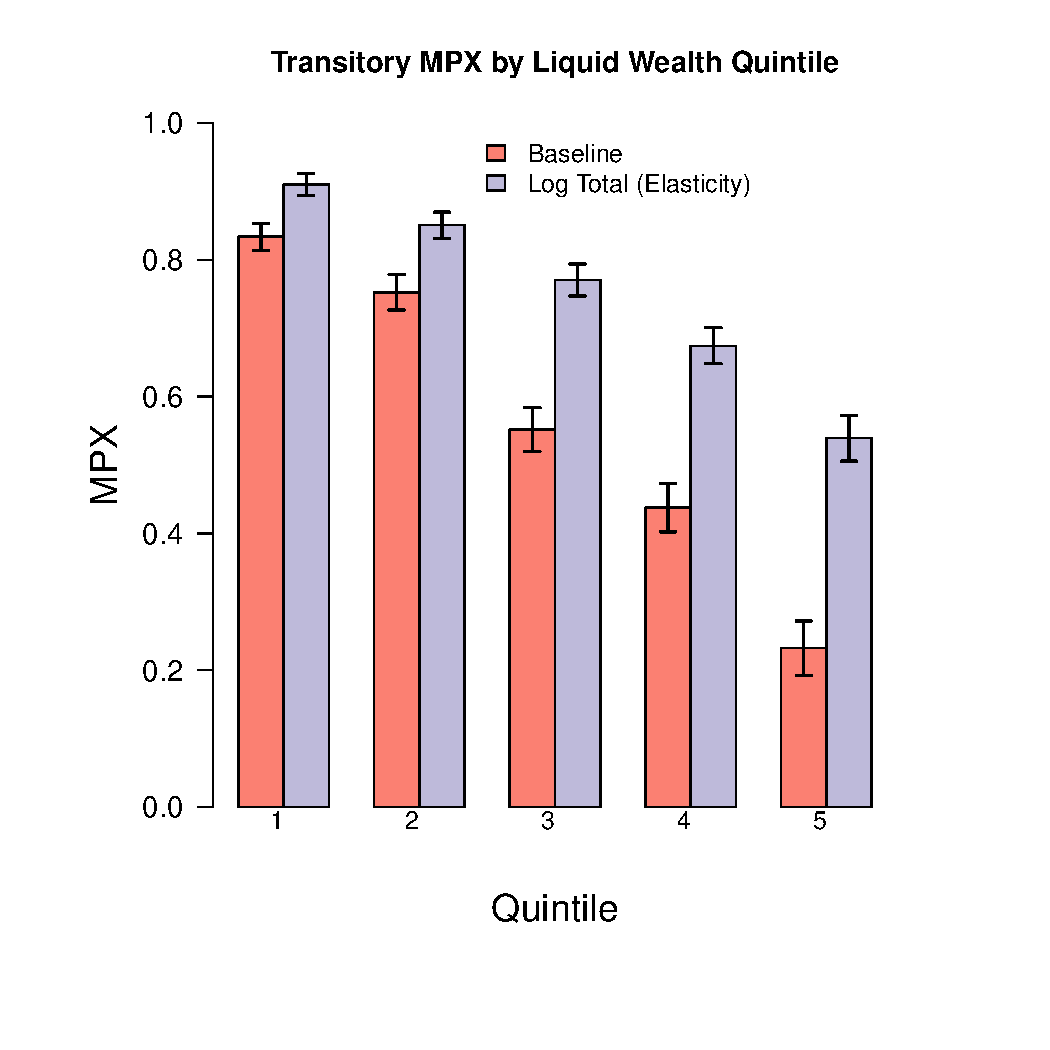
\includegraphics[scale=0.4]{\econtexRoot/Figures/Logs_tranMPX_liquidwealth.pdf}
		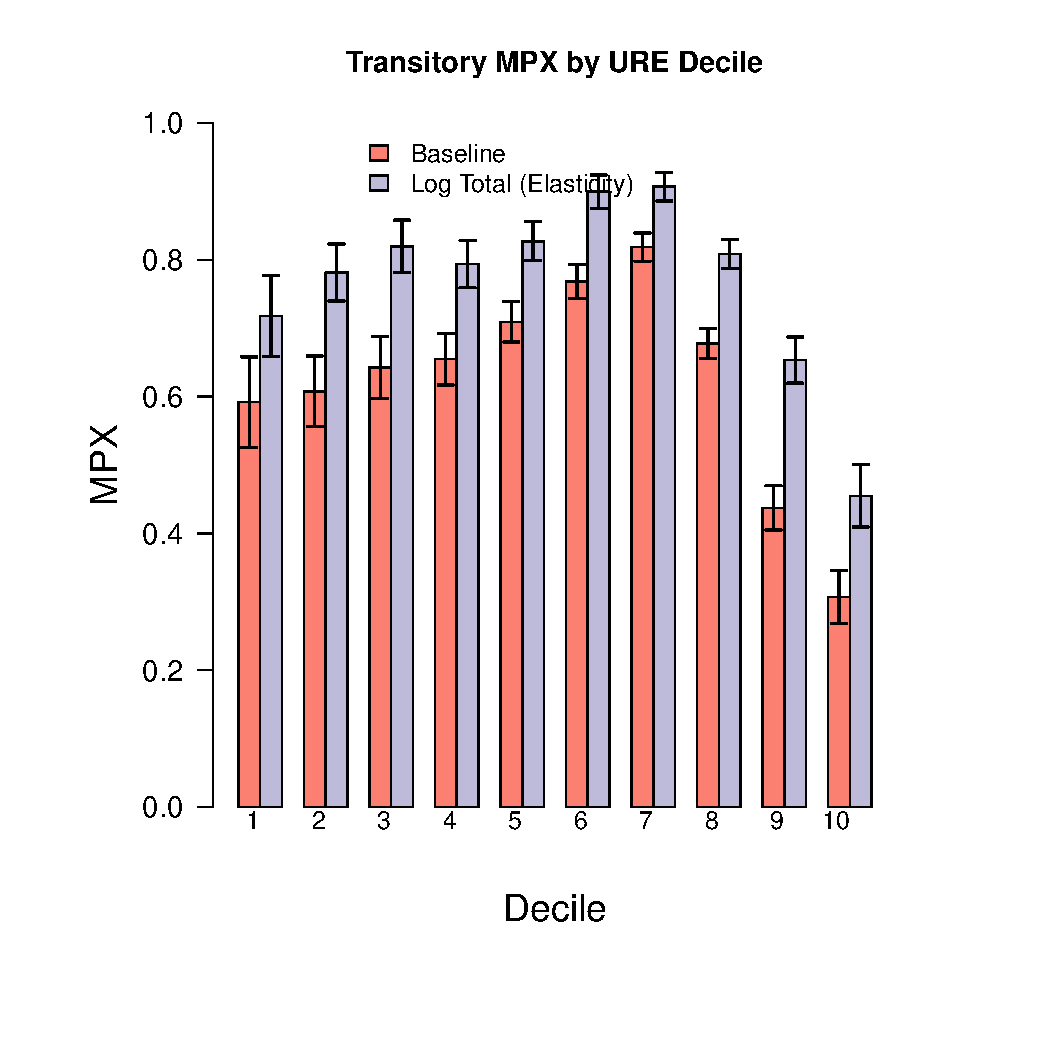
\includegraphics[scale=0.4]{\econtexRoot/Figures/Logs_tranMPX_URE.pdf}
		\caption{Results Using Log Income and Expenditure}
		\label{fig:Robust_Logs}
	\end{centering}
\end{figure}

As discussed in section \ref{income}, we use labor income of the head of the household as our prime measure of income in line with previous literature. Various mechanisms---e.g., intra-household income insurance---may give rise to differences between results based on income of the head of household and total household income. However, figure \ref{fig:Robust_TotalvsHead} demonstrates that there is virtually no difference in our results between using total household income and only the household head's income. Online appendix \ref{Insurance} briefly discusses the potential role that intra-household insurance may play, which we leave as an area for future research. 

\begin{figure} 
	\begin{centering}
		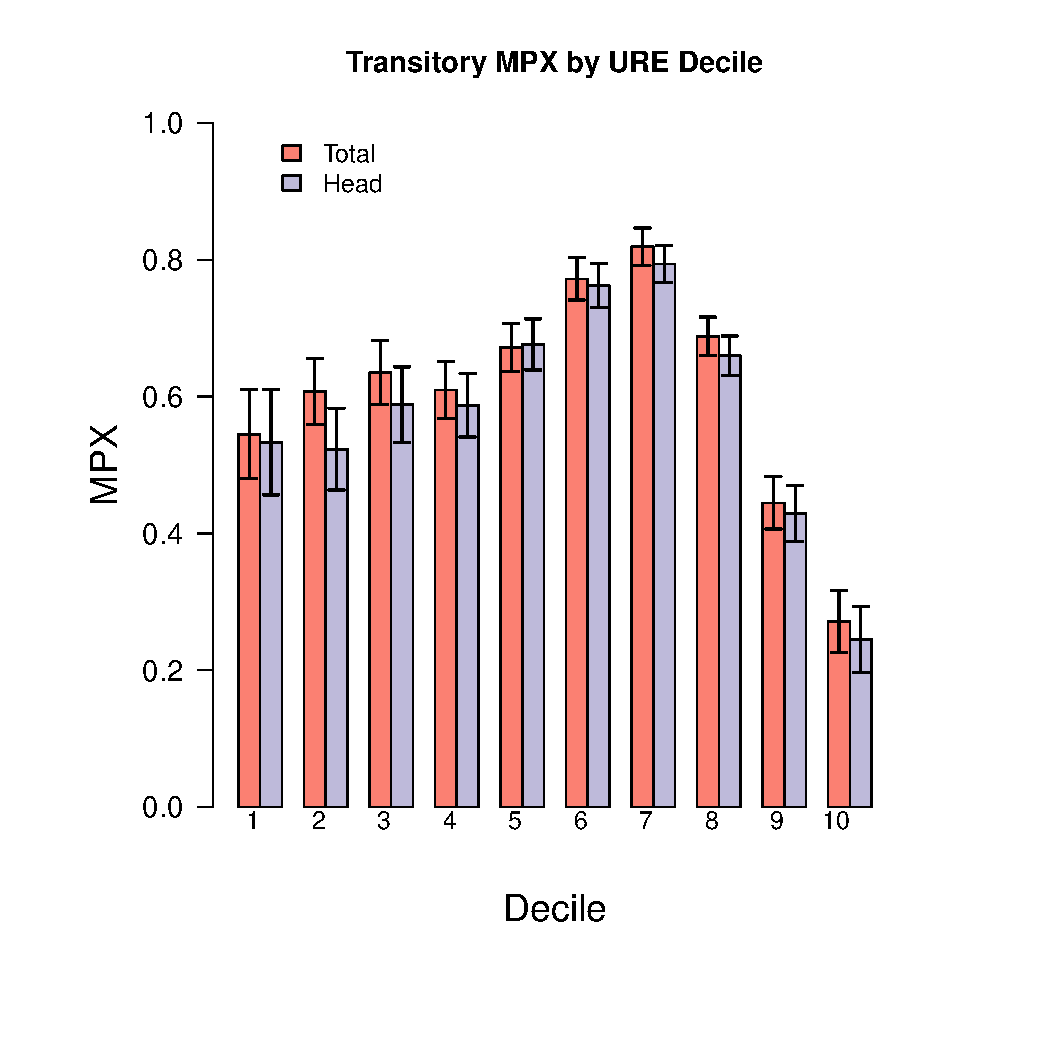
\includegraphics[scale=0.4]{\econtexRoot/Figures/total_tranMPX_URE.pdf}
		\caption{Results Using Total Labor Income and Head Labor Income}
		\label{fig:Robust_TotalvsHead}
	\end{centering}
\end{figure}

Finally, figure \ref{fig:MPXByLiquidWealth} shows the distribution of MPX by quintile of liquid wealth. It might be argued that the relevant level of liquid wealth is relative to income rather than in absolute terms. Figure \ref{fig:Robust_DivPerm} demonstrates that results based on quintiles of liquid wealth divided by permanent income are similar. Also, results (not shown here) where deciles are based on a broader definition of liquid wealth---i.e., including stock and bond holdings---are similar to our baseline results. 

\begin{figure} 
	\begin{centering}
		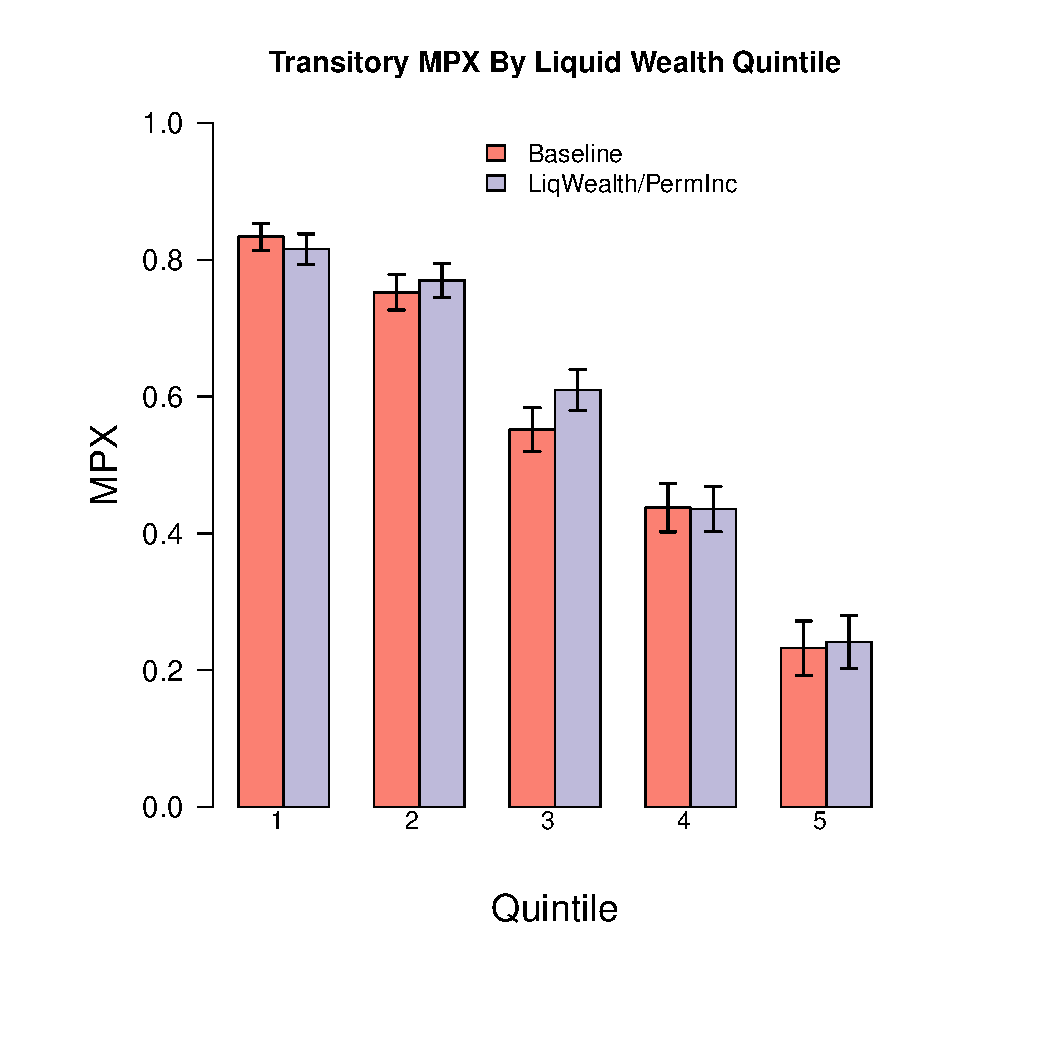
\includegraphics[scale=0.4]{\econtexRoot/Figures/DivPerm_tranMPX_liquidwealth.pdf}
		\caption{Results Using Quintiles of Liquid Wealth over Permanent Income vs Liquid Wealth}
		\label{fig:Robust_DivPerm}
	\end{centering}
\end{figure}


\section{Distribution of Permanent MPX by NNP, URE, and Income} \label{PermMPXbyURENNP}
\setcounter{figure}{0}   
\setcounter{table}{0} 
Figure \ref{fig:MPCAuclert_perm} shows the distribution of both transitory and permanent MPX by NNP, URE and income decile. The transitory numbers are a repeat of figure \ref{fig:MPCAuclert}.
\begin{figure} 
	\begin{centering}
		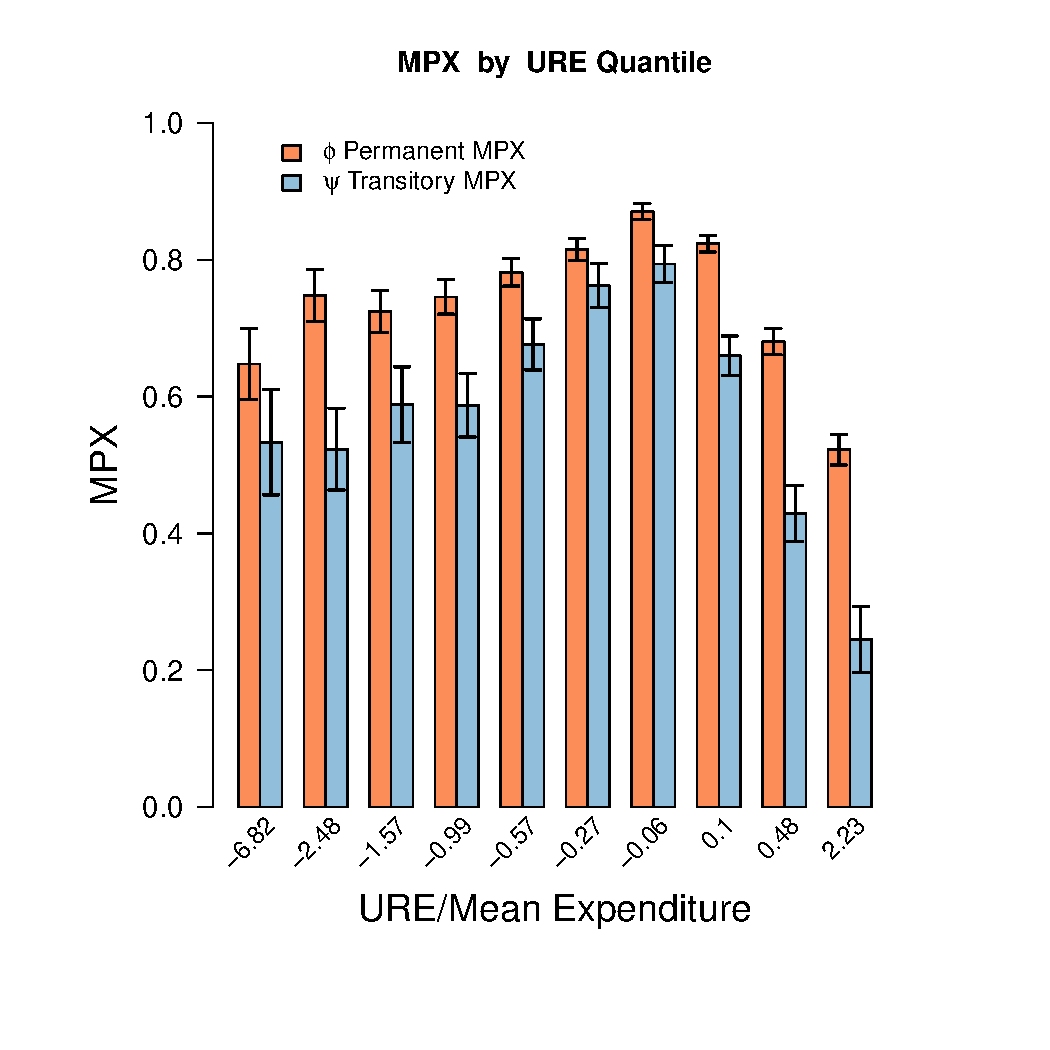
\includegraphics[scale=0.4]{\econtexRoot/Figures/MPXBypermURE_level_lincome_head.pdf}
		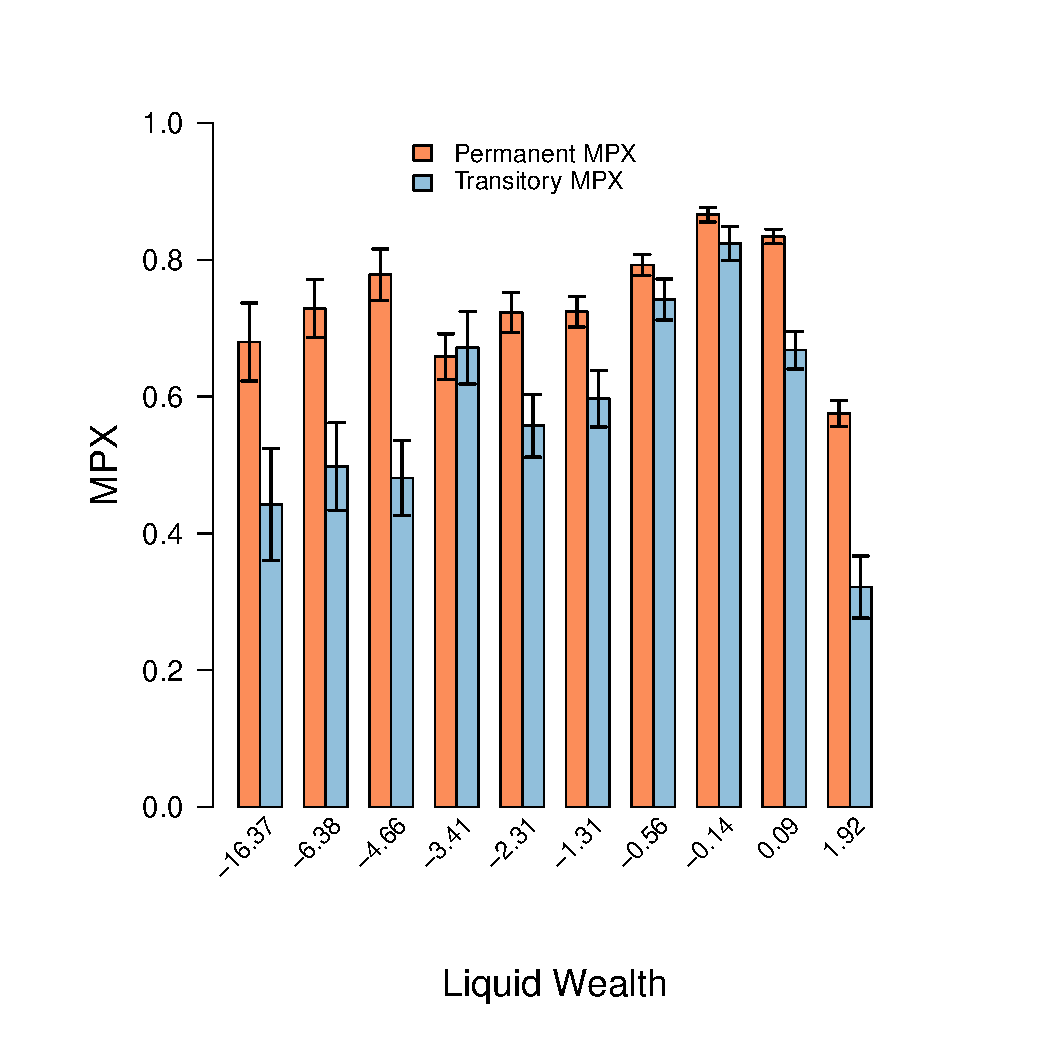
\includegraphics[scale=0.4]{\econtexRoot/Figures/MPXBypermNNP_level_lincome_head.pdf}
		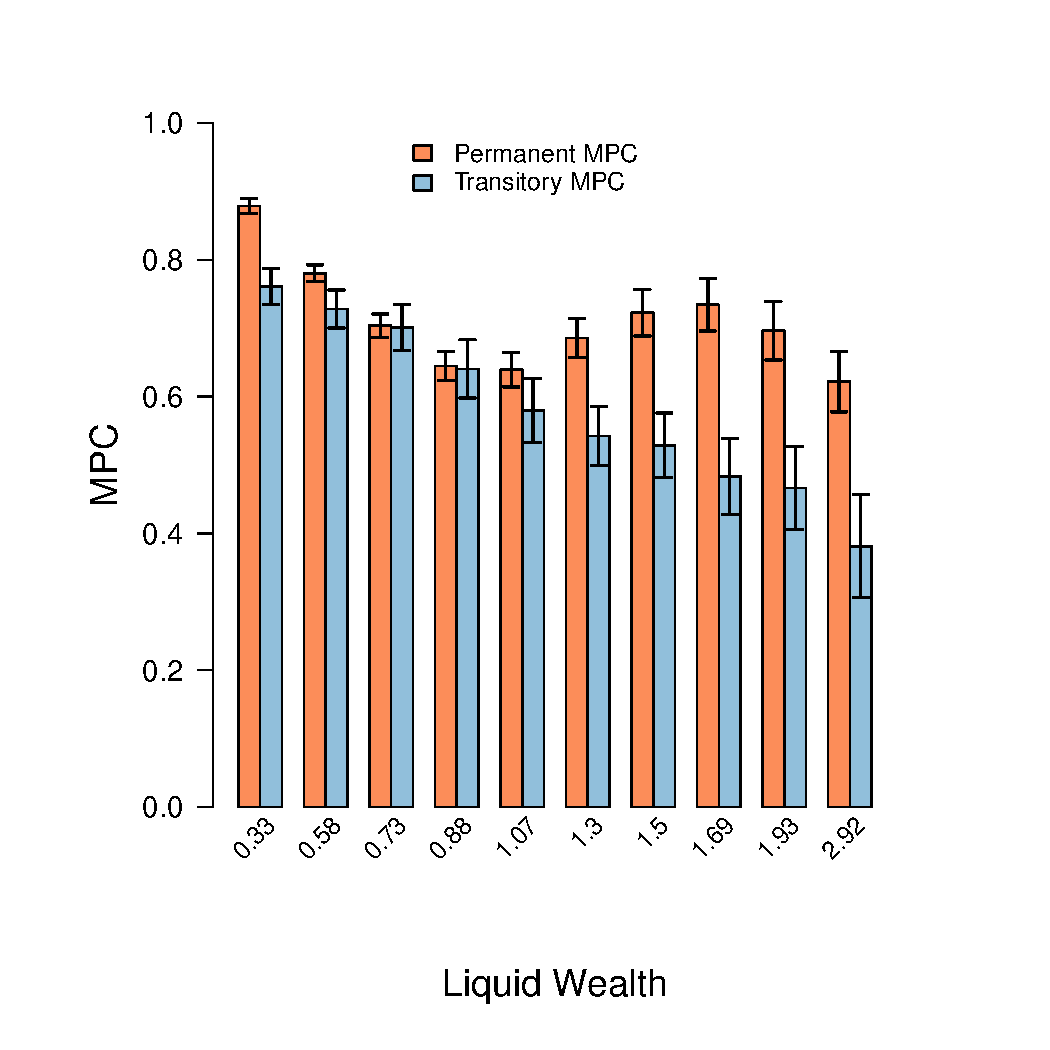
\includegraphics[scale=0.4]{\econtexRoot/Figures/MPXBypermIncome_level_lincome_head.pdf}
		\caption{MPX Distribution by URE, NNP, and Income}
		\label{fig:MPCAuclert_perm}
	\end{centering}
\end{figure}

\section{Intra-household Income Insurance} \label{Insurance}
\setcounter{figure}{0}   
\setcounter{table}{0} 
As discussed in section \ref{income}, we use labor income of the head of the household as our prime measure of income, in line with previous literature. Figure \ref{fig:Robust_TotalvsHead} demonstrates that results based on total household income and income of the head of household are similar. However, MPXs from transitory shocks to the income of the spouse are lower than MPXs from shocks to total income, in particular for the less wealthy households, as demonstrated in figure \ref{fig:Robust_Spouse}. This indicates heterogeneity in the role that intra-household income insurance plays across different groups of households. We leave this interesting topic for future research. 


\begin{figure} 
	\begin{centering}
		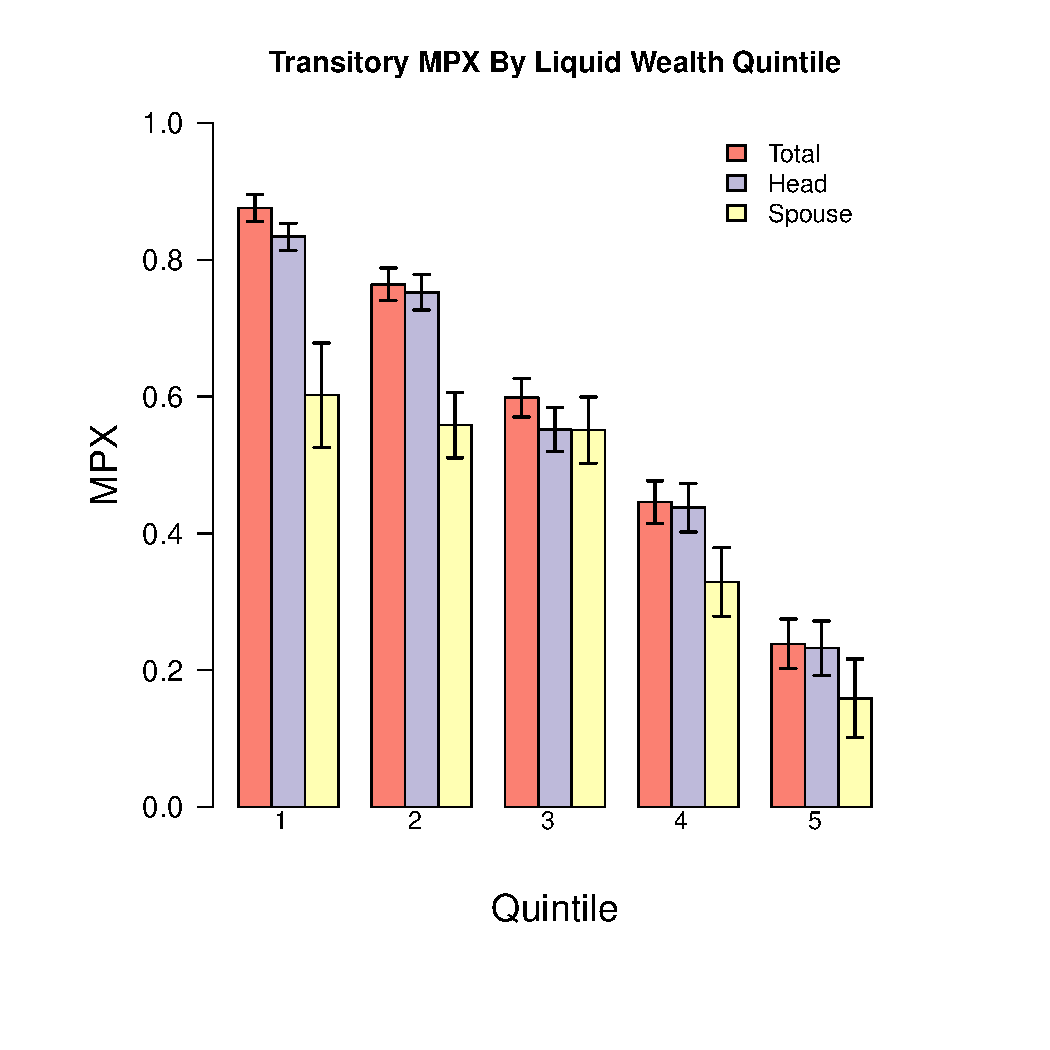
\includegraphics[scale=0.4]{\econtexRoot/Figures/Spouse_tranMPX_liquidwealth.pdf}
		\caption{Results Using Total, Head, and Spouse Labor Income}
		\label{fig:Robust_Spouse}
	\end{centering}
\end{figure}

%\section{Simulation Results}\label{sec:Simulation}
%\input\econtexRoot/Appendices/Simulation.tex


%\AtEndDocument{
\includepdf[pages=-]{Backpage.pdf}}

\end{document}









